\documentclass[]{book}
\usepackage{lmodern}
\usepackage{amssymb,amsmath}
\usepackage{ifxetex,ifluatex}
\usepackage{fixltx2e} % provides \textsubscript
\ifnum 0\ifxetex 1\fi\ifluatex 1\fi=0 % if pdftex
  \usepackage[T1]{fontenc}
  \usepackage[utf8]{inputenc}
\else % if luatex or xelatex
  \ifxetex
    \usepackage{mathspec}
  \else
    \usepackage{fontspec}
  \fi
  \defaultfontfeatures{Ligatures=TeX,Scale=MatchLowercase}
\fi
% use upquote if available, for straight quotes in verbatim environments
\IfFileExists{upquote.sty}{\usepackage{upquote}}{}
% use microtype if available
\IfFileExists{microtype.sty}{%
\usepackage{microtype}
\UseMicrotypeSet[protrusion]{basicmath} % disable protrusion for tt fonts
}{}
\usepackage[margin=1in]{geometry}
\usepackage{hyperref}
\hypersetup{unicode=true,
            pdftitle={Modern R in a Corporate Environment},
            pdfauthor={Brian Davis},
            pdfborder={0 0 0},
            breaklinks=true}
\urlstyle{same}  % don't use monospace font for urls
\usepackage{natbib}
\bibliographystyle{apalike}
\usepackage{color}
\usepackage{fancyvrb}
\newcommand{\VerbBar}{|}
\newcommand{\VERB}{\Verb[commandchars=\\\{\}]}
\DefineVerbatimEnvironment{Highlighting}{Verbatim}{commandchars=\\\{\}}
% Add ',fontsize=\small' for more characters per line
\usepackage{framed}
\definecolor{shadecolor}{RGB}{248,248,248}
\newenvironment{Shaded}{\begin{snugshade}}{\end{snugshade}}
\newcommand{\KeywordTok}[1]{\textcolor[rgb]{0.13,0.29,0.53}{\textbf{#1}}}
\newcommand{\DataTypeTok}[1]{\textcolor[rgb]{0.13,0.29,0.53}{#1}}
\newcommand{\DecValTok}[1]{\textcolor[rgb]{0.00,0.00,0.81}{#1}}
\newcommand{\BaseNTok}[1]{\textcolor[rgb]{0.00,0.00,0.81}{#1}}
\newcommand{\FloatTok}[1]{\textcolor[rgb]{0.00,0.00,0.81}{#1}}
\newcommand{\ConstantTok}[1]{\textcolor[rgb]{0.00,0.00,0.00}{#1}}
\newcommand{\CharTok}[1]{\textcolor[rgb]{0.31,0.60,0.02}{#1}}
\newcommand{\SpecialCharTok}[1]{\textcolor[rgb]{0.00,0.00,0.00}{#1}}
\newcommand{\StringTok}[1]{\textcolor[rgb]{0.31,0.60,0.02}{#1}}
\newcommand{\VerbatimStringTok}[1]{\textcolor[rgb]{0.31,0.60,0.02}{#1}}
\newcommand{\SpecialStringTok}[1]{\textcolor[rgb]{0.31,0.60,0.02}{#1}}
\newcommand{\ImportTok}[1]{#1}
\newcommand{\CommentTok}[1]{\textcolor[rgb]{0.56,0.35,0.01}{\textit{#1}}}
\newcommand{\DocumentationTok}[1]{\textcolor[rgb]{0.56,0.35,0.01}{\textbf{\textit{#1}}}}
\newcommand{\AnnotationTok}[1]{\textcolor[rgb]{0.56,0.35,0.01}{\textbf{\textit{#1}}}}
\newcommand{\CommentVarTok}[1]{\textcolor[rgb]{0.56,0.35,0.01}{\textbf{\textit{#1}}}}
\newcommand{\OtherTok}[1]{\textcolor[rgb]{0.56,0.35,0.01}{#1}}
\newcommand{\FunctionTok}[1]{\textcolor[rgb]{0.00,0.00,0.00}{#1}}
\newcommand{\VariableTok}[1]{\textcolor[rgb]{0.00,0.00,0.00}{#1}}
\newcommand{\ControlFlowTok}[1]{\textcolor[rgb]{0.13,0.29,0.53}{\textbf{#1}}}
\newcommand{\OperatorTok}[1]{\textcolor[rgb]{0.81,0.36,0.00}{\textbf{#1}}}
\newcommand{\BuiltInTok}[1]{#1}
\newcommand{\ExtensionTok}[1]{#1}
\newcommand{\PreprocessorTok}[1]{\textcolor[rgb]{0.56,0.35,0.01}{\textit{#1}}}
\newcommand{\AttributeTok}[1]{\textcolor[rgb]{0.77,0.63,0.00}{#1}}
\newcommand{\RegionMarkerTok}[1]{#1}
\newcommand{\InformationTok}[1]{\textcolor[rgb]{0.56,0.35,0.01}{\textbf{\textit{#1}}}}
\newcommand{\WarningTok}[1]{\textcolor[rgb]{0.56,0.35,0.01}{\textbf{\textit{#1}}}}
\newcommand{\AlertTok}[1]{\textcolor[rgb]{0.94,0.16,0.16}{#1}}
\newcommand{\ErrorTok}[1]{\textcolor[rgb]{0.64,0.00,0.00}{\textbf{#1}}}
\newcommand{\NormalTok}[1]{#1}
\usepackage{longtable,booktabs}
\usepackage{graphicx,grffile}
\makeatletter
\def\maxwidth{\ifdim\Gin@nat@width>\linewidth\linewidth\else\Gin@nat@width\fi}
\def\maxheight{\ifdim\Gin@nat@height>\textheight\textheight\else\Gin@nat@height\fi}
\makeatother
% Scale images if necessary, so that they will not overflow the page
% margins by default, and it is still possible to overwrite the defaults
% using explicit options in \includegraphics[width, height, ...]{}
\setkeys{Gin}{width=\maxwidth,height=\maxheight,keepaspectratio}
\IfFileExists{parskip.sty}{%
\usepackage{parskip}
}{% else
\setlength{\parindent}{0pt}
\setlength{\parskip}{6pt plus 2pt minus 1pt}
}
\setlength{\emergencystretch}{3em}  % prevent overfull lines
\providecommand{\tightlist}{%
  \setlength{\itemsep}{0pt}\setlength{\parskip}{0pt}}
\setcounter{secnumdepth}{5}
% Redefines (sub)paragraphs to behave more like sections
\ifx\paragraph\undefined\else
\let\oldparagraph\paragraph
\renewcommand{\paragraph}[1]{\oldparagraph{#1}\mbox{}}
\fi
\ifx\subparagraph\undefined\else
\let\oldsubparagraph\subparagraph
\renewcommand{\subparagraph}[1]{\oldsubparagraph{#1}\mbox{}}
\fi

%%% Use protect on footnotes to avoid problems with footnotes in titles
\let\rmarkdownfootnote\footnote%
\def\footnote{\protect\rmarkdownfootnote}

%%% Change title format to be more compact
\usepackage{titling}

% Create subtitle command for use in maketitle
\newcommand{\subtitle}[1]{
  \posttitle{
    \begin{center}\large#1\end{center}
    }
}

\setlength{\droptitle}{-2em}
  \title{Modern R in a Corporate Environment}
  \pretitle{\vspace{\droptitle}\centering\huge}
  \posttitle{\par}
\subtitle{R Course developed for the office}
  \author{Brian Davis}
  \preauthor{\centering\large\emph}
  \postauthor{\par}
  \predate{\centering\large\emph}
  \postdate{\par}
  \date{2018-04-26}

\usepackage{booktabs}
\usepackage{amsthm}
\makeatletter
\def\thm@space@setup{%
  \thm@preskip=8pt plus 2pt minus 4pt
  \thm@postskip=\thm@preskip
}
\makeatother

\usepackage{amsthm}
\newtheorem{theorem}{Theorem}[chapter]
\newtheorem{lemma}{Lemma}[chapter]
\theoremstyle{definition}
\newtheorem{definition}{Definition}[chapter]
\newtheorem{corollary}{Corollary}[chapter]
\newtheorem{proposition}{Proposition}[chapter]
\theoremstyle{definition}
\newtheorem{example}{Example}[chapter]
\theoremstyle{definition}
\newtheorem{exercise}{Exercise}[chapter]
\theoremstyle{remark}
\newtheorem*{remark}{Remark}
\newtheorem*{solution}{Solution}
\begin{document}
\maketitle

{
\setcounter{tocdepth}{1}
\tableofcontents
}
\chapter*{About}\label{about}
\addcontentsline{toc}{chapter}{About}

\section{Useful Resources}\label{useful-resources}

\begin{itemize}
\tightlist
\item
  \href{https://bookdown.org/rdpeng/rprogdatascience/}{R Programming for
  Data Science} by Roger D. Peng,
\item
  \href{https://bookdown.org/csgillespie/efficientR/}{Efficient R
  programming} by Colin Gillespie \& Robin Lovelace,
\item
  \href{https://bookdown.org/rdpeng/RProgDA/}{Mastering Software
  Development in R} by Roger D. Peng, Sean Kross, and Brooke Anderson
\item
  \href{https://github.com/lgatto/2016-02-25-adv-programming-EMBL}{Course
  on R debugging and robust programming} by Laurent Gatto \& Robert
  Stojnic,
\item
  \href{https://bookdown.org/rdpeng/RProgDA/}{Mastering Software
  Development in R} by Roger D. Peng, Sean Kross and Brooke Anderson,
\item
  \href{http://r4ds.had.co.nz/index.html}{R for Data Science} by Garrett
  Grolemund \& Hadley Wickham
\item
  \href{http://adv-r.had.co.nz/}{Advanced R} by Hadley Wickham
\item
  \href{http://r-pkgs.had.co.nz/}{R packages} by Hadley Wickham,
\item
  other resources linked from this material.
\end{itemize}

\part{Preamble}\label{part-preamble}

\chapter{Introduction}\label{preamble-intro}

\begin{quote}
Something that will make life easier in the long-run can be the most
difficult thing to do today. For coders, prioritising the long term may
involve an overhaul of current practice and the learning of a new skill.
\end{quote}

\section{Course Philosophy}\label{course-philosophy}

\begin{quote}
``The best programs are written so that computing machines can perform
them quickly and so that human beings can understand them clearly. A
programmer is ideally an essayist who works with traditional aesthetic
and literary forms as well as mathematical concepts, to communicate the
way that an algorithm works and to convince a reader that the results
will be correct.''

--- Donald Knuth
\end{quote}

\subsection{Reproducible Research
Approach}\label{reproducible-research-approach}

\href{https://www.coursera.org/learn/reproducible-research/lecture/FvOGB/what-is-reproducible-research-about}{What
is Reproducible Research About?}

Reproducible research is the idea that data analyses, and more
generally, scientific claims, are published with their data and software
code so that others may verify the findings and build upon them. There
are two basic reasons to be concerned about making your research
reproducible. The first is \emph{to show evidence of the correctness of
your results}. The second reason to aspire to reproducibility is
\emph{to enable others to make use of our methods and results}.

Modern challenges of reproducibility in research, particularly
computational reproducibility, have produced a lot of discussion in
papers, blogs and videos, some of which are listed
\href{http://ropensci.github.io/reproducibility-guide/sections/references/}{here}
and \href{https://reproducibleresearch.net/}{here}.

\begin{quote}
Conclusions in experimental psychology often are the result of null
hypothesis significance testing. Unfortunately, there is evidence ((from
eight major psychology journals published between 1985 and 2013) that
roughly half of all published empirical psychology articles contain at
least one inconsistent p-value, and around one in eight articles contain
a grossly inconsistent p-value that makes a non-significant result seem
significant, or vice versa.
\href{https://mbnuijten.com/statcheck/}{statscheck} and
\href{http://blog.revolutionanalytics.com/2016/10/statcheck.html}{here}
\end{quote}

\begin{quote}
``A key component of scientific communication is sufficient information
for other researchers in the field to reproduce published findings. For
computational and data-enabled research, this has often been interpreted
to mean making available the raw data from which results were generated,
the computer code that generated the findings, and any additional
information needed such as workflows and input parameters. Many journals
are revising author guidelines to include data and code availability. We
chose a random sample of 204 scientific papers published in the journal
\textbf{Science} after the implementation of their policy in February
2011. We found that were able to reproduce the findings for 26\%.''
\href{http://www.pnas.org/content/115/11/2584}{Proceedings of the
National Academy of Sciences of the United States of America}
\end{quote}

\begin{quote}
``Starting September 1 2016, JASA ACS will require code and data as a
minimum standard for reproducibility of statistical scientific
research.''
\href{https://magazine.amstat.org/blog/2016/07/01/jasa-reproducible16/}{JASA}
\end{quote}

\subsection{FDA Validation}\label{fda-validation}

\begin{quote}
``Establishing documented evidence which provides a high degree of
assurance that a specific process will consistently produce a product
meeting its predetermined specifications and quality attributes.''
-Validation as defined by the FDA in \textbf{Validation of Systems for
21 CFR Part 11 Compliance}
\end{quote}

\subsection{The SAS Myth}\label{the-sas-myth}

Contrary to what we hear the FDA does not require SAS to be used
\emph{EVER}. There are instances that you have to deliver data in XPORT
format though which is open and implemented in many programming
languages.

\begin{quote}
``FDA does not require use of any specific software for statistical
analyses, and statistical software is not explicitly discussed in Title
21 of the Code of Federal Regulations {[}e.g., in 21CFR part 11{]}.
However, the software package(s) used for statistical analyses should be
fully documented in the submission, including version and build
identification. As noted in the FDA guidance, E9 Statistical Principles
for Clinical Trials''
\href{https://www.fda.gov/downloads/forindustry/datastandards/studydatastandards/ucm587506.pdf}{FDA
Statistical Software Clarifying Statement}
\end{quote}

Good \href{http://blog.revolutionanalytics.com/2017/06/r-fda.html}{write
up} with links to several FDA talks on the subject.

\section{Prerequisites}\label{prerequisites}

\begin{itemize}
\tightlist
\item
  We will assume you have minimal experience and knowledge of R
\item
  IT should have installed:

  \begin{itemize}
  \tightlist
  \item
    \href{https://cran.r-project.org/}{R} version 3.5
  \item
    \href{https://www.rstudio.com/products/rstudio/download/\#download}{RStudio}
    version 1.1
  \item
    \href{https://miktex.org/}{MiTeX}
  \item
    \href{https://cran.r-project.org/bin/windows/Rtools/}{RTools}
    version 3.4
  \end{itemize}
\item
  We will install other dependencies throughout the course.
\end{itemize}

\section{Content}\label{content}

It is impossible to become an expert in R in only one course even a
multi-week one. Our aim is at gaining a wide understanding on many
aspects of R as used in a corporate / production environment. It will
roughly be based on \href{http://r4ds.had.co.nz}{R for Data Science}.
While this is an \emph{excellent} resource it does not cover much of
what we will need on a routine basis. Some external resources will be
referred to in this book for you to be able to deepen what you would
have learned in this course.

This is your course so if you feel we need to hit an area deeper, or add
content based on a current need, let me know an we will work to adjust
it.

The \textbf{rough} topic list of the course:

\begin{enumerate}
\def\labelenumi{\arabic{enumi}.}
\tightlist
\item
  Good programming practices
\item
  Basics of R Programming
\item
  Importing Data
\item
  Tidying Data
\item
  Visualizing Data
\item
  Functions
\item
  Strings
\item
  Dates and Time
\item
  Communicating Results
\end{enumerate}

Making Code Production Ready:

\begin{enumerate}
\def\labelenumi{\arabic{enumi}.}
\setcounter{enumi}{9}
\tightlist
\item
  Functions (part II)
\item
  Assertions
\item
  Unit tests
\item
  Documentation
\item
  Communicating Results (part II)
\end{enumerate}

\section{Structure}\label{structure}

My current thoughts are to meet an hour a week and discuss a topic. We
will not be going strictly through the R4DS, but will use it as our
foundation into the topic at hand. Then give some exercises due for the
next week which we go over the solutions. We will incorporate these
exercises into an R package(s?) so we will have a collection of useful
reusable code for the future.

Open to other ideas as we go along.

I'm going to try to keep the assignments related to our current work so
we can work on the class during work hours.

\chapter{Good practices}\label{good-practices}

\begin{quote}
``Programs must be written for people to read, and only incidentally for
machines to execute.''

-- Harold Abelson
\end{quote}

\begin{quote}
``Programming is the art of telling another human being what one wants
the computer to do.''

-- Donald Knuth
\end{quote}

\begin{quote}
``Let us change our traditional attitude to the construction of
programs. Instead of imagining that our main task is to instruct a
computer what to do, let us concentrate rather on explaining to human
beings what we want a computer to do.''

-- Donald Knuth
\end{quote}

\begin{quote}
``When you write a program, think of it primarily as a work of
literature. You're trying to write something that human beings are going
to read. Don't think of it primarily as something a computer is going to
follow. The more effective you are at making your program readable, the
more effective it's going to be: You'll understand it today, you'll
understand it next week, and your successors who are going to maintain
and modify it will understand it.''
\end{quote}

\section{Coding style}\label{coding-style}

Good coding style is like correct punctuation: you can manage without
it, butitsuremakesthingseasiertoread. When I answer questions; first, I
see if think I can answer the question, secondly, I check the coding
style of the question and if the code is too difficult to read, I just
move on. Please make your code readable by following e.g.
\href{http://style.tidyverse.org/}{this coding style} (most examples
below come from this guide).

\textbf{Messy code hides bugs}

\begin{center}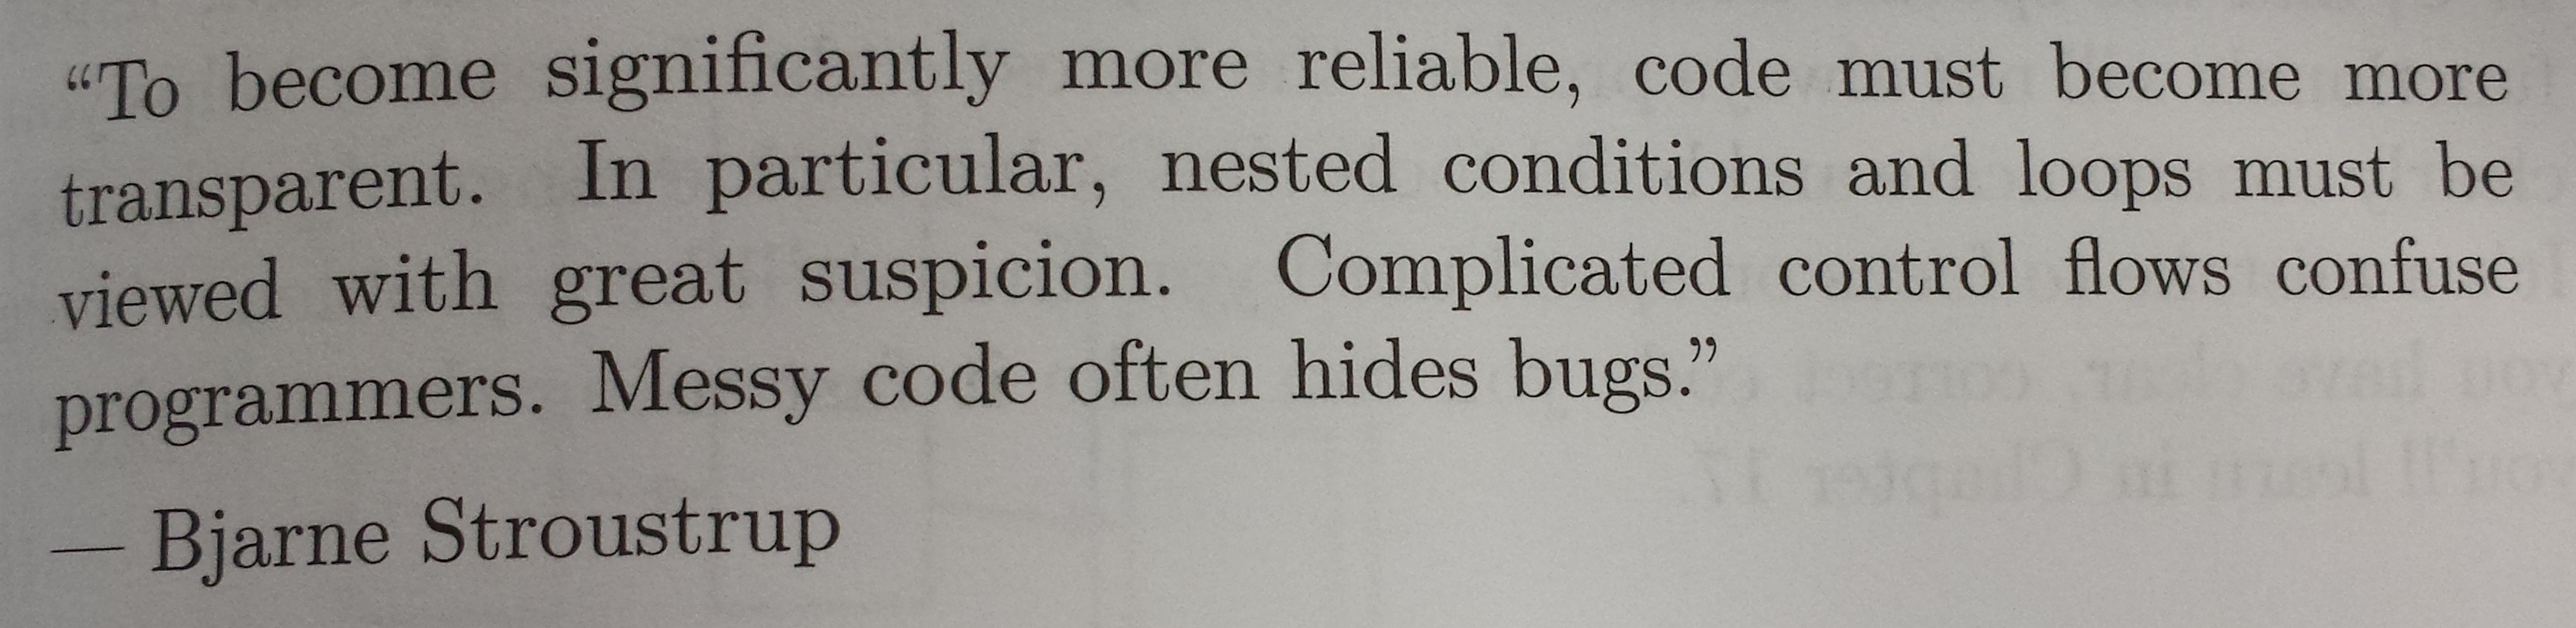
\includegraphics[width=10.56in]{images/funs} \end{center}

\subsection{Comments}\label{comments}

In code, use comments to explain the ``why'' not the ``what'' or
``how''. Each line of a comment should begin with the comment symbol and
a single space: \texttt{\#}.

\subsection{Naming}\label{naming}

\begin{quote}
There are only two hard things in Computer Science: cache invalidation
and naming things.

-- Phil Karlton
\end{quote}

Names are not limited to 8 characters as in some other languages,
however they are case sensitive. Be smart with your naming; be
descriptive yet concise. Think about how your names will show up in auto
complete.

Throughout the course we will point out some standard naming conventions
that are used in R (and other languages). (Ex. \texttt{i} and \texttt{j}
as row and column indices)

\begin{Shaded}
\begin{Highlighting}[]
\CommentTok{# Good}
\NormalTok{average_height <-}\StringTok{ }\KeywordTok{mean}\NormalTok{((feet }\OperatorTok{/}\StringTok{ }\DecValTok{12}\NormalTok{) }\OperatorTok{+}\StringTok{ }\NormalTok{inches)}
\KeywordTok{plot}\NormalTok{(mtcars}\OperatorTok{$}\NormalTok{disp, mtcars}\OperatorTok{$}\NormalTok{mpg)}

\CommentTok{# Bad}
\NormalTok{ah<-}\KeywordTok{mean}\NormalTok{(x}\OperatorTok{/}\DecValTok{12}\OperatorTok{+}\NormalTok{y)}
\KeywordTok{plot}\NormalTok{(mtcars[, }\DecValTok{3}\NormalTok{], mtcars[, }\DecValTok{1}\NormalTok{])}
\end{Highlighting}
\end{Shaded}

\subsection{Structure}\label{structure-1}

Use commented lines of \texttt{-} to create a code outline.

\subsection{Spacing}\label{spacing}

Put a space before and after \texttt{=} when naming arguments in
function calls. Most infix operators (\texttt{==}, \texttt{+},
\texttt{-}, \texttt{\textless{}-}, etc.) are also surrounded by spaces,
except those with relatively high precedence: \texttt{\^{}}, \texttt{:},
\texttt{::}, and \texttt{:::}. Always put a space after a comma, and
never before (just like in regular English).

\begin{Shaded}
\begin{Highlighting}[]
\CommentTok{# Good}
\NormalTok{average <-}\StringTok{ }\KeywordTok{mean}\NormalTok{((feet }\OperatorTok{/}\StringTok{ }\DecValTok{12}\NormalTok{) }\OperatorTok{+}\StringTok{ }\NormalTok{inches, }\DataTypeTok{na.rm =} \OtherTok{TRUE}\NormalTok{)}
\KeywordTok{sqrt}\NormalTok{(x}\OperatorTok{^}\DecValTok{2} \OperatorTok{+}\StringTok{ }\NormalTok{y}\OperatorTok{^}\DecValTok{2}\NormalTok{)}
\NormalTok{x <-}\StringTok{ }\DecValTok{1}\OperatorTok{:}\DecValTok{10}
\NormalTok{base}\OperatorTok{::}\NormalTok{sum}

\CommentTok{# Bad}
\NormalTok{average<-}\KeywordTok{mean}\NormalTok{(feet}\OperatorTok{/}\DecValTok{12}\OperatorTok{+}\NormalTok{inches,}\DataTypeTok{na.rm=}\OtherTok{TRUE}\NormalTok{)}
\KeywordTok{sqrt}\NormalTok{(x }\OperatorTok{^}\StringTok{ }\DecValTok{2} \OperatorTok{+}\StringTok{ }\NormalTok{y }\OperatorTok{^}\StringTok{ }\DecValTok{2}\NormalTok{)}
\NormalTok{x <-}\StringTok{ }\DecValTok{1} \OperatorTok{:}\StringTok{ }\DecValTok{10}
\NormalTok{base }\OperatorTok{::}\StringTok{ }\NormalTok{sum}
\end{Highlighting}
\end{Shaded}

\subsection{Indenting}\label{indenting}

Curly braces, \texttt{\{\}}, define the the most important hierarchy of
R code. To make this hierarchy easy to see, always indent the code
inside \texttt{\{\}} by two spaces.

\begin{Shaded}
\begin{Highlighting}[]
\CommentTok{# Good}
\ControlFlowTok{if}\NormalTok{ (y }\OperatorTok{<}\StringTok{ }\DecValTok{0} \OperatorTok{&&}\StringTok{ }\NormalTok{debug) \{}
  \KeywordTok{message}\NormalTok{(}\StringTok{"y is negative"}\NormalTok{)}
\NormalTok{\}}

\ControlFlowTok{if}\NormalTok{ (y }\OperatorTok{==}\StringTok{ }\DecValTok{0}\NormalTok{) \{}
  \ControlFlowTok{if}\NormalTok{ (x }\OperatorTok{>}\StringTok{ }\DecValTok{0}\NormalTok{) \{}
    \KeywordTok{log}\NormalTok{(x)}
\NormalTok{  \} }\ControlFlowTok{else}\NormalTok{ \{}
    \KeywordTok{message}\NormalTok{(}\StringTok{"x is negative or zero"}\NormalTok{)}
\NormalTok{  \}}
\NormalTok{\} }\ControlFlowTok{else}\NormalTok{ \{}
\NormalTok{  y }\OperatorTok{^}\StringTok{ }\NormalTok{x}
\NormalTok{\}}

\CommentTok{# Bad}
\ControlFlowTok{if}\NormalTok{ (y }\OperatorTok{<}\StringTok{ }\DecValTok{0} \OperatorTok{&&}\StringTok{ }\NormalTok{debug)}
\KeywordTok{message}\NormalTok{(}\StringTok{"Y is negative"}\NormalTok{)}

\ControlFlowTok{if}\NormalTok{ (y }\OperatorTok{==}\StringTok{ }\DecValTok{0}\NormalTok{)}
\NormalTok{\{}
    \ControlFlowTok{if}\NormalTok{ (x }\OperatorTok{>}\StringTok{ }\DecValTok{0}\NormalTok{) \{}
      \KeywordTok{log}\NormalTok{(x)}
\NormalTok{    \} }\ControlFlowTok{else}\NormalTok{ \{}
  \KeywordTok{message}\NormalTok{(}\StringTok{"x is negative or zero"}\NormalTok{)}
\NormalTok{    \}}
\NormalTok{\} }\ControlFlowTok{else}\NormalTok{ \{ y }\OperatorTok{^}\StringTok{ }\NormalTok{x \}}
\end{Highlighting}
\end{Shaded}

\subsection{Long lines}\label{long-lines}

Strive to limit your code to 80 characters per line. This fits
comfortably on a printed page with a reasonably sized font. If you find
yourself running out of room, this is a good indication that you should
encapsulate some of the work into a separate function.

If a function call is too long to fit on a single line, use one line
each for the function name, each argument, and the closing \texttt{)}.
This makes the code easier to read and to change later.

\begin{Shaded}
\begin{Highlighting}[]
\CommentTok{# Good}
\KeywordTok{do_something_very_complicated}\NormalTok{(}
  \DataTypeTok{something =} \StringTok{"that"}\NormalTok{,}
  \DataTypeTok{requires  =}\NormalTok{ many,}
  \DataTypeTok{arguments =} \StringTok{"some of which may be long"}
\NormalTok{)}

\CommentTok{# Bad}
\KeywordTok{do_something_very_complicated}\NormalTok{(}\StringTok{"that"}\NormalTok{, requires, many, arguments,}
                              \StringTok{"some of which may be long"}
\end{Highlighting}
\end{Shaded}

\subsection{Other}\label{other}

\begin{itemize}
\tightlist
\item
  Use \texttt{\textless{}-}, not \texttt{=}, for assignment. Keep
  \texttt{=} for parameters.
\end{itemize}

\begin{Shaded}
\begin{Highlighting}[]
\CommentTok{# Good}
\NormalTok{x <-}\StringTok{ }\DecValTok{5}
\KeywordTok{system.time}\NormalTok{(}
\NormalTok{  x <-}\StringTok{ }\KeywordTok{rnorm}\NormalTok{(}\FloatTok{1e6}\NormalTok{)}
\NormalTok{)}

\CommentTok{# Bad}
\NormalTok{x =}\StringTok{ }\DecValTok{5}
\KeywordTok{system.time}\NormalTok{(}
  \DataTypeTok{x =} \KeywordTok{rnorm}\NormalTok{(}\FloatTok{1e6}\NormalTok{)}
\NormalTok{)}
\end{Highlighting}
\end{Shaded}

\begin{itemize}
\item
  Don't put \texttt{;} at the end of a line, and don't use \texttt{;} to
  put multiple commands on one line.
\item
  Only use \texttt{return()} for early returns. Otherwise rely on R to
  return the result of the last evaluated expression.
\end{itemize}

\begin{Shaded}
\begin{Highlighting}[]
\CommentTok{# Good}
\NormalTok{add_two <-}\StringTok{ }\ControlFlowTok{function}\NormalTok{(x, y) \{}
\NormalTok{  x }\OperatorTok{+}\StringTok{ }\NormalTok{y}
\NormalTok{\}}

\CommentTok{# Bad}
\NormalTok{add_two <-}\StringTok{ }\ControlFlowTok{function}\NormalTok{(x, y) \{}
  \KeywordTok{return}\NormalTok{(x }\OperatorTok{+}\StringTok{ }\NormalTok{y)}
\NormalTok{\}}
\end{Highlighting}
\end{Shaded}

\begin{itemize}
\tightlist
\item
  Use \texttt{"}, not \texttt{\textquotesingle{}}, for quoting text. The
  only exception is when the text already contains double quotes and no
  single quotes.
\end{itemize}

\begin{Shaded}
\begin{Highlighting}[]
\CommentTok{# Good}
\StringTok{"Text"}
\StringTok{'Text with "quotes"'}
\StringTok{'<a href="http://style.tidyverse.org">A link</a>'}

\CommentTok{# Bad}
\StringTok{'Text'}
\StringTok{'Text with "double" and }\CharTok{\textbackslash{}'}\StringTok{single}\CharTok{\textbackslash{}'}\StringTok{ quotes'}
\end{Highlighting}
\end{Shaded}

\section{Coding practices}\label{coding-practices}

\subsection{Variables}\label{variables}

Create variables for values that are likely to change.

\subsection[\emph{Rule of Three}]{\texorpdfstring{\emph{Rule of
Three}\footnote{This is sometimes called the DRY principle, or Don't
  Repeat Yourself.}}{Rule of Three}}\label{rule-of-threedry}

Try not to copy code, or copy then modify the code, more than twice.

\begin{itemize}
\tightlist
\item
  If a change requires you to search/replace 3 or more times make a
  variable.
\item
  If you copy a code chunk 3 or more times \emph{make a function}
\item
  If you copy a function 3 or more times \emph{make your function more
  generic}
\item
  If you copy a function into a project 3 or more times \emph{make a
  package}
\item
  If 3 or more people will use the function \emph{make a package}
\end{itemize}

The \emph{Rule of Threee} applies look-up tables and such. The key thing
to think about is; if something changes how many touch points will there
be? If it is 3 or more places it is time to abstract this code a bit.

\subsection{Path names}\label{path-names}

It is better to use relative path names instead of hard coded ones. If
you must read from (or write to) paths that are not in your project
directory structure create a file name variable at the highest level you
can (\emph{always end with the \texttt{/}}) and then use relative
paths.\\
\textbf{DO NOT EVER USE \texttt{setwd()}}

\begin{Shaded}
\begin{Highlighting}[]
\CommentTok{# Good}
\NormalTok{raw_data <-}\StringTok{ }\KeywordTok{read.csv}\NormalTok{(}\StringTok{"./data/mydatafile.csv"}\NormalTok{) }

\NormalTok{input_file <-}\StringTok{ "./data/mydatafile.csv"}
\NormalTok{raw_data <-}\StringTok{ }\KeywordTok{read.csv}\NormalTok{(input_file)  }

\NormalTok{input_path <-}\StringTok{ "C:/Path/To/Some/other/project/directory/"}
\NormalTok{input_file <-}\StringTok{ }\KeywordTok{paste0}\NormalTok{(input_path, }\StringTok{"data/mydatafile.csv"}\NormalTok{)}
\NormalTok{raw_data <-}\StringTok{ }\KeywordTok{read.csv}\NormalTok{(input_file)}

\CommentTok{# Bad}
\KeywordTok{setwd}\NormalTok{(}\StringTok{"C:/Path/To/Some/other/project/directory/data/"}\NormalTok{)}
\NormalTok{raw_data <-}\StringTok{ }\KeywordTok{read.csv}\NormalTok{(}\StringTok{"mydatafile.csv"}\NormalTok{)}
\KeywordTok{setwd}\NormalTok{(}\StringTok{"C:/Path/back/to/my/project/"}\NormalTok{)}
\end{Highlighting}
\end{Shaded}

\section{RStudio}\label{rstudio}

Download the latest version of
\href{https://www.rstudio.com/products/rstudio/download/\#download}{RStudio}
(\textgreater{} 1.1) and use it!

Learn more about new features of RStudio v1.1
\href{https://www.rstudio.com/resources/videos/rstudio-1-1-new-features/}{there}.

RStudio features:

\begin{itemize}
\item
  everything you can expect from a good IDE
\item
  keyboard shortcuts I use frequently

  \begin{enumerate}
  \def\labelenumi{\arabic{enumi}.}
  \tightlist
  \item
    \emph{Ctrl + Space} (auto-completion, better than \emph{Tab})
  \item
    \emph{Ctrl + Up} (command history \& search)
  \item
    \emph{Ctrl + Enter} (execute line of code)
  \item
    \emph{Ctrl + Shift + A} (reformat code)
  \item
    \emph{Ctrl + Shift + C} (comment/uncomment selected lines)
  \item
    \emph{Ctrl + Shift + /} (reflow comments)
  \item
    \emph{Ctrl + Shift + O} (View code outline)
  \item
    \emph{Ctrl + Shift + B} (build package, website or book)
  \item
    \emph{Ctrl + Shift + M} (pipe)
  \item
    \emph{Alt + Shift + K} to see all shortcuts\ldots{}
  \end{enumerate}
\item
  Panels (everything is integrated, including \textbf{Git} and a
  terminal)
\item
  Interactive data importation from files and connections (see
  \href{https://www.rstudio.com/resources/webinars/importing-data-into-r/}{this
  webinar})
\item
  Use
  \href{https://support.rstudio.com/hc/en-us/articles/205753617-Code-Diagnostics}{code
  diagnostics}:
\item
  \textbf{R Projects}:

  \begin{itemize}
  \tightlist
  \item
    \textbf{Meaningful structure} in one folder
  \item
    The working directory automatically switches to the project's folder
  \item
    File tab displays the associated files and folders in the project
  \item
    History of R commands and open files
  \item
    Any settings associated with the project, such as Git settings, are
    loaded. Note that a \emph{set-up.R} or even a \emph{.Rprofile} file
    in the project's root directory enable project-specific settings to
    be loaded each time people work on the project.
  \end{itemize}
\end{itemize}

The only two things that make @JennyBryan 😤😠🤯. Instead use projects +
here::here() \#rstats pic.twitter.com/GwxnHePL4n

--- Hadley Wickham (@hadleywickham) December 11 2017

Read more at
\url{https://www.tidyverse.org/articles/2017/12/workflow-vs-script/} and
also see chapter
\href{https://bookdown.org/csgillespie/efficientR/set-up.html}{\emph{Efficient
set-up}} of book \emph{Efficient R programming}.

\section{Getting help}\label{getting-help}

\subsection{Help yourself, learn how to
debug}\label{help-yourself-learn-how-to-debug}

A basic solution is to print everything, but it usually does not work
well on complex problems. A convenient solution to see all the
variables' states in your code is to place some \texttt{browser()}
anywhere you want to check the variables' states.

Learn more with
\href{https://bookdown.org/rdpeng/rprogdatascience/debugging.html}{this
book chapter},
\href{http://adv-r.had.co.nz/Exceptions-Debugging.html}{this other book
chapter},
\href{https://www.rstudio.com/resources/videos/debugging-techniques-in-rstudio/}{this
webinar} and
\href{https://support.rstudio.com/hc/en-us/articles/205612627-Debugging-with-RStudio}{this
RStudio article}.

\subsection{External help}\label{external-help}

Can't remember useful functions? Use
\href{https://www.rstudio.com/resources/cheatsheets/}{cheat sheets}.

You can search for specific R stuff on \url{https://rseek.org/}. You
should also read documentations carefully. If you're using a package,
search for vignettes and a GitHub repository.

You can also use \href{https://stackoverflow.com/}{Stack Overflow}. The
most common use of Stack Overflow is when you have an error or a
question, you Google it, and most of the times the first links are Q/A
on Stack Overflow.

You can ask questions on Stack Overflow (using the tag \texttt{r}). You
need to
\href{https://stackoverflow.com/questions/5963269/how-to-make-a-great-r-reproducible-example}{make
a great R reproducible example} if you want your question to be
answered. Most of the times, while making this reproducible example, you
will find the answer to your problem.

If you're confident enough in your R skills, you can go to the next step
and
\href{https://stackoverflow.com/unanswered/tagged/r?tab=newest}{answer
questions on Stack Overflow}. It's a good way to increase your skills,
or just to
\href{https://privefl.github.io/blog/one-month-as-a-procrastinator-on-stack-overflow/}{procrastinate
while writing a scientific manuscript}.

\section{Keeping up to date}\label{keeping-up-to-date}

With over 10,000 packages on CRAN it is hard to keep up with the
constantly changing landscape.
\href{https://www.r-bloggers.com/}{R-Bloggers} is an R focused blog
aggregation site with dozens of posts per day. Check it out.

Join the \href{https://www.r-project.org/mail.html}{R-help} mailing
list. Sign up to get the daily digest and scan it for questions that
interest you.

\section{Exercises}\label{exercises}

\begin{enumerate}
\def\labelenumi{\arabic{enumi}.}
\tightlist
\item
  See these RStudio
  \href{https://rviews.rstudio.com/categories/tips-and-tricks/}{Tips \&
  Tricks} or \href{https://twitter.com/rstudiotips}{these} and find one
  that looks interesting and \textbf{practice} it all week.
\item
  Create an R Project for this class.
\item
  Create the following directories in your project (tip sheet?)

  \begin{itemize}
  \tightlist
  \item
    Bonus points if you can do it from R and not RStudio or Windows
    Explorer
  \item
    Double Bonus points if you can make it a function.
  \end{itemize}
\item
  Read Chapters 1-3 of the
  \href{http://style.tidyverse.org/index.html}{Tidyverse Style Guide}
\item
  Copy one of your R scripts into your R directory. (Bonus points if you
  can do it from R and not RStudio or Windows Explorer)
\item
  Apply the style guide to your code.\\
\item
  Apply the ``Rule of 3''

  \begin{itemize}
  \tightlist
  \item
    Create variables as needed
  \item
    Identify code that is used 3 or more times to make functions
  \item
    Identify code that would be useful in 3 or more projects to
    integrate into a package.
  \end{itemize}
\item
  Read how to
  \href{https://stackoverflow.com/questions/5963269/how-to-make-a-great-r-reproducible-example}{make
  a great R reproducible example}
\end{enumerate}

\part{Base R Basics}\label{part-base-r-basics}

\chapter{R Basics}\label{baser-rbasics}

With over 10,000 packages on CRAN we can't cover everything. In general
there are several ways, or packages, to accomplish a given task.

Here is a quick overview of the basics. Next we'll dive deep into R's
basic data structures and then how to subset these data structures. This
will give us a good overview of base R and the background needed to dive
into \textbf{R for Data Science}.

The three most important functions in R \texttt{?}, \texttt{??}, and
\texttt{str}:

\begin{itemize}
\tightlist
\item
  \texttt{?topic} provides access to the documentation for \emph{topic}.
\item
  \texttt{??topic} searches the documentation for \emph{topic}.
\item
  \texttt{str} displays the structure of an R object in human readable
  form.
\end{itemize}

See this \href{http://adv-r.had.co.nz/Vocabulary.html}{vocabulary list}
for a good starting point on the basics functions in base R and some
important libraries.

A book to learn the basics is
\href{https://bookdown.org/rdpeng/rprogdatascience/}{R Programmig for
Data Science}

In R there three basic constructs; objects, functions, and environments:

\section{Assignment Operators}\label{assignment-operators}

We saw this is Coding Style. Use \texttt{\textless{}-} for assignment
and use \texttt{=} for parameters. While you can use \texttt{=} for
assignment it is generally considered bad practice.

\section{Objects}\label{objects}

\subsection{Vector}\label{vector}

You create a vector with \texttt{c}.

\begin{Shaded}
\begin{Highlighting}[]
\NormalTok{v <-}\StringTok{ }\KeywordTok{c}\NormalTok{(}\StringTok{"my"}\NormalTok{, }\StringTok{"first"}\NormalTok{, }\StringTok{"vector"}\NormalTok{)}
\NormalTok{v}
\CommentTok{#> [1] "my"     "first"  "vector"}

\CommentTok{# length of our vector}
\KeywordTok{length}\NormalTok{(v)}
\CommentTok{#> [1] 3}
\end{Highlighting}
\end{Shaded}

There are several shortcut functions for common vector creation.

\begin{Shaded}
\begin{Highlighting}[]
\CommentTok{# create an ordered sequence}
\DecValTok{2}\OperatorTok{:}\DecValTok{10}
\CommentTok{#> [1]  2  3  4  5  6  7  8  9 10}
\DecValTok{9}\OperatorTok{:}\DecValTok{3}
\CommentTok{#> [1] 9 8 7 6 5 4 3}

\CommentTok{# generate regular sequences}
\KeywordTok{seq}\NormalTok{(}\DecValTok{1}\NormalTok{, }\DecValTok{20}\NormalTok{, }\DataTypeTok{by =} \DecValTok{3}\NormalTok{)}
\CommentTok{#> [1]  1  4  7 10 13 16 19}

\CommentTok{# replicate a number n times}
\KeywordTok{rep}\NormalTok{(}\DecValTok{3}\NormalTok{, }\DataTypeTok{times =} \DecValTok{4}\NormalTok{)}
\CommentTok{#> [1] 3 3 3 3}

\CommentTok{# arguments are generally vectorized}
\KeywordTok{rep}\NormalTok{(}\DecValTok{1}\OperatorTok{:}\DecValTok{3}\NormalTok{, }\DataTypeTok{times =} \DecValTok{3}\OperatorTok{:}\DecValTok{1}\NormalTok{)}
\CommentTok{#> [1] 1 1 1 2 2 3}

\CommentTok{# common mistake using 1:length(n) in loops}
\CommentTok{# but if n = 0}
\DecValTok{1}\OperatorTok{:}\DecValTok{0}
\CommentTok{#> [1] 1 0}

\CommentTok{# use seq_len(n) instead and the loop won't execute}
\KeywordTok{seq_len}\NormalTok{(}\DecValTok{0}\NormalTok{)}
\CommentTok{#> integer(0)}

\CommentTok{# another common mistake}
\NormalTok{n <-}\StringTok{ }\DecValTok{6}
\DecValTok{1}\OperatorTok{:}\NormalTok{n}\OperatorTok{+}\DecValTok{1}        \CommentTok{# is (1:n) + 1, so 2:(n + 1)}
\CommentTok{#> [1] 2 3 4 5 6 7}
\DecValTok{1}\OperatorTok{:}\NormalTok{(n}\OperatorTok{+}\DecValTok{1}\NormalTok{)      }\CommentTok{# usually what is meant}
\CommentTok{#> [1] 1 2 3 4 5 6 7}
\KeywordTok{seq_len}\NormalTok{(n}\OperatorTok{+}\DecValTok{1}\NormalTok{) }\CommentTok{# a better way}
\CommentTok{#> [1] 1 2 3 4 5 6 7}
\end{Highlighting}
\end{Shaded}

\subsection{Matrix}\label{matrix}

Matrices are 2D vectors, with all elements of the same type. Generally
used for mathematics.

\begin{Shaded}
\begin{Highlighting}[]
\CommentTok{# fill in column order (default)}
\KeywordTok{matrix}\NormalTok{(}\DecValTok{1}\OperatorTok{:}\DecValTok{12}\NormalTok{, }\DataTypeTok{nrow =} \DecValTok{3}\NormalTok{)}
\CommentTok{#>      [,1] [,2] [,3] [,4]}
\CommentTok{#> [1,]    1    4    7   10}
\CommentTok{#> [2,]    2    5    8   11}
\CommentTok{#> [3,]    3    6    9   12}

\CommentTok{# fill in row order}
\KeywordTok{matrix}\NormalTok{(}\DecValTok{1}\OperatorTok{:}\DecValTok{12}\NormalTok{, }\DataTypeTok{nrow =} \DecValTok{3}\NormalTok{, }\DataTypeTok{byrow =} \OtherTok{TRUE}\NormalTok{)}
\CommentTok{#>      [,1] [,2] [,3] [,4]}
\CommentTok{#> [1,]    1    2    3    4}
\CommentTok{#> [2,]    5    6    7    8}
\CommentTok{#> [3,]    9   10   11   12}

\CommentTok{# can also specify the number of columns instead}
\KeywordTok{matrix}\NormalTok{(}\DecValTok{1}\OperatorTok{:}\DecValTok{12}\NormalTok{, }\DataTypeTok{ncol =} \DecValTok{3}\NormalTok{)}
\CommentTok{#>      [,1] [,2] [,3]}
\CommentTok{#> [1,]    1    5    9}
\CommentTok{#> [2,]    2    6   10}
\CommentTok{#> [3,]    3    7   11}
\CommentTok{#> [4,]    4    8   12}
\end{Highlighting}
\end{Shaded}

You find the dimensions of a matrix with \texttt{nrow}, \texttt{ncol},
and \texttt{dim}

\begin{Shaded}
\begin{Highlighting}[]
\NormalTok{m <-}\StringTok{ }\KeywordTok{matrix}\NormalTok{(}\DecValTok{1}\OperatorTok{:}\DecValTok{12}\NormalTok{, }\DataTypeTok{ncol =} \DecValTok{3}\NormalTok{)}
\KeywordTok{dim}\NormalTok{(m)}
\CommentTok{#> [1] 4 3}
\KeywordTok{nrow}\NormalTok{(m)}
\CommentTok{#> [1] 4}
\KeywordTok{ncol}\NormalTok{(m)}
\CommentTok{#> [1] 3}
\end{Highlighting}
\end{Shaded}

\subsection{List}\label{list}

A list is a generic vector containing other objects. These do
\textbf{NOT} have to be the same type or the same length.

\begin{Shaded}
\begin{Highlighting}[]
\NormalTok{s <-}\StringTok{ }\KeywordTok{c}\NormalTok{(}\StringTok{"aa"}\NormalTok{, }\StringTok{"bb"}\NormalTok{, }\StringTok{"cc"}\NormalTok{, }\StringTok{"dd"}\NormalTok{, }\StringTok{"ee"}\NormalTok{) }
\NormalTok{b <-}\StringTok{ }\KeywordTok{c}\NormalTok{(}\OtherTok{TRUE}\NormalTok{, }\OtherTok{FALSE}\NormalTok{, }\OtherTok{TRUE}\NormalTok{, }\OtherTok{FALSE}\NormalTok{, }\OtherTok{FALSE}\NormalTok{) }
\CommentTok{# x contains copies of n, s, b and our matrix from above}
\NormalTok{x <-}\StringTok{ }\KeywordTok{list}\NormalTok{(}\DataTypeTok{n =} \KeywordTok{c}\NormalTok{(}\DecValTok{2}\NormalTok{, }\DecValTok{3}\NormalTok{, }\DecValTok{5}\NormalTok{) , s, b, }\DecValTok{3}\NormalTok{, m)   }
\NormalTok{x}
\CommentTok{#> $n}
\CommentTok{#> [1] 2 3 5}
\CommentTok{#> }
\CommentTok{#> [[2]]}
\CommentTok{#> [1] "aa" "bb" "cc" "dd" "ee"}
\CommentTok{#> }
\CommentTok{#> [[3]]}
\CommentTok{#> [1]  TRUE FALSE  TRUE FALSE FALSE}
\CommentTok{#> }
\CommentTok{#> [[4]]}
\CommentTok{#> [1] 3}
\CommentTok{#> }
\CommentTok{#> [[5]]}
\CommentTok{#>      [,1] [,2] [,3]}
\CommentTok{#> [1,]    1    5    9}
\CommentTok{#> [2,]    2    6   10}
\CommentTok{#> [3,]    3    7   11}
\CommentTok{#> [4,]    4    8   12}

\CommentTok{# length gives you length of the list not the elements in the list}
\KeywordTok{length}\NormalTok{(x)}
\CommentTok{#> [1] 5}
\end{Highlighting}
\end{Shaded}

We'll discuss lists in detail in the next chapter.

\subsection{Data frame}\label{data-frame}

A data frame is a list with each vector of the same length. This is the
main data structure used and is analogous to a data set in SAS. While
these \textbf{look} like matrices they behave very different.

\begin{Shaded}
\begin{Highlighting}[]
\NormalTok{df =}\StringTok{ }\KeywordTok{data.frame}\NormalTok{(}\DataTypeTok{n =} \KeywordTok{c}\NormalTok{(}\DecValTok{2}\NormalTok{, }\DecValTok{3}\NormalTok{, }\DecValTok{5}\NormalTok{),}
                \DataTypeTok{s =} \KeywordTok{c}\NormalTok{(}\StringTok{"aa"}\NormalTok{, }\StringTok{"bb"}\NormalTok{, }\StringTok{"cc"}\NormalTok{),}
                \DataTypeTok{b =} \KeywordTok{c}\NormalTok{(}\OtherTok{TRUE}\NormalTok{, }\OtherTok{FALSE}\NormalTok{, }\OtherTok{TRUE}\NormalTok{),}
                \DataTypeTok{y =}\NormalTok{ v}
\NormalTok{                )       }\CommentTok{# df is a data frame }
\NormalTok{df}
\CommentTok{#>   n  s     b      y}
\CommentTok{#> 1 2 aa  TRUE     my}
\CommentTok{#> 2 3 bb FALSE  first}
\CommentTok{#> 3 5 cc  TRUE vector}

\CommentTok{# dimensions}
\KeywordTok{dim}\NormalTok{(df)}
\CommentTok{#> [1] 3 4}
\KeywordTok{nrow}\NormalTok{(df)}
\CommentTok{#> [1] 3}
\KeywordTok{ncol}\NormalTok{(df)}
\CommentTok{#> [1] 4}
\KeywordTok{length}\NormalTok{(df)}
\CommentTok{#> [1] 4}
\end{Highlighting}
\end{Shaded}

We'll discuss data frames in greater detail in the next chapter.

\section{Comparision}\label{comparision}

Logical Operators include:

\begin{longtable}[]{@{}ll@{}}
\toprule
Operator & Description\tabularnewline
\midrule
\endhead
\textgreater{} & greater than\tabularnewline
\textgreater{}= & greater than or equal to\tabularnewline
\textless{} & less than\tabularnewline
\textless{}= & less than or equal to\tabularnewline
== & exactly equal to\tabularnewline
!= & not equal to\tabularnewline
\bottomrule
\end{longtable}

\begin{Shaded}
\begin{Highlighting}[]
\NormalTok{v <-}\StringTok{ }\DecValTok{1}\OperatorTok{:}\DecValTok{12}
\NormalTok{v[v }\OperatorTok{>}\StringTok{ }\DecValTok{9}\NormalTok{]}
\CommentTok{#> [1] 10 11 12}
\end{Highlighting}
\end{Shaded}

Equality can be tricky to test for since real numbers can't be expressed
exactly in computers.

\begin{Shaded}
\begin{Highlighting}[]
\NormalTok{x <-}\StringTok{ }\KeywordTok{sqrt}\NormalTok{(}\DecValTok{2}\NormalTok{)}
\NormalTok{(y <-}\StringTok{ }\NormalTok{x}\OperatorTok{^}\DecValTok{2}\NormalTok{)}
\CommentTok{#> [1] 2}
\NormalTok{y }\OperatorTok{==}\StringTok{ }\DecValTok{2}
\CommentTok{#> [1] FALSE}
\KeywordTok{print}\NormalTok{(y, }\DataTypeTok{digits =} \DecValTok{20}\NormalTok{)}
\CommentTok{#> [1] 2.0000000000000004}
\KeywordTok{all.equal}\NormalTok{(y, }\DecValTok{2}\NormalTok{)          ## equality with some tolerance}
\CommentTok{#> [1] TRUE}
\KeywordTok{all.equal}\NormalTok{(y, }\DecValTok{3}\NormalTok{)}
\CommentTok{#> [1] "Mean relative difference: 0.5"}
\KeywordTok{isTRUE}\NormalTok{(}\KeywordTok{all.equal}\NormalTok{(y, }\DecValTok{3}\NormalTok{))  ## if you want a boolean, use isTRUE()}
\CommentTok{#> [1] FALSE}
\end{Highlighting}
\end{Shaded}

\section{Logical and sets}\label{logical-and-sets}

\begin{Shaded}
\begin{Highlighting}[]
\NormalTok{x <-}\StringTok{ }\KeywordTok{c}\NormalTok{(}\OtherTok{TRUE}\NormalTok{, }\OtherTok{FALSE}\NormalTok{)}
\NormalTok{df <-}\StringTok{ }\KeywordTok{data.frame}\NormalTok{(}\KeywordTok{expand.grid}\NormalTok{(x, x))}
\KeywordTok{names}\NormalTok{(df) <-}\StringTok{ }\KeywordTok{c}\NormalTok{(}\StringTok{"x"}\NormalTok{, }\StringTok{"y"}\NormalTok{)}
\NormalTok{df}\OperatorTok{$}\NormalTok{and  <-}\StringTok{ }\NormalTok{df}\OperatorTok{$}\NormalTok{x }\OperatorTok{&}\StringTok{ }\NormalTok{df}\OperatorTok{$}\NormalTok{y     }\CommentTok{# logical and}
\NormalTok{df}\OperatorTok{$}\NormalTok{or   <-}\StringTok{ }\NormalTok{df}\OperatorTok{$}\NormalTok{x }\OperatorTok{|}\StringTok{ }\NormalTok{df}\OperatorTok{$}\NormalTok{y     }\CommentTok{# logical or}
\NormalTok{df}\OperatorTok{$}\NormalTok{notx <-}\StringTok{ }\OperatorTok{!}\NormalTok{df}\OperatorTok{$}\NormalTok{x           }\CommentTok{# negation}
\NormalTok{df}\OperatorTok{$}\NormalTok{xor  <-}\StringTok{ }\KeywordTok{xor}\NormalTok{(df}\OperatorTok{$}\NormalTok{x, df}\OperatorTok{$}\NormalTok{y) }\CommentTok{# exlusive or}
\NormalTok{df}
\CommentTok{#>       x     y   and    or  notx   xor}
\CommentTok{#> 1  TRUE  TRUE  TRUE  TRUE FALSE FALSE}
\CommentTok{#> 2 FALSE  TRUE FALSE  TRUE  TRUE  TRUE}
\CommentTok{#> 3  TRUE FALSE FALSE  TRUE FALSE  TRUE}
\CommentTok{#> 4 FALSE FALSE FALSE FALSE  TRUE FALSE}
\end{Highlighting}
\end{Shaded}

R has two versions of the logical operators \texttt{\&} and
\texttt{\&\&} (\texttt{\textbar{}} and \texttt{\textbar{}\textbar{}}).
The single version is the vectorized version while the the double
version returns a length-one vector. Use the double version in logical
control structures (if, for, while, etc).

\begin{Shaded}
\begin{Highlighting}[]
\CommentTok{# TRUE/FALSE and each element}
\OtherTok{TRUE} \OperatorTok{&}\StringTok{ }\KeywordTok{c}\NormalTok{(}\OtherTok{TRUE}\NormalTok{, }\OtherTok{FALSE}\NormalTok{)}
\CommentTok{#> [1]  TRUE FALSE}
\OtherTok{FALSE} \OperatorTok{&}\StringTok{ }\KeywordTok{c}\NormalTok{(}\OtherTok{TRUE}\NormalTok{, }\OtherTok{FALSE}\NormalTok{)}
\CommentTok{#> [1] FALSE FALSE}
\CommentTok{# TRUE/FALSE and first element}
\OtherTok{TRUE} \OperatorTok{&&}\StringTok{ }\KeywordTok{c}\NormalTok{(}\OtherTok{TRUE}\NormalTok{, }\OtherTok{FALSE}\NormalTok{)}
\CommentTok{#> [1] TRUE}
\OtherTok{FALSE} \OperatorTok{&&}\StringTok{ }\KeywordTok{c}\NormalTok{(}\OtherTok{TRUE}\NormalTok{, }\OtherTok{FALSE}\NormalTok{)}
\CommentTok{#> [1] FALSE}
\CommentTok{# TRUE/FALSE or each element}
\OtherTok{TRUE} \OperatorTok{|}\StringTok{ }\KeywordTok{c}\NormalTok{(}\OtherTok{TRUE}\NormalTok{, }\OtherTok{FALSE}\NormalTok{)}
\CommentTok{#> [1] TRUE TRUE}
\OtherTok{FALSE} \OperatorTok{|}\StringTok{ }\KeywordTok{c}\NormalTok{(}\OtherTok{TRUE}\NormalTok{, }\OtherTok{FALSE}\NormalTok{)}
\CommentTok{#> [1]  TRUE FALSE}
\CommentTok{# TRUE/FALSE or first element}
\OtherTok{TRUE} \OperatorTok{||}\StringTok{ }\KeywordTok{c}\NormalTok{(}\OtherTok{TRUE}\NormalTok{, }\OtherTok{FALSE}\NormalTok{)}
\CommentTok{#> [1] TRUE}
\OtherTok{FALSE} \OperatorTok{||}\StringTok{ }\KeywordTok{c}\NormalTok{(}\OtherTok{TRUE}\NormalTok{, }\OtherTok{FALSE}\NormalTok{)}
\CommentTok{#> [1] TRUE}
\end{Highlighting}
\end{Shaded}

This is a common source of bugs in control structures (if, for, while,
etc) where you must have a single TRUE / FALSE.

Also, note that \texttt{=} is used for assignment and not comparison
\texttt{==}.

It also has useful helpers \texttt{any} and \texttt{all}

\begin{Shaded}
\begin{Highlighting}[]
\NormalTok{x <-}\StringTok{ }\KeywordTok{c}\NormalTok{(}\OtherTok{FALSE}\NormalTok{, }\OtherTok{FALSE}\NormalTok{, }\OtherTok{FALSE}\NormalTok{, }\OtherTok{TRUE}\NormalTok{)}
\KeywordTok{any}\NormalTok{(x)}
\CommentTok{#> [1] TRUE}
\KeywordTok{all}\NormalTok{(x)}
\CommentTok{#> [1] FALSE}
\KeywordTok{all}\NormalTok{(}\OperatorTok{!}\NormalTok{x[}\DecValTok{1}\OperatorTok{:}\DecValTok{3}\NormalTok{])}
\CommentTok{#> [1] TRUE}
\end{Highlighting}
\end{Shaded}

And also some useful \textbf{set} operations \texttt{intersect},
\texttt{union}, \texttt{setdiff}, \texttt{setequal}

\begin{Shaded}
\begin{Highlighting}[]
\NormalTok{x <-}\StringTok{ }\DecValTok{1}\OperatorTok{:}\DecValTok{5}
\NormalTok{y <-}\StringTok{ }\DecValTok{3}\OperatorTok{:}\DecValTok{7}

\KeywordTok{intersect}\NormalTok{(x, y) }\CommentTok{# in x and in y}
\CommentTok{#> [1] 3 4 5}
\KeywordTok{union}\NormalTok{(x, y)     }\CommentTok{# different than c()}
\CommentTok{#> [1] 1 2 3 4 5 6 7}
\KeywordTok{c}\NormalTok{(x,y)          }\CommentTok{# not a set operation}
\CommentTok{#>  [1] 1 2 3 4 5 3 4 5 6 7}
\KeywordTok{setdiff}\NormalTok{(x, y)   }\CommentTok{# in x but not in y}
\CommentTok{#> [1] 1 2}
\KeywordTok{setdiff}\NormalTok{(y, x)   }\CommentTok{# in y but not in x}
\CommentTok{#> [1] 6 7}
\KeywordTok{setequal}\NormalTok{(x, y)}
\CommentTok{#> [1] FALSE}
\NormalTok{z <-}\StringTok{ }\DecValTok{5}\OperatorTok{:}\DecValTok{1}
\KeywordTok{setequal}\NormalTok{(x, z)}
\CommentTok{#> [1] TRUE}
\end{Highlighting}
\end{Shaded}

\section{Control Structures}\label{control-structures}

Control structures allow you to put some ``logic'' into your R code,
rather than just always executing the same R code every time. Control
structures allow you to respond to inputs or to features of the data and
execute different R expressions accordingly.

Commonly used control structures are

\begin{itemize}
\item
  \texttt{if} and \texttt{else}: testing a condition and acting on it
\item
  \texttt{for}: execute a loop a fixed number of times
\item
  \texttt{while}: execute a loop \emph{while} a condition is true
\item
  \texttt{repeat}: execute an infinite loop (must \texttt{break} out of
  it to stop)
\item
  \texttt{break}: break the execution of a loop
\item
  \texttt{next}: skip an iteration of a loop
\end{itemize}

\subsection{\texorpdfstring{\texttt{if}-\texttt{else}}{if-else}}\label{if-else}

The \texttt{if}-\texttt{else} combination is probably the most commonly
used control structure in R (or perhaps any language). This structure
allows you to test a condition and act on it depending on whether it's
true or false.

For starters, you can just use the \texttt{if} statement.

\begin{Shaded}
\begin{Highlighting}[]
\ControlFlowTok{if}\NormalTok{(}\OperatorTok{<}\NormalTok{condition}\OperatorTok{>}\NormalTok{) \{}
        \CommentTok{# do something}
\NormalTok{\} }
\CommentTok{# Continue with rest of code}
\end{Highlighting}
\end{Shaded}

The above code does nothing if the condition is false. If you have an
action you want to execute when the condition is false, then you need an
\texttt{else} clause.

\begin{Shaded}
\begin{Highlighting}[]
\ControlFlowTok{if}\NormalTok{(}\OperatorTok{<}\NormalTok{condition}\OperatorTok{>}\NormalTok{) \{}
        \CommentTok{# do something}
\NormalTok{\} }
\ControlFlowTok{else}\NormalTok{ \{}
        \CommentTok{# do something else}
\NormalTok{\}}
\end{Highlighting}
\end{Shaded}

You can have a series of tests by following the initial \texttt{if} with
any number of \texttt{else\ if}s.

\begin{Shaded}
\begin{Highlighting}[]
\ControlFlowTok{if}\NormalTok{(}\OperatorTok{<}\NormalTok{condition1}\OperatorTok{>}\NormalTok{) \{}
        \CommentTok{# do something}
\NormalTok{\} }\ControlFlowTok{else} \ControlFlowTok{if}\NormalTok{(}\OperatorTok{<}\NormalTok{condition2}\OperatorTok{>}\NormalTok{)  \{}
        \CommentTok{# do something different}
\NormalTok{\} }\ControlFlowTok{else}\NormalTok{ \{}
        \CommentTok{# do something else different}
\NormalTok{\}}
\end{Highlighting}
\end{Shaded}

\subsection{\texorpdfstring{\texttt{for}
Loops}{for Loops}}\label{for-loops}

For loops are pretty much the only looping construct that you will need
in R. While you may occasionally find a need for other types of loops,
in my experience doing data analysis, I've found very few situations
where a for loop wasn't sufficient.

In R, for loops take an iterator variable and assign it successive
values from a sequence or vector. For loops are most commonly used for
iterating over the elements of an object (list, vector, etc.)

The following three loops all have the similar behavior.

\begin{Shaded}
\begin{Highlighting}[]
\NormalTok{x <-}\StringTok{ }\KeywordTok{c}\NormalTok{(}\StringTok{"a"}\NormalTok{, }\StringTok{"b"}\NormalTok{, }\StringTok{"c"}\NormalTok{, }\StringTok{"d"}\NormalTok{)}

\ControlFlowTok{for}\NormalTok{(i }\ControlFlowTok{in} \DecValTok{1}\OperatorTok{:}\KeywordTok{length}\NormalTok{(x)) \{}
\NormalTok{        ## Print out each element of 'x'}
        \KeywordTok{print}\NormalTok{(x[i])  }
\NormalTok{\}}
\CommentTok{#> [1] "a"}
\CommentTok{#> [1] "b"}
\CommentTok{#> [1] "c"}
\CommentTok{#> [1] "d"}
\end{Highlighting}
\end{Shaded}

The \texttt{seq\_along()} function is commonly used in conjunction with
for loops in order to generate an integer sequence based on the length
of an object (in this case, the object \texttt{x}).

\begin{Shaded}
\begin{Highlighting}[]
\NormalTok{## Generate a sequence based on length of 'x'}
\ControlFlowTok{for}\NormalTok{(i }\ControlFlowTok{in} \KeywordTok{seq_along}\NormalTok{(x)) \{   }
        \KeywordTok{print}\NormalTok{(x[i])}
\NormalTok{\}}
\CommentTok{#> [1] "a"}
\CommentTok{#> [1] "b"}
\CommentTok{#> [1] "c"}
\CommentTok{#> [1] "d"}
\end{Highlighting}
\end{Shaded}

It is not necessary to use an index-type variable.

\begin{Shaded}
\begin{Highlighting}[]
\ControlFlowTok{for}\NormalTok{(letter }\ControlFlowTok{in}\NormalTok{ x) \{}
        \KeywordTok{print}\NormalTok{(letter)}
\NormalTok{\}}
\CommentTok{#> [1] "a"}
\CommentTok{#> [1] "b"}
\CommentTok{#> [1] "c"}
\CommentTok{#> [1] "d"}
\end{Highlighting}
\end{Shaded}

Nested loops are commonly needed for multidimensional or hierarchical
data structures (e.g.~matrices, lists). Be careful with nesting though.
Nesting beyond 2 to 3 levels often makes it difficult to read/understand
the code. If you find yourself in need of a large number of nested
loops, you may want to break up the loops by using functions (discussed
later).

\subsection{\texorpdfstring{\texttt{while}
Loops}{while Loops}}\label{while-loops}

While loops begin by testing a condition. If it is true, then they
execute the loop body. Once the loop body is executed, the condition is
tested again, and so forth, until the condition is false, after which
the loop exits.

\begin{Shaded}
\begin{Highlighting}[]
\NormalTok{count <-}\StringTok{ }\DecValTok{0}
\ControlFlowTok{while}\NormalTok{(count }\OperatorTok{<}\StringTok{ }\DecValTok{10}\NormalTok{) \{}
        \KeywordTok{print}\NormalTok{(count)}
\NormalTok{        count <-}\StringTok{ }\NormalTok{count }\OperatorTok{+}\StringTok{ }\DecValTok{1}
\NormalTok{\}}
\CommentTok{#> [1] 0}
\CommentTok{#> [1] 1}
\CommentTok{#> [1] 2}
\CommentTok{#> [1] 3}
\CommentTok{#> [1] 4}
\CommentTok{#> [1] 5}
\CommentTok{#> [1] 6}
\CommentTok{#> [1] 7}
\CommentTok{#> [1] 8}
\CommentTok{#> [1] 9}
\end{Highlighting}
\end{Shaded}

While loops can potentially result in infinite loops if not written
properly. Use with care!

Sometimes there will be more than one condition in the test.

\begin{Shaded}
\begin{Highlighting}[]
\NormalTok{z <-}\StringTok{ }\DecValTok{5}
\KeywordTok{set.seed}\NormalTok{(}\DecValTok{1}\NormalTok{)}

\ControlFlowTok{while}\NormalTok{(z }\OperatorTok{>=}\StringTok{ }\DecValTok{3} \OperatorTok{&&}\StringTok{ }\NormalTok{z }\OperatorTok{<=}\StringTok{ }\DecValTok{10}\NormalTok{) \{}
\NormalTok{        coin <-}\StringTok{ }\KeywordTok{rbinom}\NormalTok{(}\DecValTok{1}\NormalTok{, }\DecValTok{1}\NormalTok{, }\FloatTok{0.5}\NormalTok{)}
        
        \ControlFlowTok{if}\NormalTok{(coin }\OperatorTok{==}\StringTok{ }\DecValTok{1}\NormalTok{) \{  ## random walk}
\NormalTok{                z <-}\StringTok{ }\NormalTok{z }\OperatorTok{+}\StringTok{ }\DecValTok{1}
\NormalTok{        \} }\ControlFlowTok{else}\NormalTok{ \{}
\NormalTok{                z <-}\StringTok{ }\NormalTok{z }\OperatorTok{-}\StringTok{ }\DecValTok{1}
\NormalTok{        \} }
\NormalTok{\}}
\KeywordTok{print}\NormalTok{(z)}
\CommentTok{#> [1] 2}
\end{Highlighting}
\end{Shaded}

Conditions are always evaluated from left to right. For example, in the
above code, if \texttt{z} were less than 3, the second test would not
have been evaluated.

\subsection{\texorpdfstring{\texttt{repeat}
Loops}{repeat Loops}}\label{repeat-loops}

\texttt{repeat} initiates an infinite loop right from the start. These
are not commonly used in statistical or data analysis applications but
they do have their uses. The only way to exit a \texttt{repeat} loop is
to call \texttt{break}.

One possible paradigm might be in an iterative algorithm where you may
be searching for a solution and you don't want to stop until you're
close enough to the solution. In this kind of situation, you often don't
know in advance how many iterations it's going to take to get ``close
enough'' to the solution.

\begin{Shaded}
\begin{Highlighting}[]
\NormalTok{x0 <-}\StringTok{ }\DecValTok{1}
\NormalTok{tol <-}\StringTok{ }\FloatTok{1e-8}

\ControlFlowTok{repeat}\NormalTok{ \{}
\NormalTok{        x1 <-}\StringTok{ }\KeywordTok{computeEstimate}\NormalTok{()}
        
        \ControlFlowTok{if}\NormalTok{(}\KeywordTok{abs}\NormalTok{(x1 }\OperatorTok{-}\StringTok{ }\NormalTok{x0) }\OperatorTok{<}\StringTok{ }\NormalTok{tol) \{  ## Close enough?}
                \ControlFlowTok{break}
\NormalTok{        \} }\ControlFlowTok{else}\NormalTok{ \{}
\NormalTok{                x0 <-}\StringTok{ }\NormalTok{x1}
\NormalTok{        \} }
\NormalTok{\}}
\end{Highlighting}
\end{Shaded}

Note that the above code will not run if the \texttt{computeEstimate()}
function is not defined (I just made it up for the purposes of this
demonstration).

The loop above is a bit dangerous because there's no guarantee it will
ever stop. You could get in a situation where the values of \texttt{x0}
and \texttt{x1} oscillate back and forth and never converge. Better to
set a hard limit on the number of iterations by using a \texttt{for}
loop and then report whether convergence was achieved or not.

\subsection{\texorpdfstring{\texttt{next},
\texttt{break}}{next, break}}\label{next-break}

While not used very often it's nice to know about these.

\texttt{next} is used to skip an iteration of a loop.

\begin{Shaded}
\begin{Highlighting}[]
\ControlFlowTok{for}\NormalTok{(i }\ControlFlowTok{in} \DecValTok{1}\OperatorTok{:}\DecValTok{100}\NormalTok{) \{}
        \ControlFlowTok{if}\NormalTok{(i }\OperatorTok{<=}\StringTok{ }\DecValTok{20}\NormalTok{) \{}
\NormalTok{                ## Skip the first 20 iterations}
                \ControlFlowTok{next}                 
\NormalTok{        \}}
\NormalTok{        ## Do something here}
\NormalTok{\}}
\end{Highlighting}
\end{Shaded}

\texttt{break} is used to exit a loop immediately, regardless of what
iteration the loop may be on.

\begin{Shaded}
\begin{Highlighting}[]
\ControlFlowTok{for}\NormalTok{(i }\ControlFlowTok{in} \DecValTok{1}\OperatorTok{:}\DecValTok{100}\NormalTok{) \{}
      \KeywordTok{print}\NormalTok{(i)}

      \ControlFlowTok{if}\NormalTok{(i }\OperatorTok{>}\StringTok{ }\DecValTok{20}\NormalTok{) \{}
\NormalTok{              ## Stop loop after 20 iterations}
              \ControlFlowTok{break}  
\NormalTok{      \}     }
\NormalTok{\}}
\end{Highlighting}
\end{Shaded}

\subsection{Looping}\label{looping}

For loops are so common that that R has some functions which implement
looping in a compact form to make your life easier. For a more in depth
look see
\href{https://bookdown.org/rdpeng/rprogdatascience/loop-functions.html}{this}

\begin{itemize}
\tightlist
\item
  \texttt{apply} is generic: applies a function to a matrix's rows or
  columns (or, more generally, to dimensions of an array)
\item
  \texttt{lapply} is a list apply which acts on a list or vector and
  returns a list.
\item
  \texttt{sapply} is a simple lapply but defaults to returning a vector
  (or matrix) if possible.
\item
  \texttt{vapply} is a verified apply. This is a sapply with the return
  object type prespecified.
\item
  \texttt{rapply} is a recursive apply for nested lists, i.e.~lists
  within lists
\item
  \texttt{tapply} is a tagged apply where the tags identify the subsets
  to apply a function
\item
  \texttt{mapply} is a multivariate apply for functions that have
  multiple arguments.
\item
  \texttt{Map} is a wrapper to mapply with SIMPLIFY = FALSE, so it is
  guaranteed to return a list.
\item
  \texttt{replicate} is a wrapper around sapply for repeated evaluation
  of an expression
\end{itemize}

\begin{Shaded}
\begin{Highlighting}[]
\CommentTok{# Two dimensional matrix}
\NormalTok{M <-}\StringTok{ }\KeywordTok{matrix}\NormalTok{(}\KeywordTok{sample}\NormalTok{(}\DecValTok{1}\OperatorTok{:}\DecValTok{16}\NormalTok{), }\DecValTok{4}\NormalTok{, }\DecValTok{4}\NormalTok{)}
\NormalTok{M}
\CommentTok{#>      [,1] [,2] [,3] [,4]}
\CommentTok{#> [1,]   10    9    4   14}
\CommentTok{#> [2,]    8   12    6   16}
\CommentTok{#> [3,]    3    2   15    5}
\CommentTok{#> [4,]   11    7   13    1}
\CommentTok{# apply min to rows}
\KeywordTok{apply}\NormalTok{(M, }\DecValTok{1}\NormalTok{, min)}
\CommentTok{#> [1] 4 6 2 1}
\CommentTok{# apply max to columns}
\KeywordTok{apply}\NormalTok{(M, }\DecValTok{2}\NormalTok{, max)}
\CommentTok{#> [1] 11 12 15 16}
\end{Highlighting}
\end{Shaded}

If you want row/column means or sums for a 2D matrix, be sure to
investigate the highly optimized, lightning-quick \texttt{colMeans},
\texttt{rowMeans}, \texttt{colSums}, \texttt{rowSums}.

\begin{Shaded}
\begin{Highlighting}[]
\NormalTok{x <-}\StringTok{ }\KeywordTok{list}\NormalTok{(}\DataTypeTok{a =} \DecValTok{1}\NormalTok{, }\DataTypeTok{b =} \DecValTok{1}\OperatorTok{:}\DecValTok{3}\NormalTok{, }\DataTypeTok{c =} \DecValTok{10}\OperatorTok{:}\DecValTok{25}\NormalTok{)}
\NormalTok{x}
\CommentTok{#> $a}
\CommentTok{#> [1] 1}
\CommentTok{#> }
\CommentTok{#> $b}
\CommentTok{#> [1] 1 2 3}
\CommentTok{#> }
\CommentTok{#> $c}
\CommentTok{#>  [1] 10 11 12 13 14 15 16 17 18 19 20 21 22 23 24 25}
\KeywordTok{lapply}\NormalTok{(x, }\DataTypeTok{FUN =}\NormalTok{ length) }
\CommentTok{#> $a}
\CommentTok{#> [1] 1}
\CommentTok{#> }
\CommentTok{#> $b}
\CommentTok{#> [1] 3}
\CommentTok{#> }
\CommentTok{#> $c}
\CommentTok{#> [1] 16}
\KeywordTok{sapply}\NormalTok{(x, }\DataTypeTok{FUN =}\NormalTok{ length) }
\CommentTok{#>  a  b  c }
\CommentTok{#>  1  3 16}
\KeywordTok{vapply}\NormalTok{(x, }\DataTypeTok{FUN =}\NormalTok{ length, }\DataTypeTok{FUN.VALUE =}\NormalTok{ 0L) }
\CommentTok{#>  a  b  c }
\CommentTok{#>  1  3 16}

\NormalTok{x <-}\StringTok{ }\DecValTok{1}\OperatorTok{:}\DecValTok{20}
\NormalTok{y <-}\StringTok{ }\KeywordTok{factor}\NormalTok{(}\KeywordTok{rep}\NormalTok{(letters[}\DecValTok{1}\OperatorTok{:}\DecValTok{5}\NormalTok{], }\DataTypeTok{each =} \DecValTok{4}\NormalTok{)) }\CommentTok{# a vector of the same length as x}
\KeywordTok{tapply}\NormalTok{(x, y, sum) }
\CommentTok{#>  a  b  c  d  e }
\CommentTok{#> 10 26 42 58 74}

\CommentTok{# Sums the 1st elements, the 2nd elements, etc. }
\KeywordTok{mapply}\NormalTok{(sum, }\DecValTok{1}\OperatorTok{:}\DecValTok{5}\NormalTok{, }\DecValTok{1}\OperatorTok{:}\DecValTok{5}\NormalTok{, }\DecValTok{1}\OperatorTok{:}\DecValTok{5}\NormalTok{) }
\CommentTok{#> [1]  3  6  9 12 15}

\CommentTok{# find the mean of 10 random normal variables, 5 times}
\KeywordTok{replicate}\NormalTok{(}\DecValTok{5}\NormalTok{, }\KeywordTok{mean}\NormalTok{(}\KeywordTok{rnorm}\NormalTok{(}\DecValTok{10}\NormalTok{)))}
\CommentTok{#> [1] -0.2258  0.4434 -0.0499 -0.3555 -0.1810}
\end{Highlighting}
\end{Shaded}

\texttt{tapply} is in a simalar spirit to a common data analysis
paradigm called split-apply-combine where we split our data set based on
a group, apply a function or code to it, and combine the results back
together. We will revisit this paradigm in greater detail when we get to
\emph{R for Data Science}.

\section{Vectorization \& Recycling}\label{vectorization-recycling}

Many operations in R are \emph{vectorized}, meaning that operations
occur in parallel in certain R objects. This allows you to write code
that is efficient, concise, and easier to read than in non-vectorized
languages.

The simplest example is when adding two vectors together.

\begin{Shaded}
\begin{Highlighting}[]
\NormalTok{x <-}\StringTok{ }\DecValTok{1}\OperatorTok{:}\DecValTok{3}
\NormalTok{y <-}\StringTok{ }\DecValTok{11}\OperatorTok{:}\DecValTok{13}
\NormalTok{z <-}\StringTok{ }\NormalTok{x }\OperatorTok{+}\StringTok{ }\NormalTok{y}
\NormalTok{z}
\CommentTok{#> [1] 12 14 16}
\end{Highlighting}
\end{Shaded}

In most other languages you would have to do something like

\begin{Shaded}
\begin{Highlighting}[]
\NormalTok{z <-}\StringTok{ }\KeywordTok{numeric}\NormalTok{(}\KeywordTok{length}\NormalTok{(x))}

\ControlFlowTok{for}\NormalTok{(i }\ControlFlowTok{in} \KeywordTok{seq_along}\NormalTok{(x)) \{}
\NormalTok{      z[i] <-}\StringTok{ }\NormalTok{x[i] }\OperatorTok{+}\StringTok{ }\NormalTok{y[i]}
\NormalTok{\}}
\NormalTok{z}
\CommentTok{#> [1] 12 14 16}
\end{Highlighting}
\end{Shaded}

We saw a a form of vectorization above in the logical operators.

\begin{Shaded}
\begin{Highlighting}[]
\NormalTok{x}
\CommentTok{#> [1] 1 2 3}
\NormalTok{x }\OperatorTok{>}\StringTok{ }\DecValTok{2}
\CommentTok{#> [1] FALSE FALSE  TRUE}
\NormalTok{x[x }\OperatorTok{>}\StringTok{ }\DecValTok{2}\NormalTok{]}
\CommentTok{#> [1] 3}
\end{Highlighting}
\end{Shaded}

Matrix operations are also vectorized, making for nice compact notation.
This way, we can do element-by-element operations on matrices without
having to loop over every element.

\begin{Shaded}
\begin{Highlighting}[]
\NormalTok{x <-}\StringTok{ }\KeywordTok{matrix}\NormalTok{(}\DecValTok{1}\OperatorTok{:}\DecValTok{4}\NormalTok{, }\DecValTok{2}\NormalTok{, }\DecValTok{2}\NormalTok{)}
\NormalTok{y <-}\StringTok{ }\KeywordTok{matrix}\NormalTok{(}\KeywordTok{rep}\NormalTok{(}\DecValTok{10}\NormalTok{, }\DecValTok{4}\NormalTok{), }\DecValTok{2}\NormalTok{, }\DecValTok{2}\NormalTok{)}
\NormalTok{x}
\CommentTok{#>      [,1] [,2]}
\CommentTok{#> [1,]    1    3}
\CommentTok{#> [2,]    2    4}
\NormalTok{y}
\CommentTok{#>      [,1] [,2]}
\CommentTok{#> [1,]   10   10}
\CommentTok{#> [2,]   10   10}
\NormalTok{x }\OperatorTok{*}\StringTok{ }\NormalTok{y  }\CommentTok{# element-wise multiplication}
\CommentTok{#>      [,1] [,2]}
\CommentTok{#> [1,]   10   30}
\CommentTok{#> [2,]   20   40}
\NormalTok{x }\OperatorTok{/}\StringTok{ }\NormalTok{y  }\CommentTok{# element-wise division}
\CommentTok{#>      [,1] [,2]}
\CommentTok{#> [1,]  0.1  0.3}
\CommentTok{#> [2,]  0.2  0.4}
\NormalTok{x }\OperatorTok\StringTok{ }\NormalTok{y  }\CommentTok{# true matrix multiplication}
\CommentTok{#>      [,1] [,2]}
\CommentTok{#> [1,]   40   40}
\CommentTok{#> [2,]   60   60}
\end{Highlighting}
\end{Shaded}

R also recycles arguments.

\begin{Shaded}
\begin{Highlighting}[]
\NormalTok{x <-}\StringTok{ }\DecValTok{1}\OperatorTok{:}\DecValTok{10}
\NormalTok{z <-}\StringTok{ }\NormalTok{x }\OperatorTok{+}\StringTok{ }\NormalTok{.}\DecValTok{1}  \CommentTok{# add .1 to each element}
\NormalTok{z}
\CommentTok{#>  [1]  1.1  2.1  3.1  4.1  5.1  6.1  7.1  8.1  9.1 10.1}
\end{Highlighting}
\end{Shaded}

While you usually either want the same length vector or a length one
vector. You are not limited to just these options.

\begin{Shaded}
\begin{Highlighting}[]
\NormalTok{x <-}\StringTok{ }\DecValTok{1}\OperatorTok{:}\DecValTok{10}
\NormalTok{y <-}\StringTok{ }\NormalTok{x }\OperatorTok{+}\StringTok{ }\KeywordTok{c}\NormalTok{(.}\DecValTok{1}\NormalTok{, .}\DecValTok{2}\NormalTok{) }
\NormalTok{y}
\CommentTok{#>  [1]  1.1  2.2  3.1  4.2  5.1  6.2  7.1  8.2  9.1 10.2}
\NormalTok{z <-}\StringTok{ }\NormalTok{x }\OperatorTok{+}\StringTok{ }\KeywordTok{c}\NormalTok{(.}\DecValTok{1}\NormalTok{, .}\DecValTok{2}\NormalTok{, .}\DecValTok{3}\NormalTok{)}
\CommentTok{#> Warning in x + c(0.1, 0.2, 0.3): longer object length is not a multiple of}
\CommentTok{#> shorter object length}
\NormalTok{z}
\CommentTok{#>  [1]  1.1  2.2  3.3  4.1  5.2  6.3  7.1  8.2  9.3 10.1}
\end{Highlighting}
\end{Shaded}

\subsection{Example}\label{example}

One (not so good) way to estimate \texttt{pi} is through Monte-Carlo
simulation.

Suppose we wish to estimate the value of \texttt{pi} using a Monte-Carlo
method. Essentially, we throw darts at the unit square and count the
number of darts that fall within the unit circle. We'll only deal with
quadrant one. Thus the \(Area = \frac{\pi}{4}\)

Monte-Carlo pseudo code:

\begin{enumerate}
\def\labelenumi{\arabic{enumi}.}
\tightlist
\item
  Initialize \texttt{hits\ =\ 0}
\item
  \textbf{for i in 1:N}
\item
  Generate two random numbers, \(U_1\) and \(U_2\), between 0 and 1
\item
  If \(U_1^2 + U_2^2 < 1\), then \texttt{hits\ =\ hits\ +\ 1}
\item
  \textbf{end for}
\item
  Area estimate = \texttt{hits\ /\ N}
\item
  \(\hat{pi} = 4 * Area Estimate\)
\end{enumerate}

\begin{Shaded}
\begin{Highlighting}[]
\NormalTok{pi_naive <-}\StringTok{ }\ControlFlowTok{function}\NormalTok{(N) \{}
\NormalTok{  hits <-}\StringTok{ }\DecValTok{0}
  \ControlFlowTok{for}\NormalTok{(i }\ControlFlowTok{in} \KeywordTok{seq_len}\NormalTok{(N)) \{}
\NormalTok{    U1 <-}\StringTok{ }\KeywordTok{runif}\NormalTok{(}\DecValTok{1}\NormalTok{)}
\NormalTok{    U2 <-}\StringTok{ }\KeywordTok{runif}\NormalTok{(}\DecValTok{1}\NormalTok{)}
    \ControlFlowTok{if}\NormalTok{ ((U1}\OperatorTok{^}\DecValTok{2} \OperatorTok{+}\StringTok{ }\NormalTok{U2}\OperatorTok{^}\DecValTok{2}\NormalTok{) }\OperatorTok{<}\StringTok{ }\DecValTok{1}\NormalTok{) \{}
\NormalTok{      hits <-}\StringTok{ }\NormalTok{hits }\OperatorTok{+}\StringTok{ }\DecValTok{1}
\NormalTok{    \}}
\NormalTok{  \}}
  
  \DecValTok{4}\OperatorTok{*}\NormalTok{hits}\OperatorTok{/}\NormalTok{N}
\NormalTok{\}}
\NormalTok{N <-}\StringTok{ }\FloatTok{1e6}
\KeywordTok{system.time}\NormalTok{(}\KeywordTok{pi_naive}\NormalTok{(N))}
\CommentTok{#>    user  system elapsed }
\CommentTok{#>    3.39    0.00    3.40}
\end{Highlighting}
\end{Shaded}

That's a long run time (and bad estimate). Let's vectorize it.

\begin{Shaded}
\begin{Highlighting}[]
\NormalTok{pi_vect <-}\StringTok{ }\ControlFlowTok{function}\NormalTok{(N) \{}
\NormalTok{  U1 <-}\StringTok{ }\KeywordTok{runif}\NormalTok{(N)}
\NormalTok{  U2 <-}\StringTok{ }\KeywordTok{runif}\NormalTok{(N)}
\NormalTok{  hits <-}\StringTok{ }\KeywordTok{sum}\NormalTok{(U1}\OperatorTok{^}\DecValTok{2} \OperatorTok{+}\StringTok{ }\NormalTok{U2}\OperatorTok{^}\DecValTok{2} \OperatorTok{<}\StringTok{ }\DecValTok{1}\NormalTok{)}
  \DecValTok{4}\OperatorTok{*}\NormalTok{hits}\OperatorTok{/}\NormalTok{N}
\NormalTok{\}}
\KeywordTok{system.time}\NormalTok{(}\KeywordTok{pi_vect}\NormalTok{(N))}
\CommentTok{#>    user  system elapsed }
\CommentTok{#>    0.20    0.00    0.22}
\end{Highlighting}
\end{Shaded}

That is \textasciitilde{}20x speed up.

\section{Function Basics}\label{function-basics}

\begin{quote}
To understand computations in R, two slogans are helpful:\\
- Everything that exists is an object.\\
- Everything that happens is a function call.

-- John Chambers
\end{quote}

Functions are an central part of robust R programming and we will spend
a significant amount of time writing functions.

Functions in R are ``first class objects'', which means that they can be
treated much like any other R object. Importantly,

\begin{itemize}
\item
  Functions can be passed as arguments to other functions. This is very
  handy for the various apply functions, like \texttt{lapply()} and
  \texttt{sapply()}.
\item
  Functions can be nested, so that you can define a function inside of
  another function
\end{itemize}

If you're familiar with common language like C, these features might
appear a bit strange. However, they are really important in R and can be
useful for data analysis.

\begin{itemize}
\tightlist
\item
  Functions are a means of \textbf{abstraction}. A concept/computation
  is encapsulated/isolated from the rest with a function.
\item
  Functions should \textbf{do one thing}, and do it well (compute, or
  plot, or save, \ldots{} not all in one go).
\item
  \textbf{Side effects}: your functions should not have any (unless, of
  course, that is the main point of that function - plotting, write to
  disk, \ldots{}). Functions shouldn't make any changes in any
  environment. The only return their output.
\item
  \textbf{Do not use global variables}. Everything the function needs is
  being passed as an argument. Function must be \textbf{self-contained}.
\item
  Function streamline code and process
\end{itemize}

Advice from the
\href{http://www.burns-stat.com/pages/Tutor/R_inferno.pdf}{R Inferno}:

Make your functions as simple as possible. Simple has many advantages:

\begin{itemize}
\tightlist
\item
  Simple functions are likely to be human efficient: they will be easy
  to understand and to modify.
\item
  Simple functions are likely to be computer efficient.
\item
  Simple functions are less likely to be buggy, and bugs will be easier
  to fix.
\item
  (Perhaps ironically) simple functions may be more general---thinking
  about the heart of the matter often broadens the application.
\end{itemize}

Functions can be

\begin{enumerate}
\def\labelenumi{\arabic{enumi}.}
\tightlist
\item
  Correct.
\item
  An error occurs that is clearly identified.
\item
  An obscure error occurs.
\item
  An incorrect value is returned.
\end{enumerate}

We like \textbf{category 1}. \textbf{Category 2} is the right behavior
if the inputs do not make sense, but not if the inputs are sensible.
\textbf{Category 3} is an unpleasant place for your users, and possibly
for you if the users have access to you. \textbf{Category 4} is by far
the worst place to be - the user has no reason to believe that anything
is wrong. Steer clear of category 4.

\subsection{Your First Function}\label{your-first-function}

All R functions have three parts:

\begin{itemize}
\item
  the \texttt{body()}, the code inside the function.
\item
  the \texttt{formals()}, the list of arguments which controls how you
  can call the function.
\item
  the \texttt{environment()}, the ``map'' of the location of the
  function's variables.
\end{itemize}

When you print a function in R, it shows you these three important
components. If the environment isn't displayed, it means that the
function was created in the global environment.

\begin{Shaded}
\begin{Highlighting}[]
\NormalTok{myadd <-}\StringTok{ }\ControlFlowTok{function}\NormalTok{(x, y) \{}
  \KeywordTok{cat}\NormalTok{(}\KeywordTok{paste0}\NormalTok{(}\StringTok{"x = "}\NormalTok{, x, }\StringTok{"}\CharTok{\textbackslash{}n}\StringTok{"}\NormalTok{))}
  \KeywordTok{cat}\NormalTok{(}\KeywordTok{paste0}\NormalTok{(}\StringTok{"y = "}\NormalTok{, y, }\StringTok{"}\CharTok{\textbackslash{}n}\StringTok{"}\NormalTok{))}
\NormalTok{  x }\OperatorTok{+}\StringTok{ }\NormalTok{y}
\NormalTok{\}}
\KeywordTok{myadd}\NormalTok{(}\DecValTok{1}\NormalTok{, }\DecValTok{3}\NormalTok{)            }\CommentTok{# arguments by position}
\CommentTok{#> x = 1}
\CommentTok{#> y = 3}
\CommentTok{#> [1] 4}
\KeywordTok{myadd}\NormalTok{(}\DataTypeTok{x =} \DecValTok{1}\NormalTok{, }\DataTypeTok{y =} \DecValTok{3}\NormalTok{)    }\CommentTok{# arguments by name}
\CommentTok{#> x = 1}
\CommentTok{#> y = 3}
\CommentTok{#> [1] 4}
\KeywordTok{myadd}\NormalTok{(}\DataTypeTok{y =} \DecValTok{3}\NormalTok{, }\DataTypeTok{x =} \DecValTok{1}\NormalTok{)    }\CommentTok{# name order doesn't matter}
\CommentTok{#> x = 1}
\CommentTok{#> y = 3}
\CommentTok{#> [1] 4}
\end{Highlighting}
\end{Shaded}

\begin{itemize}
\tightlist
\item
  The body of the function is everything between the \texttt{\{\ \}}.
  Note this does the computation \textbf{AND} returns the result.
\item
  \texttt{x} and \texttt{y} are the arguments to the function.
\item
  the environment this function lives in is the global environment.
  (We'll discuss environments more in the next section.)
\end{itemize}

Even though it's legal, I don't recommend messing around with the order
of the arguments too much, since it can lead to some confusion.

You can also specify default values for your arguments. Default values
\emph{should} be the values most often used. \texttt{rnorm} uses the
default of \texttt{mean\ =\ 0} and \texttt{sd\ =\ 1}. We usually want to
sample from the standard normal distribution, but we are not forced to.

\begin{Shaded}
\begin{Highlighting}[]
\NormalTok{myadd2 <-}\StringTok{ }\ControlFlowTok{function}\NormalTok{(}\DataTypeTok{x =} \DecValTok{3}\NormalTok{, }\DataTypeTok{y =} \DecValTok{0}\NormalTok{)\{}
  \KeywordTok{cat}\NormalTok{(}\KeywordTok{paste0}\NormalTok{(}\StringTok{"x = "}\NormalTok{, x, }\StringTok{"}\CharTok{\textbackslash{}n}\StringTok{"}\NormalTok{))}
  \KeywordTok{cat}\NormalTok{(}\KeywordTok{paste0}\NormalTok{(}\StringTok{"y = "}\NormalTok{, y, }\StringTok{"}\CharTok{\textbackslash{}n}\StringTok{"}\NormalTok{))}
\NormalTok{  x }\OperatorTok{+}\StringTok{ }\NormalTok{y}
\NormalTok{\}}
\KeywordTok{myadd2}\NormalTok{()              }\CommentTok{# use the defaults}
\CommentTok{#> x = 3}
\CommentTok{#> y = 0}
\CommentTok{#> [1] 3}
\KeywordTok{myadd2}\NormalTok{(}\DataTypeTok{x =} \DecValTok{1}\NormalTok{)}
\CommentTok{#> x = 1}
\CommentTok{#> y = 0}
\CommentTok{#> [1] 1}
\KeywordTok{myadd2}\NormalTok{(}\DataTypeTok{y =} \DecValTok{1}\NormalTok{)}
\CommentTok{#> x = 3}
\CommentTok{#> y = 1}
\CommentTok{#> [1] 4}
\KeywordTok{myadd2}\NormalTok{(}\DataTypeTok{x =} \DecValTok{1}\NormalTok{, }\DataTypeTok{y =} \DecValTok{1}\NormalTok{)}
\CommentTok{#> x = 1}
\CommentTok{#> y = 1}
\CommentTok{#> [1] 2}
\end{Highlighting}
\end{Shaded}

By default the last line of the function is returned. Thus, there is no
reason to explicitly call \texttt{return}, unless you are returning from
the function early. Inside functions use \texttt{stop} to return error
messages, \texttt{warning} to return warning messages, and
\texttt{message} to print a message to the console.

\begin{Shaded}
\begin{Highlighting}[]
\NormalTok{f <-}\StringTok{ }\ControlFlowTok{function}\NormalTok{(age) \{}
  \ControlFlowTok{if}\NormalTok{ (age }\OperatorTok{<}\StringTok{ }\DecValTok{0}\NormalTok{) \{}
    \KeywordTok{stop}\NormalTok{(}\StringTok{"age must be a positive number"}\NormalTok{)}
\NormalTok{  \}}
  
  \ControlFlowTok{if}\NormalTok{ (age }\OperatorTok{<}\StringTok{ }\DecValTok{18}\NormalTok{) \{}
    \KeywordTok{warning}\NormalTok{(}\StringTok{"Check your data.  We only care about adults."}\NormalTok{)}
\NormalTok{  \}}
  
  \KeywordTok{message}\NormalTok{(}\KeywordTok{paste0}\NormalTok{(}\StringTok{"Your person is "}\NormalTok{, age, }\StringTok{" years old"}\NormalTok{))}
  \KeywordTok{invisible}\NormalTok{()}
\NormalTok{\}}

\KeywordTok{f}\NormalTok{(}\OperatorTok{-}\DecValTok{10}\NormalTok{)}
\CommentTok{#> Error in f(-10): age must be a positive number}
\KeywordTok{f}\NormalTok{(}\DecValTok{10}\NormalTok{)}
\CommentTok{#> Warning in f(10): Check your data. We only care about adults.}
\CommentTok{#> Your person is 10 years old}
\KeywordTok{f}\NormalTok{(}\DecValTok{30}\NormalTok{)}
\CommentTok{#> Your person is 30 years old}
\end{Highlighting}
\end{Shaded}

\subsection{Lazy Evaluation}\label{lazy-evaluation}

R is lazy. Arguments to functions are evaluated \emph{lazily}, that is
they are evaluated only as needed in the body of the function.

In this example, the function \texttt{f()} has two arguments: \texttt{a}
and \texttt{b}.

\begin{Shaded}
\begin{Highlighting}[]
\NormalTok{f <-}\StringTok{ }\ControlFlowTok{function}\NormalTok{(a, b) \{}
\NormalTok{  a}\OperatorTok{^}\DecValTok{2}
\NormalTok{\} }

\KeywordTok{f}\NormalTok{(}\DecValTok{2}\NormalTok{)     }\CommentTok{# this works}
\CommentTok{#> [1] 4}
\KeywordTok{f}\NormalTok{(}\DecValTok{2}\NormalTok{, }\DecValTok{1}\NormalTok{)  }\CommentTok{# this does too}
\CommentTok{#> [1] 4}
\end{Highlighting}
\end{Shaded}

This function never actually uses the argument \texttt{b}, so calling
\texttt{f(2)} or \texttt{f(2,\ 1)} will not produce an error because the
2 gets positionally matched to a. This behavior can be good or bad. It's
common to write a function that does not use an argument and not notice
it simply because R never throws an error.

\subsection{\texorpdfstring{The \texttt{...}
Argument}{The ... Argument}}\label{the-...-argument}

There is a special argument in R known as the \texttt{...} argument,
which indicate a variable number of arguments that are usually passed on
to other functions. The \texttt{...} argument is often used when
extending another function and you don't want to copy the entire
argument list of the original function

For example, a custom plotting function may want to make use of the
default \texttt{plot()} function along with its entire argument list.
The function below changes the default for the \texttt{type} argument to
the value \texttt{type\ =\ "l"} (the original default was
\texttt{type\ =\ "p"}).

\begin{Shaded}
\begin{Highlighting}[]
\NormalTok{myplot <-}\StringTok{ }\ControlFlowTok{function}\NormalTok{(x, y, }\DataTypeTok{type =} \StringTok{"l"}\NormalTok{, ...) \{}
        \KeywordTok{plot}\NormalTok{(x, y, }\DataTypeTok{type =}\NormalTok{ type, ...)         ## Pass '...' to 'plot' function}
\NormalTok{\}}
\end{Highlighting}
\end{Shaded}

The \texttt{...} argument is also necessary when the number of arguments
passed to the function cannot be known in advance. This is clear in
functions like \texttt{paste()} and \texttt{cat()}.

\begin{Shaded}
\begin{Highlighting}[]
\KeywordTok{args}\NormalTok{(paste)}
\CommentTok{#> function (..., sep = " ", collapse = NULL) }
\CommentTok{#> NULL}
\KeywordTok{args}\NormalTok{(cat)}
\CommentTok{#> function (..., file = "", sep = " ", fill = FALSE, labels = NULL, }
\CommentTok{#>     append = FALSE) }
\CommentTok{#> NULL}
\end{Highlighting}
\end{Shaded}

Because both \texttt{paste()} and \texttt{cat()} print out text to the
console by combining multiple character vectors together, it is
impossible for those functions to know in advance how many character
vectors will be passed to the function by the user. So the first
argument to either function is \texttt{...}.

One catch with \texttt{...} is that any arguments that appear
\emph{after} \texttt{...} on the argument list must be named explicitly
and cannot be partially matched or matched positionally.

Take a look at the arguments to the \texttt{paste()} function.

\begin{Shaded}
\begin{Highlighting}[]
\KeywordTok{args}\NormalTok{(paste)}
\CommentTok{#> function (..., sep = " ", collapse = NULL) }
\CommentTok{#> NULL}
\end{Highlighting}
\end{Shaded}

With the \texttt{paste()} function, the arguments \texttt{sep} and
\texttt{collapse} must be named explicitly and in full if the default
values are not going to be used.

\section{Environments \& Scoping}\label{environments-scoping}

An \textbf{environment} is a collection of (symbol, value) pairs, i.e.
\texttt{x} is a symbol and \texttt{3.14} might be its value. Every
environment has a parent environment and it is possible for an
environment to have multiple ``children''. The only environment without
a parent is the empty environment.

\textbf{Scoping} is the set of rules that govern how R looks up the
value of a symbol. In the example below, scoping is the set of rules
that R applies to go from the symbol \texttt{x} to its value
\texttt{10}:

\begin{Shaded}
\begin{Highlighting}[]
\NormalTok{x <-}\StringTok{ }\DecValTok{10}
\NormalTok{x}
\CommentTok{#> [1] 10}
\end{Highlighting}
\end{Shaded}

R has two types of scoping: lexical scoping, implemented automatically
at the language level, and dynamic scoping, used in select functions to
save typing during interactive analysis. We discuss lexical scoping here
because it is intimately tied to function creation. Dynamic scoping is
an advanced topic and is discussed in
\href{http://adv-r.had.co.nz}{Advanced R}.

How do we associate a value to a free variable? There is a search
process that occurs that goes as follows:

If the value of a symbol is not found in the environment in which a
function was defined, then the search is continued in the parent
environment. The search continues up the sequence of parent environments
until we hit the top-level environment; this usually the global
environment (workspace) or the namespace of a package. After the
top-level environment, the search continues down the search list until
we hit the empty environment. If a value for a given symbol cannot be
found once the empty environment is arrived at, then an error is thrown.

\begin{Shaded}
\begin{Highlighting}[]
\NormalTok{x <-}\StringTok{ }\DecValTok{0}
\NormalTok{f <-}\StringTok{ }\ControlFlowTok{function}\NormalTok{(}\DataTypeTok{x =} \OperatorTok{-}\DecValTok{1}\NormalTok{) \{}
\NormalTok{  x <-}\StringTok{ }\DecValTok{1}
\NormalTok{  y <-}\StringTok{ }\DecValTok{2}
  \KeywordTok{c}\NormalTok{(x, y)}
\NormalTok{\}}

\NormalTok{g <-}\StringTok{ }\ControlFlowTok{function}\NormalTok{(}\DataTypeTok{x =} \OperatorTok{-}\DecValTok{1}\NormalTok{) \{}
\NormalTok{  y <-}\StringTok{ }\DecValTok{1}
  \KeywordTok{c}\NormalTok{(x, y)}
\NormalTok{\}}

\NormalTok{h <-}\StringTok{ }\ControlFlowTok{function}\NormalTok{() \{}
\NormalTok{  y <-}\StringTok{ }\DecValTok{1}
  \KeywordTok{c}\NormalTok{(x, y)}
\NormalTok{\}}
\end{Highlighting}
\end{Shaded}

What do the following return?

\begin{itemize}
\tightlist
\item
  \texttt{f()}
\item
  \texttt{g()}
\item
  \texttt{h()}
\item
  \texttt{g(h())}
\item
  \texttt{f(g())}
\item
  \texttt{g(f())}
\end{itemize}

Unlike most languages you can define a function within a function. This
nested function only lives inside the parent function.

\begin{Shaded}
\begin{Highlighting}[]
\NormalTok{make.power <-}\StringTok{ }\ControlFlowTok{function}\NormalTok{(n) \{}
\NormalTok{  pow <-}\StringTok{ }\ControlFlowTok{function}\NormalTok{(x) \{}
\NormalTok{    x}\OperatorTok{^}\NormalTok{n }
\NormalTok{  \}}
\NormalTok{  pow}
\NormalTok{\}}

\KeywordTok{make.power}\NormalTok{(}\DecValTok{4}\NormalTok{)}
\CommentTok{#> function(x) \{}
\CommentTok{#>     x^n }
\CommentTok{#>   \}}
\CommentTok{#> <environment: 0x0000000008f47860>}
\NormalTok{cube <-}\StringTok{ }\KeywordTok{make.power}\NormalTok{(}\DecValTok{3}\NormalTok{)}
\NormalTok{square <-}\StringTok{ }\KeywordTok{make.power}\NormalTok{(}\DecValTok{2}\NormalTok{)}

\NormalTok{x <-}\StringTok{ }\DecValTok{1}
\NormalTok{n <-}\StringTok{ }\DecValTok{2}
\KeywordTok{pow}\NormalTok{(}\DataTypeTok{x=}\DecValTok{4}\NormalTok{)}
\CommentTok{#> Error in pow(x = 4): could not find function "pow"}
\end{Highlighting}
\end{Shaded}

\section{Exercises}\label{exercises-1}

\begin{enumerate}
\def\labelenumi{\arabic{enumi}.}
\tightlist
\item
  Browse this \href{http://adv-r.had.co.nz/Vocabulary.html}{vocabulary
  list} and read the help file for functions that interest you.
\item
  Re-run the three cases in the For loop section with
  \texttt{x\ \textless{}-\ NULL}
\item
  Vectorization / function practice.
\end{enumerate}

We'll calculate pi using the Gregory-Leibniz series. Mathematicians will
be quick to point out that this is a poor way to calculate pi, since the
series converges very slowly. But our goal is not calculating pi, our
goal is examining the performance benefit that be be achieved using
vectorization.

Here is a formula for the Gregory-Leibniz series:

\begin{equation}
1 - \frac{1}{3} + \frac{1}{5} - \frac{1}{7} + \frac{1}{9} - \frac{1}{11} + \cdots = \frac{\pi}{4}
\end{equation}

Here is the Gregory-Leibniz series in summation notation:

\begin{equation}
\sum_{\text{n}=0}^{\infty} \frac{(-1)^n}{2\cdot n + 1} = \frac{\pi}{4}
\end{equation}

The straightforward implementation using an R loop would look like this:

\begin{Shaded}
\begin{Highlighting}[]
\NormalTok{GL_naive <-}\StringTok{ }\ControlFlowTok{function}\NormalTok{ (limit) \{}
\NormalTok{  p =}\StringTok{ }\DecValTok{0}
  \ControlFlowTok{for}\NormalTok{ (n }\ControlFlowTok{in} \DecValTok{0}\OperatorTok{:}\NormalTok{limit) \{}
\NormalTok{    p =}\StringTok{ }\NormalTok{(}\OperatorTok{-}\DecValTok{1}\NormalTok{)}\OperatorTok{^}\NormalTok{n}\OperatorTok{/}\NormalTok{(}\DecValTok{2} \OperatorTok{*}\StringTok{ }\NormalTok{n }\OperatorTok{+}\StringTok{ }\DecValTok{1}\NormalTok{) }\OperatorTok{+}\StringTok{ }\NormalTok{p}
\NormalTok{    \}}

  \DecValTok{4}\OperatorTok{*}\NormalTok{p}
\NormalTok{\}}

\NormalTok{N <-}\StringTok{ }\FloatTok{1e7}
\KeywordTok{system.time}\NormalTok{(pi_est <-}\StringTok{ }\KeywordTok{GL_naive}\NormalTok{(N))}
\CommentTok{#>    user  system elapsed }
\CommentTok{#>    2.12    0.00    2.17}
\NormalTok{pi_est}
\CommentTok{#> [1] 3.14}
\end{Highlighting}
\end{Shaded}

Your task is to vectorize this function. Do not use any looping or apply
functions. This one is a bit tricky. Hint: It may be easier to think
about it in terms of the series notation and not the summation notation.

\begin{Shaded}
\begin{Highlighting}[]
\NormalTok{GL_vect <-}\StringTok{ }\ControlFlowTok{function}\NormalTok{(limit) \{}
  \CommentTok{# your code here}
  \CommentTok{# use only base functions and no looping mechanisms}
\NormalTok{\}}
\end{Highlighting}
\end{Shaded}

\chapter{Base R Data Structures}\label{base-r-data-structures}

See this \href{http://adv-r.had.co.nz/Vocabulary.html}{vocabulary list}
for a good starting point on the basics functions in base R and some
important libraries.

In R there three basic constructs\footnote{Technically speaking
  functions and environments are objects which allows one to do things
  in R you can't do in many other languages.}; objects, functions, and
environments.

The three most important functions in R \texttt{?}, \texttt{??}, and
\texttt{str}.

\section{Naming Rules}\label{naming-rules}

R has strict rules about what constitutes a valid name. A
\textbf{syntactic} name must consist of letters\footnote{Surprisingly,
  what constitutes a letter is determined by your current locale. That
  means that the syntax of R code actually differs from computer to
  computer, and it's possible for a file that works on one computer to
  not even parse on another!}, digits, \texttt{.} and \texttt{\_}, and
can't begin with \texttt{\_}. Additionally, it can not be one of a list
of \textbf{reserved words} like \texttt{TRUE}, \texttt{NULL},
\texttt{if}, and \texttt{function} (see the complete list in
\texttt{?Reserved}). Names that don't follow these rules are called
\textbf{non-syntactic} names, and if you try to use them, you'll get an
error:

\begin{Shaded}
\begin{Highlighting}[]
\NormalTok{_abc <-}\StringTok{ }\DecValTok{1}
\CommentTok{#> Error: unexpected input in "_"}

\ControlFlowTok{if}\NormalTok{ <-}\StringTok{ }\DecValTok{10}
\CommentTok{#> Error: unexpected assignment in "if <-"}
\end{Highlighting}
\end{Shaded}

\section{Vectors}\label{vectors}

The most common data structure in R is the vector. R's vectors can be
organised by their dimensionality (1d, 2d, or nd) and whether they're
homogeneous or heterogeneous. This gives rise to the five data types
most often used in data analysis:

\begin{longtable}[]{@{}lll@{}}
\toprule
& Homogeneous & Heterogeneous\tabularnewline
\midrule
\endhead
1d & Atomic vector & List\tabularnewline
2d & Matrix & Data frame\tabularnewline
nd & Array &\tabularnewline
\bottomrule
\end{longtable}

Given an object, the best way to understand what data structures it is
composed of is to use \texttt{str()}. \texttt{str()} is short for
structure and it gives a compact, human readable description of any R
data structure.

Vectors have three common properties:

\begin{itemize}
\tightlist
\item
  Type, \texttt{typeof()}, what it is.
\item
  Length, \texttt{length()}, how many elements it contains.
\item
  Attributes, \texttt{attributes()}, additional arbitrary metadata.
\end{itemize}

They differ in the types of their elements: all elements of an atomic
vector must be the same type, whereas the elements of a list can have
different types.

NOTE: \texttt{is.vector()} does not test if an object is a vector.
Instead it returns TRUE only if the object is a vector with no
attributes apart from names. Use
\texttt{is.atomic(x)\ \textbar{}\textbar{}\ is.list(x)} to test if an
object is actually a vector.

\subsection{Atomic Vectors}\label{atomic-vectors}

There are many ``atomic'' types of data: \texttt{logical},
\texttt{integer}, \texttt{double} and \texttt{character} (in this order,
see below). There are also \texttt{raw} and \texttt{complex} but they
are rarely used.

You can't mix types in an atomic vector (you can in a list). Coercion
will automatically occur if you mix types:

\begin{Shaded}
\begin{Highlighting}[]
\NormalTok{(a <-}\StringTok{ }\OtherTok{FALSE}\NormalTok{)}
\CommentTok{#> [1] FALSE}
\KeywordTok{typeof}\NormalTok{(a)}
\CommentTok{#> [1] "logical"}

\NormalTok{(b <-}\StringTok{ }\DecValTok{1}\OperatorTok{:}\DecValTok{10}\NormalTok{)}
\CommentTok{#>  [1]  1  2  3  4  5  6  7  8  9 10}
\KeywordTok{typeof}\NormalTok{(b)}
\CommentTok{#> [1] "integer"}
\KeywordTok{c}\NormalTok{(a, b)         ## FALSE is coerced to integer 0}
\CommentTok{#>  [1]  0  1  2  3  4  5  6  7  8  9 10}

\NormalTok{(c <-}\StringTok{ }\FloatTok{10.5}\NormalTok{)}
\CommentTok{#> [1] 10.5}
\KeywordTok{typeof}\NormalTok{(c)}
\CommentTok{#> [1] "double"}
\NormalTok{(d <-}\StringTok{ }\KeywordTok{c}\NormalTok{(b, c))  ## coerced to double}
\CommentTok{#>  [1]  1.0  2.0  3.0  4.0  5.0  6.0  7.0  8.0  9.0 10.0 10.5}

\KeywordTok{c}\NormalTok{(d, }\StringTok{"a"}\NormalTok{)       ## coerced to character}
\CommentTok{#>  [1] "1"    "2"    "3"    "4"    "5"    "6"    "7"    "8"    "9"    "10"  }
\CommentTok{#> [11] "10.5" "a"}

\KeywordTok{c}\NormalTok{(}\KeywordTok{list}\NormalTok{(}\DecValTok{1}\NormalTok{), }\StringTok{"a"}\NormalTok{)}
\CommentTok{#> [[1]]}
\CommentTok{#> [1] 1}
\CommentTok{#> }
\CommentTok{#> [[2]]}
\CommentTok{#> [1] "a"}

\DecValTok{50} \OperatorTok{<}\StringTok{ "7"}
\CommentTok{#> [1] TRUE}
\end{Highlighting}
\end{Shaded}

You can force coercion with \texttt{as.logical}, \texttt{as.integer},
\texttt{as.double}, \texttt{as.numeric}, and \texttt{as.character}. Most
of the time the coercion rules are straight forward, but not always.

\begin{Shaded}
\begin{Highlighting}[]
\NormalTok{x <-}\StringTok{ }\KeywordTok{c}\NormalTok{(}\OtherTok{TRUE}\NormalTok{, }\OtherTok{FALSE}\NormalTok{)}
\KeywordTok{typeof}\NormalTok{(x)}
\CommentTok{#> [1] "logical"}

\KeywordTok{as.integer}\NormalTok{(x)}
\CommentTok{#> [1] 1 0}
\KeywordTok{as.numeric}\NormalTok{(x)}
\CommentTok{#> [1] 1 0}
\KeywordTok{as.character}\NormalTok{(x)}
\CommentTok{#> [1] "TRUE"  "FALSE"}
\end{Highlighting}
\end{Shaded}

However, coercion is not associative.

\begin{Shaded}
\begin{Highlighting}[]
\NormalTok{x <-}\StringTok{ }\KeywordTok{c}\NormalTok{(}\OtherTok{TRUE}\NormalTok{, }\OtherTok{FALSE}\NormalTok{)}

\NormalTok{x2 <-}\StringTok{ }\KeywordTok{as.integer}\NormalTok{(x)}
\NormalTok{x3 <-}\StringTok{ }\KeywordTok{as.numeric}\NormalTok{(x2)}
\KeywordTok{as.character}\NormalTok{(x3)}
\CommentTok{#> [1] "1" "0"}
\end{Highlighting}
\end{Shaded}

What would you expect this to return?

\begin{Shaded}
\begin{Highlighting}[]
\NormalTok{x <-}\StringTok{ }\KeywordTok{c}\NormalTok{(}\OtherTok{TRUE}\NormalTok{, }\OtherTok{FALSE}\NormalTok{)}

\KeywordTok{as.integer}\NormalTok{(}\KeywordTok{as.character}\NormalTok{(x))}
\end{Highlighting}
\end{Shaded}

You can test for an ``atomic'' types of data with: \texttt{is.logical},
\texttt{is.integer}, \texttt{is.double}, \texttt{is.numeric}\footnote{\texttt{is.numeric()}
  is a general test for the ``numberliness'' of a vector and returns
  TRUE for both integer and double vectors. It is not a specific test
  for double vectors, which are often called numeric.}, and
\texttt{is.character}.

\begin{Shaded}
\begin{Highlighting}[]
\NormalTok{x <-}\StringTok{ }\KeywordTok{c}\NormalTok{(}\OtherTok{TRUE}\NormalTok{, }\OtherTok{FALSE}\NormalTok{)}

\KeywordTok{is.logical}\NormalTok{(x)}
\CommentTok{#> [1] TRUE}
\KeywordTok{is.integer}\NormalTok{(x)}
\CommentTok{#> [1] FALSE}
\end{Highlighting}
\end{Shaded}

What would you expect these to return?

\begin{Shaded}
\begin{Highlighting}[]
\NormalTok{x <-}\StringTok{ }\DecValTok{2}

\KeywordTok{is.integer}\NormalTok{(x)}
\KeywordTok{is.numeric}\NormalTok{(x)}
\KeywordTok{is.double}\NormalTok{(x)}
\end{Highlighting}
\end{Shaded}

Missing values are specified with \texttt{NA}, which is a logical vector
of length 1. \texttt{NA} will always be coerced to the correct type if
used inside \texttt{c()}, or you can create \texttt{NA}s of a specific
type with \texttt{NA\_real\_} (a double vector), \texttt{NA\_integer\_}
and \texttt{NA\_character\_}.

\subsection{Lists}\label{lists}

Lists are different from atomic vectors because their elements can be of
any type, including other lists. Lists can contain complex objects so
it's not possible to pick one visual style that works for every list.
You construct lists by using \texttt{list()} instead of \texttt{c()}:

\begin{Shaded}
\begin{Highlighting}[]
\NormalTok{x <-}\StringTok{ }\KeywordTok{list}\NormalTok{(}\DecValTok{1}\OperatorTok{:}\DecValTok{3}\NormalTok{, }\StringTok{"a"}\NormalTok{, }\KeywordTok{c}\NormalTok{(}\OtherTok{TRUE}\NormalTok{, }\OtherTok{FALSE}\NormalTok{, }\OtherTok{TRUE}\NormalTok{), }\KeywordTok{c}\NormalTok{(}\FloatTok{2.3}\NormalTok{, }\FloatTok{5.9}\NormalTok{))}
\KeywordTok{str}\NormalTok{(x)}
\CommentTok{#> List of 4}
\CommentTok{#>  $ : int [1:3] 1 2 3}
\CommentTok{#>  $ : chr "a"}
\CommentTok{#>  $ : logi [1:3] TRUE FALSE TRUE}
\CommentTok{#>  $ : num [1:2] 2.3 5.9}
\end{Highlighting}
\end{Shaded}

Lists are sometimes called \textbf{recursive} vectors, because a list
can contain other lists. This makes them fundamentally different from
atomic vectors.

\begin{Shaded}
\begin{Highlighting}[]
\NormalTok{x <-}\StringTok{ }\KeywordTok{list}\NormalTok{(}\KeywordTok{list}\NormalTok{(}\KeywordTok{list}\NormalTok{(}\KeywordTok{list}\NormalTok{(}\DecValTok{1}\NormalTok{))))}
\KeywordTok{str}\NormalTok{(x)}
\CommentTok{#> List of 1}
\CommentTok{#>  $ :List of 1}
\CommentTok{#>   ..$ :List of 1}
\CommentTok{#>   .. ..$ :List of 1}
\CommentTok{#>   .. .. ..$ : num 1}
\KeywordTok{is.recursive}\NormalTok{(x)}
\CommentTok{#> [1] TRUE}
\end{Highlighting}
\end{Shaded}

\texttt{c()} will combine several lists into one. If given a combination
of atomic vectors and lists, \texttt{c()} will coerce the vectors to
lists before combining them. Compare the results of \texttt{list()} and
\texttt{c()}:

\begin{Shaded}
\begin{Highlighting}[]
\NormalTok{x <-}\StringTok{ }\KeywordTok{list}\NormalTok{(}\KeywordTok{list}\NormalTok{(}\DecValTok{1}\NormalTok{, }\DecValTok{2}\NormalTok{), }\KeywordTok{c}\NormalTok{(}\DecValTok{3}\NormalTok{, }\DecValTok{4}\NormalTok{))}
\NormalTok{y <-}\StringTok{ }\KeywordTok{c}\NormalTok{(}\KeywordTok{list}\NormalTok{(}\DecValTok{1}\NormalTok{, }\DecValTok{2}\NormalTok{), }\KeywordTok{c}\NormalTok{(}\DecValTok{3}\NormalTok{, }\DecValTok{4}\NormalTok{))}
\KeywordTok{str}\NormalTok{(x)}
\CommentTok{#> List of 2}
\CommentTok{#>  $ :List of 2}
\CommentTok{#>   ..$ : num 1}
\CommentTok{#>   ..$ : num 2}
\CommentTok{#>  $ : num [1:2] 3 4}
\KeywordTok{str}\NormalTok{(y)}
\CommentTok{#> List of 4}
\CommentTok{#>  $ : num 1}
\CommentTok{#>  $ : num 2}
\CommentTok{#>  $ : num 3}
\CommentTok{#>  $ : num 4}
\end{Highlighting}
\end{Shaded}

The \texttt{typeof()} a list is \texttt{list}. You can test for a list
with \texttt{is.list()} and coerce to a list with \texttt{as.list()}.
You can turn a list into an atomic vector with \texttt{unlist()}. If the
elements of a list have different types, \texttt{unlist()} uses the same
coercion rules as \texttt{c()}.

Lists are used to build up many of the more complicated data structures
in R. For example, both data frames (described in data frames) and
linear models objects (as produced by \texttt{lm()}) are lists

\subsection{\texorpdfstring{\texttt{NULL}}{NULL}}\label{null}

Closely related to vectors is \texttt{NULL}, a singleton object often
used to represent a vector of length 0. \texttt{NULL} is different than
\texttt{NA}. For a good explanation of the differences see
\href{https://www.r-bloggers.com/r-na-vs-null/}{this} blog post.

\subsection{Attributes}\label{attributes}

All objects can have arbitrary additional attributes, used to store
metadata about the object. Attributes can be thought of as a named
list\footnote{The reality is a little more complicated: attributes are
  actually stored in something called pairlists, which can you learn
  more about in \href{http://adv-r.had.co.nz}{Advanced R}} (with unique
names). Attributes can be accessed individually with \texttt{attr()} or
all at once (as a list) with \texttt{attributes()}.

\begin{Shaded}
\begin{Highlighting}[]
\NormalTok{a <-}\StringTok{ }\DecValTok{1}\OperatorTok{:}\DecValTok{3}
\KeywordTok{attr}\NormalTok{(a, }\StringTok{"x"}\NormalTok{) <-}\StringTok{ "abcdef"}
\KeywordTok{attr}\NormalTok{(a, }\StringTok{"y"}\NormalTok{) <-}\StringTok{ }\DecValTok{4}\OperatorTok{:}\DecValTok{6}
\KeywordTok{attr}\NormalTok{(a, }\StringTok{"z"}\NormalTok{) <-}\StringTok{ }\KeywordTok{list}\NormalTok{(}\KeywordTok{list}\NormalTok{())}
\KeywordTok{str}\NormalTok{(}\KeywordTok{attributes}\NormalTok{(a))}
\CommentTok{#> List of 3}
\CommentTok{#>  $ x: chr "abcdef"}
\CommentTok{#>  $ y: int [1:3] 4 5 6}
\CommentTok{#>  $ z:List of 1}
\CommentTok{#>   ..$ : list()}
\end{Highlighting}
\end{Shaded}

The \texttt{structure()} function returns a new object with modified
attributes. Care must be taken with attributes since, by default, most
attributes are lost when modifying a vector.

\begin{Shaded}
\begin{Highlighting}[]
\KeywordTok{attributes}\NormalTok{(a[}\DecValTok{1}\NormalTok{])}
\CommentTok{#> NULL}
\KeywordTok{attributes}\NormalTok{(}\KeywordTok{sum}\NormalTok{(a))}
\CommentTok{#> NULL}
\end{Highlighting}
\end{Shaded}

The only attributes not lost are the three most important:

\begin{itemize}
\item
  Names, a character vector giving each element a name.
\item
  Dimensions, used to turn vectors into matrices and arrays.
\item
  Class, used to implement the S3 object system.
\end{itemize}

Each of these attributes has a specific accessor function to get and set
values. When working with these attributes, use \texttt{names(x)},
\texttt{dim(x)}, and \texttt{class(x)}, not \texttt{attr(x,\ "names")},
\texttt{attr(x,\ "dim")}, and \texttt{attr(x,\ "class")}.

\subsubsection{Names}\label{names}

You can name a vector in a couple\footnote{There are a couple less
  common ways. See \href{http://adv-r.had.co.nz}{Advanced R}} ways:

\begin{itemize}
\item
  When creating it:
  \texttt{x\ \textless{}-\ c(a\ =\ 1,\ b\ =\ 2,\ c\ =\ 3)}.
\item
  By modifying an existing vector in place:
  \texttt{x\ \textless{}-\ 1:3;\ names(x)\ \textless{}-\ c("a",\ "b",\ "c")}.
\end{itemize}

Named vectors are a great way to make an easy, human readable look up
table. We will see this use case extensively when we get to data
visualizations.

\subsection{Factors}\label{factors}

One important use of attributes is to define factors. A factor is a
vector that can contains only predefined values, and is used to store
categorical data. Factors are built on top of \textbf{integer vectors}
using two attributes: the \texttt{class}, ``factor'', which makes them
behave differently from regular integer vectors, and the
\texttt{levels}, which defines the set of allowed values. Factors can
also have labels which effect how the factors are displayed. By default
the labels are the same as the levels.

The order of the levels of a factor can be set using the levels argument
to \texttt{factor()}. This can be important in linear modelling because
the first level is used as the baseline level. This feature can also be
used to customize order in plots that include factors, since by default
factors are plotted in the order of their levels. Labels are also useful
in plotting where you want the displayed text to be different than the
underlying representation.

Factors are useful when you know the possible values a variable may
take, even if you don't see all values in a given data set. Using a
factor instead of a character vector makes it obvious when some groups
contain no observations:

\begin{Shaded}
\begin{Highlighting}[]
\NormalTok{gender_char <-}\StringTok{ }\KeywordTok{c}\NormalTok{(}\StringTok{"m"}\NormalTok{, }\StringTok{"m"}\NormalTok{, }\StringTok{"m"}\NormalTok{)}
\NormalTok{gender_factor <-}\StringTok{ }\KeywordTok{factor}\NormalTok{(gender_char, }\DataTypeTok{levels =} \KeywordTok{c}\NormalTok{(}\StringTok{"m"}\NormalTok{, }\StringTok{"f"}\NormalTok{))}

\NormalTok{gender_char}
\CommentTok{#> [1] "m" "m" "m"}
\KeywordTok{table}\NormalTok{(gender_char)}
\CommentTok{#> gender_char}
\CommentTok{#> m }
\CommentTok{#> 3}
\NormalTok{gender_factor}
\CommentTok{#> [1] m m m}
\CommentTok{#> Levels: m f}
\KeywordTok{table}\NormalTok{(gender_factor)}
\CommentTok{#> gender_factor}
\CommentTok{#> m f }
\CommentTok{#> 3 0}
\CommentTok{# See the underlying representation of a factor}
\KeywordTok{unclass}\NormalTok{(gender_factor)}
\CommentTok{#> [1] 1 1 1}
\CommentTok{#> attr(,"levels")}
\CommentTok{#> [1] "m" "f"}

\NormalTok{gender_factor2 <-}\StringTok{ }\KeywordTok{factor}\NormalTok{(gender_char, }\DataTypeTok{levels =} \KeywordTok{c}\NormalTok{(}\StringTok{"m"}\NormalTok{, }\StringTok{"f"}\NormalTok{), }\DataTypeTok{labels =} \KeywordTok{c}\NormalTok{(}\StringTok{"Male"}\NormalTok{, }\StringTok{"Female"}\NormalTok{))}
\NormalTok{gender_factor2}
\CommentTok{#> [1] Male Male Male}
\CommentTok{#> Levels: Male Female}
\KeywordTok{table}\NormalTok{(gender_factor2)}
\CommentTok{#> gender_factor2}
\CommentTok{#>   Male Female }
\CommentTok{#>      3      0}
\CommentTok{# See the underlying representation of a factor}
\KeywordTok{unclass}\NormalTok{(gender_factor2)}
\CommentTok{#> [1] 1 1 1}
\CommentTok{#> attr(,"levels")}
\CommentTok{#> [1] "Male"   "Female"}
\end{Highlighting}
\end{Shaded}

While factors look like (and often behave like) character vectors, they
are actually \textbf{integers}. Be careful when treating them like
strings. Some string methods (like \texttt{gsub()} and \texttt{grepl()})
will coerce factors to strings, while others (like \texttt{nchar()})
will throw an error, and still others (like \texttt{c()}) will use the
underlying integer values. For this reason, it is best to explicitly
convert factors to character vectors if you need string-like behavior.

Unfortunately, many base R functions (like \texttt{read.csv()} and
\texttt{data.frame()}) automatically convert character vectors to
factors. This is sub-optimal, because there's no way for those functions
to know the set of all possible levels or their optimal order. Instead,
use the argument \texttt{stringsAsFactors\ =\ FALSE} to suppress this
behavior, and then manually convert character vectors to factors using
your knowledge of the data only when you need the behavior of factors.

Factors tend to be most useful in data visualization and table creations
where you want to report all categories but some categories may not be
present in your data, or when you want to order the categories in
something other than the default ordering. We will revisit factors and
there usefulness later when we study the tidyverse and in particular the
forcats package.

\subsection{Matrices and arrays}\label{matrices-and-arrays}

Adding a \texttt{dim} attribute to an atomic vector allows it to behave
like a multi-dimensional \textbf{array}. A special case of the array is
the \textbf{matrix}, which has two dimensions. Matrices are used
commonly as part of the mathematical machinery of statistics. Arrays are
much rarer, but worth being aware of.

Matrices and arrays are created with \texttt{matrix()} and
\texttt{array()}, or by using the assignment form of \texttt{dim()}:

\begin{Shaded}
\begin{Highlighting}[]
\CommentTok{# Two scalar arguments to specify rows and columns}
\NormalTok{a <-}\StringTok{ }\KeywordTok{matrix}\NormalTok{(}\DecValTok{1}\OperatorTok{:}\DecValTok{12}\NormalTok{, }\DataTypeTok{ncol =} \DecValTok{3}\NormalTok{, }\DataTypeTok{nrow =} \DecValTok{4}\NormalTok{)}
\NormalTok{a}
\CommentTok{#>      [,1] [,2] [,3]}
\CommentTok{#> [1,]    1    5    9}
\CommentTok{#> [2,]    2    6   10}
\CommentTok{#> [3,]    3    7   11}
\CommentTok{#> [4,]    4    8   12}
\CommentTok{# One vector argument to describe all dimensions}
\NormalTok{b <-}\StringTok{ }\KeywordTok{array}\NormalTok{(}\DecValTok{1}\OperatorTok{:}\DecValTok{12}\NormalTok{, }\KeywordTok{c}\NormalTok{(}\DecValTok{2}\NormalTok{, }\DecValTok{3}\NormalTok{, }\DecValTok{2}\NormalTok{))}
\NormalTok{b}
\CommentTok{#> , , 1}
\CommentTok{#> }
\CommentTok{#>      [,1] [,2] [,3]}
\CommentTok{#> [1,]    1    3    5}
\CommentTok{#> [2,]    2    4    6}
\CommentTok{#> }
\CommentTok{#> , , 2}
\CommentTok{#> }
\CommentTok{#>      [,1] [,2] [,3]}
\CommentTok{#> [1,]    7    9   11}
\CommentTok{#> [2,]    8   10   12}

\CommentTok{# You can also modify an object in place by setting dim()}
\NormalTok{vec <-}\StringTok{ }\DecValTok{1}\OperatorTok{:}\DecValTok{12}
\NormalTok{vec}
\CommentTok{#>  [1]  1  2  3  4  5  6  7  8  9 10 11 12}
\KeywordTok{class}\NormalTok{(vec)}
\CommentTok{#> [1] "integer"}

\KeywordTok{dim}\NormalTok{(vec) <-}\StringTok{ }\KeywordTok{c}\NormalTok{(}\DecValTok{3}\NormalTok{, }\DecValTok{4}\NormalTok{)}
\NormalTok{vec}
\CommentTok{#>      [,1] [,2] [,3] [,4]}
\CommentTok{#> [1,]    1    4    7   10}
\CommentTok{#> [2,]    2    5    8   11}
\CommentTok{#> [3,]    3    6    9   12}
\KeywordTok{class}\NormalTok{(vec)}
\CommentTok{#> [1] "matrix"}

\KeywordTok{dim}\NormalTok{(vec) <-}\StringTok{ }\KeywordTok{c}\NormalTok{(}\DecValTok{3}\NormalTok{, }\DecValTok{2}\NormalTok{, }\DecValTok{2}\NormalTok{)}
\NormalTok{vec}
\CommentTok{#> , , 1}
\CommentTok{#> }
\CommentTok{#>      [,1] [,2]}
\CommentTok{#> [1,]    1    4}
\CommentTok{#> [2,]    2    5}
\CommentTok{#> [3,]    3    6}
\CommentTok{#> }
\CommentTok{#> , , 2}
\CommentTok{#> }
\CommentTok{#>      [,1] [,2]}
\CommentTok{#> [1,]    7   10}
\CommentTok{#> [2,]    8   11}
\CommentTok{#> [3,]    9   12}
\KeywordTok{class}\NormalTok{(vec)}
\CommentTok{#> [1] "array"}
\end{Highlighting}
\end{Shaded}

\texttt{length()} and \texttt{names()} have high-dimensional
generalizations:

\begin{itemize}
\item
  \texttt{length()} generalizes to \texttt{nrow()} and \texttt{ncol()}
  for matrices, and \texttt{dim()} for arrays.
\item
  \texttt{names()} generalizes to \texttt{rownames()} and
  \texttt{colnames()} for matrices, and \texttt{dimnames()}, a list of
  character vectors, for arrays.
\end{itemize}

\texttt{c()} generalizes to \texttt{cbind()} and \texttt{rbind()} for
matrices, and to \texttt{abind::abind()} for arrays. You can transpose a
matrix with \texttt{t()}; the generalized equivalent for arrays is
\texttt{aperm()}.

You can test if an object is a matrix or array using
\texttt{is.matrix()} and \texttt{is.array()}, or by looking at the
length of the \texttt{dim()}. \texttt{as.matrix()} and
\texttt{as.array()} make it easy to turn an existing vector into a
matrix or array.

Vectors are not the only 1-dimensional data structure. You can have
matrices with a single row or single column, or arrays with a single
dimension. They may print similarly, but will behave differently. The
differences aren't too important, but it's useful to know they exist in
case you get strange output from a function (\texttt{tapply()} is a
frequent offender). As always, use \texttt{str()} to reveal the
differences.

Matrices and arrays are most useful for mathematical calculations
(particularly when fitting models); lists and data frames are a better
fit for most other programming tasks in R.

\subsection{Data Frames}\label{data-frames}

A data frame is the most common way of storing data in R, and if used
systematically makes data analysis easier. Under the hood, a data frame
is a list of equal-length vectors. This makes it a 2-dimensional
structure, so it shares properties of both the matrix and the list. This
means that a data frame has \texttt{names()}, \texttt{colnames()}, and
\texttt{rownames()}, although \texttt{names()} and \texttt{colnames()}
are the same thing. The \texttt{length()} of a data frame is the length
of the underlying list and so is the same as \texttt{ncol()};
\texttt{nrow()} gives the number of rows. You can subset a data frame
like a 1d structure (where it behaves like a list), or a 2d structure
(where it behaves like a matrix), we will discuss this further when we
discuss subsetting.

\subsubsection{Creation}\label{creation}

You create a data frame using \texttt{data.frame()}, which takes named
vectors as input:

\begin{Shaded}
\begin{Highlighting}[]
\NormalTok{df <-}\StringTok{ }\KeywordTok{data.frame}\NormalTok{(}\DataTypeTok{x =} \DecValTok{1}\OperatorTok{:}\DecValTok{3}\NormalTok{, }\DataTypeTok{y =} \KeywordTok{c}\NormalTok{(}\StringTok{"a"}\NormalTok{, }\StringTok{"b"}\NormalTok{, }\StringTok{"c"}\NormalTok{))}
\KeywordTok{str}\NormalTok{(df)}
\CommentTok{#> 'data.frame':    3 obs. of  2 variables:}
\CommentTok{#>  $ x: int  1 2 3}
\CommentTok{#>  $ y: Factor w/ 3 levels "a","b","c": 1 2 3}
\end{Highlighting}
\end{Shaded}

Beware \texttt{data.frame()}'s default behavior which turns strings into
factors. Use \texttt{stringsAsFactors\ =\ FALSE} to suppress this
behavior:

\begin{Shaded}
\begin{Highlighting}[]
\NormalTok{df <-}\StringTok{ }\KeywordTok{data.frame}\NormalTok{(}
  \DataTypeTok{x =} \DecValTok{1}\OperatorTok{:}\DecValTok{3}\NormalTok{,}
  \DataTypeTok{y =} \KeywordTok{c}\NormalTok{(}\StringTok{"a"}\NormalTok{, }\StringTok{"b"}\NormalTok{, }\StringTok{"c"}\NormalTok{),}
  \DataTypeTok{stringsAsFactors =} \OtherTok{FALSE}\NormalTok{)}
\KeywordTok{str}\NormalTok{(df)}
\CommentTok{#> 'data.frame':    3 obs. of  2 variables:}
\CommentTok{#>  $ x: int  1 2 3}
\CommentTok{#>  $ y: chr  "a" "b" "c"}
\end{Highlighting}
\end{Shaded}

\subsubsection{Testing and coercion}\label{testing-and-coercion}

Because a \texttt{data.frame} is an S3 class, its type reflects the
underlying vector used to build it: the list. To check if an object is a
data frame, use \texttt{is.data.frame()}:

\begin{Shaded}
\begin{Highlighting}[]
\KeywordTok{is.data.frame}\NormalTok{(df)}
\CommentTok{#> [1] TRUE}
\end{Highlighting}
\end{Shaded}

You can coerce an object to a data frame with \texttt{as.data.frame()}:

\begin{itemize}
\item
  A vector will create a one-column data frame.
\item
  A list will create one column for each element; it's an error if
  they're not all the same length.
\item
  A matrix will create a data frame with the same number of columns and
  rows as the matrix.
\end{itemize}

The automatic coercion that causes the most problems is if you select a
single column of a data.frame. R will coerce the column to an atomic
vector, which generally is not what you want\footnote{We'll revisit this
  when we get into R for Data Science and discuss tibbles}.

\begin{Shaded}
\begin{Highlighting}[]
\NormalTok{(x1 <-}\StringTok{ }\NormalTok{df[, }\StringTok{"x"}\NormalTok{])}
\CommentTok{#> [1] 1 2 3}
\KeywordTok{str}\NormalTok{(x1)}
\CommentTok{#>  int [1:3] 1 2 3}

\NormalTok{(x2 <-}\StringTok{ }\NormalTok{df[, }\StringTok{"y"}\NormalTok{, }\DataTypeTok{drop =} \OtherTok{FALSE}\NormalTok{])}
\CommentTok{#>   y}
\CommentTok{#> 1 a}
\CommentTok{#> 2 b}
\CommentTok{#> 3 c}
\KeywordTok{str}\NormalTok{(x2)}
\CommentTok{#> 'data.frame':    3 obs. of  1 variable:}
\CommentTok{#>  $ y: chr  "a" "b" "c"}
\end{Highlighting}
\end{Shaded}

\subsubsection{Combining data frames}\label{combining-data-frames}

You can combine data frames using \texttt{cbind()} and \texttt{rbind()}:

\begin{Shaded}
\begin{Highlighting}[]
\KeywordTok{cbind}\NormalTok{(df, }\KeywordTok{data.frame}\NormalTok{(}\DataTypeTok{z =} \DecValTok{3}\OperatorTok{:}\DecValTok{1}\NormalTok{))}
\CommentTok{#>   x y z}
\CommentTok{#> 1 1 a 3}
\CommentTok{#> 2 2 b 2}
\CommentTok{#> 3 3 c 1}
\KeywordTok{rbind}\NormalTok{(df, }\KeywordTok{data.frame}\NormalTok{(}\DataTypeTok{x =} \DecValTok{10}\NormalTok{, }\DataTypeTok{y =} \StringTok{"z"}\NormalTok{))}
\CommentTok{#>    x y}
\CommentTok{#> 1  1 a}
\CommentTok{#> 2  2 b}
\CommentTok{#> 3  3 c}
\CommentTok{#> 4 10 z}
\end{Highlighting}
\end{Shaded}

When combining column-wise, the number of rows must match, but row names
are ignored. When combining row-wise, both the number and names of
columns must match.

It's a common mistake to try and create a data frame by
\texttt{cbind()}ing vectors together. This is unlikely to do what you
want because \texttt{cbind()} will create a matrix unless one of the
arguments is already a data frame. Instead use \texttt{data.frame()}
directly:

\begin{Shaded}
\begin{Highlighting}[]
\CommentTok{# This is always a mistake}
\NormalTok{bad <-}\StringTok{ }\KeywordTok{data.frame}\NormalTok{(}\KeywordTok{cbind}\NormalTok{(}\DataTypeTok{a =} \DecValTok{1}\OperatorTok{:}\DecValTok{2}\NormalTok{, }\DataTypeTok{b =} \KeywordTok{c}\NormalTok{(}\StringTok{"a"}\NormalTok{, }\StringTok{"b"}\NormalTok{)))}
\KeywordTok{str}\NormalTok{(bad)}
\CommentTok{#> 'data.frame':    2 obs. of  2 variables:}
\CommentTok{#>  $ a: Factor w/ 2 levels "1","2": 1 2}
\CommentTok{#>  $ b: Factor w/ 2 levels "a","b": 1 2}

\NormalTok{good <-}\StringTok{ }\KeywordTok{data.frame}\NormalTok{(}\DataTypeTok{a =} \DecValTok{1}\OperatorTok{:}\DecValTok{2}\NormalTok{, }\DataTypeTok{b =} \KeywordTok{c}\NormalTok{(}\StringTok{"a"}\NormalTok{, }\StringTok{"b"}\NormalTok{))}
\KeywordTok{str}\NormalTok{(good)}
\CommentTok{#> 'data.frame':    2 obs. of  2 variables:}
\CommentTok{#>  $ a: int  1 2}
\CommentTok{#>  $ b: Factor w/ 2 levels "a","b": 1 2}
\end{Highlighting}
\end{Shaded}

\subsubsection{List and matrix columns}\label{list-and-matrix-columns}

Since a data frame is a list of vectors, it is possible for a data frame
to have a column that is a list. This is a powerful technique because a
list can contain any other R object. This means that you can have a
column of data frames, or model objects, or even functions! We will see
this again when we discuss tidy data.

\begin{Shaded}
\begin{Highlighting}[]
\NormalTok{df <-}\StringTok{ }\KeywordTok{data.frame}\NormalTok{(}\DataTypeTok{x =} \DecValTok{1}\OperatorTok{:}\DecValTok{3}\NormalTok{)}
\NormalTok{df}\OperatorTok{$}\NormalTok{y <-}\StringTok{ }\KeywordTok{list}\NormalTok{(}\DecValTok{1}\OperatorTok{:}\DecValTok{2}\NormalTok{, }\DecValTok{1}\OperatorTok{:}\DecValTok{3}\NormalTok{, }\DecValTok{1}\OperatorTok{:}\DecValTok{4}\NormalTok{)}
\NormalTok{df}
\CommentTok{#>   x          y}
\CommentTok{#> 1 1       1, 2}
\CommentTok{#> 2 2    1, 2, 3}
\CommentTok{#> 3 3 1, 2, 3, 4}
\end{Highlighting}
\end{Shaded}

However, when a list is given to \texttt{data.frame()}, it tries to put
each item of the list into its own column, so this fails:

\begin{Shaded}
\begin{Highlighting}[]
\KeywordTok{data.frame}\NormalTok{(}\DataTypeTok{x =} \DecValTok{1}\OperatorTok{:}\DecValTok{3}\NormalTok{, }\DataTypeTok{y =} \KeywordTok{list}\NormalTok{(}\DecValTok{1}\OperatorTok{:}\DecValTok{2}\NormalTok{, }\DecValTok{1}\OperatorTok{:}\DecValTok{3}\NormalTok{, }\DecValTok{1}\OperatorTok{:}\DecValTok{4}\NormalTok{))}
\CommentTok{#> Error in (function (..., row.names = NULL, check.rows = FALSE, check.names = TRUE, : arguments imply differing number of rows: 2, 3, 4}
\end{Highlighting}
\end{Shaded}

A workaround is to use \texttt{I()}, which causes \texttt{data.frame()}
to treat the list as one unit:

\begin{Shaded}
\begin{Highlighting}[]
\NormalTok{dfl <-}\StringTok{ }\KeywordTok{data.frame}\NormalTok{(}\DataTypeTok{x =} \DecValTok{1}\OperatorTok{:}\DecValTok{3}\NormalTok{, }\DataTypeTok{y =} \KeywordTok{I}\NormalTok{(}\KeywordTok{list}\NormalTok{(}\DecValTok{1}\OperatorTok{:}\DecValTok{2}\NormalTok{, }\DecValTok{1}\OperatorTok{:}\DecValTok{3}\NormalTok{, }\DecValTok{1}\OperatorTok{:}\DecValTok{4}\NormalTok{)))}
\KeywordTok{str}\NormalTok{(dfl)}
\CommentTok{#> 'data.frame':    3 obs. of  2 variables:}
\CommentTok{#>  $ x: int  1 2 3}
\CommentTok{#>  $ y:List of 3}
\CommentTok{#>   ..$ : int  1 2}
\CommentTok{#>   ..$ : int  1 2 3}
\CommentTok{#>   ..$ : int  1 2 3 4}
\CommentTok{#>   ..- attr(*, "class")= chr "AsIs"}
\end{Highlighting}
\end{Shaded}

\texttt{I()} adds the \texttt{AsIs} class to its input, but this can
usually be safely ignored.

Similarly, it's also possible to have a column of a data frame that's a
matrix or array, as long as the number of rows matches the data frame:

\begin{Shaded}
\begin{Highlighting}[]
\NormalTok{dfm <-}\StringTok{ }\KeywordTok{data.frame}\NormalTok{(}\DataTypeTok{x =} \DecValTok{1}\OperatorTok{:}\DecValTok{3} \OperatorTok{*}\StringTok{ }\DecValTok{10}\NormalTok{, }\DataTypeTok{y =} \KeywordTok{I}\NormalTok{(}\KeywordTok{matrix}\NormalTok{(}\DecValTok{1}\OperatorTok{:}\DecValTok{9}\NormalTok{, }\DataTypeTok{nrow =} \DecValTok{3}\NormalTok{)))}
\KeywordTok{str}\NormalTok{(dfm)}
\CommentTok{#> 'data.frame':    3 obs. of  2 variables:}
\CommentTok{#>  $ x: num  10 20 30}
\CommentTok{#>  $ y: 'AsIs' int [1:3, 1:3] 1 2 3 4 5 6 7 8 9}
\end{Highlighting}
\end{Shaded}

Use list and array columns with caution. Many functions that work with
data frames assume that all columns are atomic vectors, and the printed
display can be confusing.

\begin{Shaded}
\begin{Highlighting}[]
\NormalTok{dfl[}\DecValTok{2}\NormalTok{, ]}
\CommentTok{#>   x       y}
\CommentTok{#> 2 2 1, 2, 3}
\NormalTok{dfm[}\DecValTok{2}\NormalTok{, ]}
\CommentTok{#>    x y.1 y.2 y.3}
\CommentTok{#> 2 20   2   5   8}
\end{Highlighting}
\end{Shaded}

\chapter{Subsetting}\label{subsetting}

R's subsetting operators are powerful and fast. Mastery of subsetting
allows you to succinctly express complex operations in a way that few
other languages can match. Subsetting can be hard to learn because you
need to master a number of interrelated concepts:

\begin{itemize}
\item
  The three subsetting operators
\item
  \texttt{{[}} select multiple elements
\item
  \texttt{{[}{[}}, and \texttt{\$} select a single element
\item
  The six types of subsetting.

  \begin{itemize}
  \tightlist
  \item
    \textbf{Positive integers} return elements at the specified
    positions
  \item
    \textbf{Negative integers} omit elements at the specified positions
  \item
    \textbf{Logical vectors} select elements where the corresponding
    logical value is \texttt{TRUE}
  \item
    \textbf{Nothing} returns the original object.
  \item
    \textbf{Zero} returns a zero-length object (This is not something
    you usually do on purpose)
  \item
    \textbf{Character vectors} to return elements with matching names.
  \end{itemize}
\item
  Important differences in behavior for different objects (e.g.,
  vectors, lists, factors, matrices, and data frames).
\item
  The use of subsetting in conjunction with assignment.
\end{itemize}

It's easiest to learn how subsetting works for atomic vectors, and then
how it generalizes to higher dimensions and other more complicated
objects.

\section{Selecting multiple elements}\label{selecting-multiple-elements}

There is one accessor for selecting multiple elements \texttt{{[}}.

\subsection{Atomic vectors}\label{atomic-vectors-1}

Let's explore the different types of subsetting with a simple vector,
\texttt{x}.

\begin{Shaded}
\begin{Highlighting}[]
\NormalTok{x <-}\StringTok{ }\KeywordTok{c}\NormalTok{(}\FloatTok{2.1}\NormalTok{, }\FloatTok{4.2}\NormalTok{, }\FloatTok{3.3}\NormalTok{, }\FloatTok{5.4}\NormalTok{)}
\end{Highlighting}
\end{Shaded}

Note that the number after the decimal point gives the original position
in the vector.

There are five things that you can use to subset a vector.

\begin{itemize}
\tightlist
\item
  \textbf{Positive integers} return elements at the specified positions
\end{itemize}

\begin{Shaded}
\begin{Highlighting}[]
\NormalTok{x[}\KeywordTok{c}\NormalTok{(}\DecValTok{3}\NormalTok{, }\DecValTok{1}\NormalTok{)]}
\CommentTok{#> [1] 3.3 2.1}

\CommentTok{# order returns an index}
\NormalTok{x[}\KeywordTok{order}\NormalTok{(x)]}
\CommentTok{#> [1] 2.1 3.3 4.2 5.4}

\CommentTok{# Duplicated indices yield duplicated values}
\NormalTok{x[}\KeywordTok{c}\NormalTok{(}\DecValTok{1}\NormalTok{, }\DecValTok{1}\NormalTok{)]}
\CommentTok{#> [1] 2.1 2.1}

\CommentTok{# Real numbers are silently truncated (not rounded) to integers}
\NormalTok{x[}\KeywordTok{c}\NormalTok{(}\FloatTok{2.1}\NormalTok{, }\FloatTok{2.9}\NormalTok{)]}
\CommentTok{#> [1] 4.2 4.2}
\end{Highlighting}
\end{Shaded}

\begin{itemize}
\tightlist
\item
  \textbf{Negative integers} omit elements at the specified positions
\end{itemize}

\begin{Shaded}
\begin{Highlighting}[]
\NormalTok{x[}\OperatorTok{-}\KeywordTok{c}\NormalTok{(}\DecValTok{3}\NormalTok{, }\DecValTok{1}\NormalTok{)]}
\CommentTok{#> [1] 4.2 5.4}
\end{Highlighting}
\end{Shaded}

You can't mix positive and negative integers in a single subset.

\begin{Shaded}
\begin{Highlighting}[]
\NormalTok{x[}\KeywordTok{c}\NormalTok{(}\OperatorTok{-}\DecValTok{1}\NormalTok{, }\DecValTok{2}\NormalTok{)]}
\CommentTok{#> Error in x[c(-1, 2)]: only 0's may be mixed with negative subscripts}
\end{Highlighting}
\end{Shaded}

\begin{itemize}
\tightlist
\item
  \textbf{Logical vectors} select elements where the corresponding
  logical value is \texttt{TRUE}. This is probably the most useful type
  of subsetting because you write the expression that creates the
  logical vector:
\end{itemize}

\begin{Shaded}
\begin{Highlighting}[]
\NormalTok{x[}\KeywordTok{c}\NormalTok{(}\OtherTok{TRUE}\NormalTok{, }\OtherTok{TRUE}\NormalTok{, }\OtherTok{FALSE}\NormalTok{, }\OtherTok{FALSE}\NormalTok{)]}
\CommentTok{#> [1] 2.1 4.2}
\NormalTok{x[x }\OperatorTok{>}\StringTok{ }\DecValTok{3}\NormalTok{]}
\CommentTok{#> [1] 4.2 3.3 5.4}
\end{Highlighting}
\end{Shaded}

If the logical vector is shorter than the vector being subsetted, it
will be \emph{recycled} to be the same length.

\begin{Shaded}
\begin{Highlighting}[]
\NormalTok{x[}\KeywordTok{c}\NormalTok{(}\OtherTok{TRUE}\NormalTok{, }\OtherTok{FALSE}\NormalTok{)]}
\CommentTok{#> [1] 2.1 3.3}
\CommentTok{# Equivalent to}
\NormalTok{x[}\KeywordTok{c}\NormalTok{(}\OtherTok{TRUE}\NormalTok{, }\OtherTok{FALSE}\NormalTok{, }\OtherTok{TRUE}\NormalTok{, }\OtherTok{FALSE}\NormalTok{)]}
\CommentTok{#> [1] 2.1 3.3}
\end{Highlighting}
\end{Shaded}

A missing value in the index always yields a missing value in the
output.

\begin{Shaded}
\begin{Highlighting}[]
\NormalTok{x[}\KeywordTok{c}\NormalTok{(}\OtherTok{TRUE}\NormalTok{, }\OtherTok{TRUE}\NormalTok{, }\OtherTok{NA}\NormalTok{, }\OtherTok{FALSE}\NormalTok{)]}
\CommentTok{#> [1] 2.1 4.2  NA}
\end{Highlighting}
\end{Shaded}

\begin{itemize}
\tightlist
\item
  \textbf{Nothing} returns the original vector. This is not useful for
  vectors but is very useful for matrices, data frames, and arrays. It
  can also be useful in conjunction with assignment.
\end{itemize}

\begin{Shaded}
\begin{Highlighting}[]
\NormalTok{x[]}
\CommentTok{#> [1] 2.1 4.2 3.3 5.4}
\end{Highlighting}
\end{Shaded}

\begin{itemize}
\tightlist
\item
  \textbf{Zero} returns a zero-length vector. This is not something you
  usually do on purpose, but it can be helpful for generating test data
  and testing corner cases of functions.
\end{itemize}

\begin{Shaded}
\begin{Highlighting}[]
\NormalTok{x[}\DecValTok{0}\NormalTok{]}
\CommentTok{#> numeric(0)}
\end{Highlighting}
\end{Shaded}

If the vector is named, you can also use:

\begin{itemize}
\tightlist
\item
  \textbf{Character vectors} to return elements with matching names.
\end{itemize}

\begin{Shaded}
\begin{Highlighting}[]
\NormalTok{(y <-}\StringTok{ }\KeywordTok{setNames}\NormalTok{(x, letters[}\DecValTok{1}\OperatorTok{:}\DecValTok{4}\NormalTok{]))}
\CommentTok{#>   a   b   c   d }
\CommentTok{#> 2.1 4.2 3.3 5.4}
\CommentTok{# subsetting by name}
\NormalTok{y[}\KeywordTok{c}\NormalTok{(}\StringTok{"d"}\NormalTok{, }\StringTok{"c"}\NormalTok{, }\StringTok{"a"}\NormalTok{)]}
\CommentTok{#>   d   c   a }
\CommentTok{#> 5.4 3.3 2.1}

\CommentTok{# Like integer indices, you can repeat indices}
\NormalTok{y[}\KeywordTok{c}\NormalTok{(}\StringTok{"a"}\NormalTok{, }\StringTok{"a"}\NormalTok{, }\StringTok{"a"}\NormalTok{)]}
\CommentTok{#>   a   a   a }
\CommentTok{#> 2.1 2.1 2.1}

\CommentTok{# When subsetting with [ names are always matched exactly}
\NormalTok{z <-}\StringTok{ }\KeywordTok{c}\NormalTok{(}\DataTypeTok{abc =} \DecValTok{1}\NormalTok{, }\DataTypeTok{def =} \DecValTok{2}\NormalTok{)}
\NormalTok{z[}\KeywordTok{c}\NormalTok{(}\StringTok{"a"}\NormalTok{, }\StringTok{"d"}\NormalTok{)]}
\CommentTok{#> <NA> <NA> }
\CommentTok{#>   NA   NA}
\end{Highlighting}
\end{Shaded}

\subsection{Matrices and Arrays}\label{matrices-and-arrays-1}

You can subset higher-dimensional structures in three ways:

\begin{itemize}
\tightlist
\item
  With multiple vectors.
\item
  With a single vector.
\item
  With a matrix.
\end{itemize}

The most common way of subsetting matrices (2d) and arrays
(\textgreater{}2d) is a simple generalization of 1d subsetting: you
supply a 1d index for each dimension, separated by a comma. Blank
subsetting is now useful because it lets you keep all rows or all
columns.

\begin{Shaded}
\begin{Highlighting}[]
\NormalTok{a <-}\StringTok{ }\KeywordTok{matrix}\NormalTok{(}\DecValTok{1}\OperatorTok{:}\DecValTok{9}\NormalTok{, }\DataTypeTok{nrow =} \DecValTok{3}\NormalTok{)}
\KeywordTok{colnames}\NormalTok{(a) <-}\StringTok{ }\KeywordTok{c}\NormalTok{(}\StringTok{"A"}\NormalTok{, }\StringTok{"B"}\NormalTok{, }\StringTok{"C"}\NormalTok{)}
\NormalTok{a[}\DecValTok{1}\OperatorTok{:}\DecValTok{2}\NormalTok{, ]}
\CommentTok{#>      A B C}
\CommentTok{#> [1,] 1 4 7}
\CommentTok{#> [2,] 2 5 8}
\NormalTok{a[}\KeywordTok{c}\NormalTok{(}\OtherTok{TRUE}\NormalTok{, }\OtherTok{FALSE}\NormalTok{, }\OtherTok{TRUE}\NormalTok{), }\KeywordTok{c}\NormalTok{(}\StringTok{"B"}\NormalTok{, }\StringTok{"A"}\NormalTok{)]}
\CommentTok{#>      B A}
\CommentTok{#> [1,] 4 1}
\CommentTok{#> [2,] 6 3}
\NormalTok{a[}\DecValTok{0}\NormalTok{, }\OperatorTok{-}\DecValTok{2}\NormalTok{]}
\CommentTok{#>      A C}
\end{Highlighting}
\end{Shaded}

By default, \texttt{{[}} will simplify the results to the lowest
possible dimensionality. See below how to avoid this behavior.

Because matrices and arrays are implemented as vectors with special
attributes, you can subset them with a single vector. In that case, they
will behave like a vector. Arrays in R are stored in column-major order:

\begin{Shaded}
\begin{Highlighting}[]
\NormalTok{(vals <-}\StringTok{ }\KeywordTok{outer}\NormalTok{(}\DecValTok{1}\OperatorTok{:}\DecValTok{5}\NormalTok{, }\DecValTok{1}\OperatorTok{:}\DecValTok{5}\NormalTok{, }\DataTypeTok{FUN =} \StringTok{"paste"}\NormalTok{, }\DataTypeTok{sep =} \StringTok{","}\NormalTok{))}
\CommentTok{#>      [,1]  [,2]  [,3]  [,4]  [,5] }
\CommentTok{#> [1,] "1,1" "1,2" "1,3" "1,4" "1,5"}
\CommentTok{#> [2,] "2,1" "2,2" "2,3" "2,4" "2,5"}
\CommentTok{#> [3,] "3,1" "3,2" "3,3" "3,4" "3,5"}
\CommentTok{#> [4,] "4,1" "4,2" "4,3" "4,4" "4,5"}
\CommentTok{#> [5,] "5,1" "5,2" "5,3" "5,4" "5,5"}
\NormalTok{vals[}\KeywordTok{c}\NormalTok{(}\DecValTok{4}\NormalTok{, }\DecValTok{15}\NormalTok{)]}
\CommentTok{#> [1] "4,1" "5,3"}
\end{Highlighting}
\end{Shaded}

This behavior allows you to replace all missing values in one line.

\begin{Shaded}
\begin{Highlighting}[]
\CommentTok{# make a few values missing}
\NormalTok{vals[}\KeywordTok{sample}\NormalTok{(}\DecValTok{1}\OperatorTok{:}\DecValTok{25}\NormalTok{, }\DecValTok{5}\NormalTok{)] <-}\StringTok{ }\OtherTok{NA_character_}
\NormalTok{vals}
\CommentTok{#>      [,1]  [,2]  [,3]  [,4]  [,5] }
\CommentTok{#> [1,] "1,1" "1,2" NA    "1,4" "1,5"}
\CommentTok{#> [2,] NA    "2,2" "2,3" "2,4" "2,5"}
\CommentTok{#> [3,] "3,1" "3,2" "3,3" "3,4" "3,5"}
\CommentTok{#> [4,] NA    NA    "4,3" "4,4" NA   }
\CommentTok{#> [5,] "5,1" "5,2" "5,3" "5,4" "5,5"}
\CommentTok{# replace missing values with "missing"}
\NormalTok{vals[}\KeywordTok{is.na}\NormalTok{(vals)] <-}\StringTok{ "missing"}
\NormalTok{vals}
\CommentTok{#>      [,1]      [,2]      [,3]      [,4]  [,5]     }
\CommentTok{#> [1,] "1,1"     "1,2"     "missing" "1,4" "1,5"    }
\CommentTok{#> [2,] "missing" "2,2"     "2,3"     "2,4" "2,5"    }
\CommentTok{#> [3,] "3,1"     "3,2"     "3,3"     "3,4" "3,5"    }
\CommentTok{#> [4,] "missing" "missing" "4,3"     "4,4" "missing"}
\CommentTok{#> [5,] "5,1"     "5,2"     "5,3"     "5,4" "5,5"}
\end{Highlighting}
\end{Shaded}

You can also subset higher-dimensional data structures with an integer
matrix (or, if named, a character matrix). Each row in the matrix
specifies the location of one value, where each column corresponds to a
dimension in the array being subsetted. This means that you use a 2
column matrix to subset a matrix, a 3 column matrix to subset a 3d
array, and so on. The result is a vector of values:

\begin{Shaded}
\begin{Highlighting}[]
\NormalTok{vals <-}\StringTok{ }\KeywordTok{outer}\NormalTok{(}\DecValTok{1}\OperatorTok{:}\DecValTok{5}\NormalTok{, }\DecValTok{1}\OperatorTok{:}\DecValTok{5}\NormalTok{, }\DataTypeTok{FUN =} \StringTok{"paste"}\NormalTok{, }\DataTypeTok{sep =} \StringTok{","}\NormalTok{)}
\NormalTok{select <-}\StringTok{ }\KeywordTok{matrix}\NormalTok{(}\DataTypeTok{ncol =} \DecValTok{2}\NormalTok{, }\DataTypeTok{byrow =} \OtherTok{TRUE}\NormalTok{, }\KeywordTok{c}\NormalTok{(}
  \DecValTok{1}\NormalTok{, }\DecValTok{1}\NormalTok{,}
  \DecValTok{3}\NormalTok{, }\DecValTok{1}\NormalTok{,}
  \DecValTok{2}\NormalTok{, }\DecValTok{4}
\NormalTok{))}
\NormalTok{vals[select]}
\CommentTok{#> [1] "1,1" "3,1" "2,4"}
\end{Highlighting}
\end{Shaded}

\subsection{Lists}\label{lists-1}

Subsetting a list works in the same way as subsetting an atomic vector.
Using \texttt{{[}} will always return a list; \texttt{{[}{[}} and
\texttt{\$}, as described below, let you pull out the components of the
list.

\subsection{Data Frames}\label{data-frames-1}

Data frames possess the characteristics of both lists and matrices: if
you subset with a single vector, they behave like lists; if you subset
with two vectors, they behave like matrices.

\begin{Shaded}
\begin{Highlighting}[]
\NormalTok{df <-}\StringTok{ }\KeywordTok{data.frame}\NormalTok{(}\DataTypeTok{x =} \DecValTok{1}\OperatorTok{:}\DecValTok{3}\NormalTok{, }\DataTypeTok{y =} \DecValTok{3}\OperatorTok{:}\DecValTok{1}\NormalTok{, }\DataTypeTok{z =}\NormalTok{ letters[}\DecValTok{1}\OperatorTok{:}\DecValTok{3}\NormalTok{])}
\NormalTok{df}
\CommentTok{#>   x y z}
\CommentTok{#> 1 1 3 a}
\CommentTok{#> 2 2 2 b}
\CommentTok{#> 3 3 1 c}
\NormalTok{df[df}\OperatorTok{$}\NormalTok{x }\OperatorTok{==}\StringTok{ }\DecValTok{2}\NormalTok{, ]}
\CommentTok{#>   x y z}
\CommentTok{#> 2 2 2 b}
\NormalTok{df[}\KeywordTok{c}\NormalTok{(}\DecValTok{1}\NormalTok{, }\DecValTok{3}\NormalTok{), ]}
\CommentTok{#>   x y z}
\CommentTok{#> 1 1 3 a}
\CommentTok{#> 3 3 1 c}

\CommentTok{# There are two ways to select columns from a data frame}
\CommentTok{# Like a list:}
\NormalTok{df[}\KeywordTok{c}\NormalTok{(}\StringTok{"x"}\NormalTok{, }\StringTok{"z"}\NormalTok{)]}
\CommentTok{#>   x z}
\CommentTok{#> 1 1 a}
\CommentTok{#> 2 2 b}
\CommentTok{#> 3 3 c}
\CommentTok{# Like a matrix}
\NormalTok{df[, }\KeywordTok{c}\NormalTok{(}\StringTok{"x"}\NormalTok{, }\StringTok{"z"}\NormalTok{)]}
\CommentTok{#>   x z}
\CommentTok{#> 1 1 a}
\CommentTok{#> 2 2 b}
\CommentTok{#> 3 3 c}

\CommentTok{# There's an important difference if you select a single }
\CommentTok{# column: matrix subsetting simplifies by default, list }
\CommentTok{# subsetting does not.}
\KeywordTok{str}\NormalTok{(df[}\StringTok{"x"}\NormalTok{])}
\CommentTok{#> 'data.frame':    3 obs. of  1 variable:}
\CommentTok{#>  $ x: int  1 2 3}
\KeywordTok{str}\NormalTok{(df[, }\StringTok{"x"}\NormalTok{])}
\CommentTok{#>  int [1:3] 1 2 3}
\end{Highlighting}
\end{Shaded}

\subsection{Preserving dimensionality}\label{preserving-dimensionality}

By default, any subsetting 2d data structures with a single number,
single name, or a logical vector containing a single \texttt{TRUE} will
simplify the returned output as described below. To preserve the
original dimensionality, you must use \texttt{drop\ =\ FALSE}

\begin{itemize}
\item
  For matrices and arrays, any dimensions with length 1 will be dropped:

\begin{Shaded}
\begin{Highlighting}[]
\NormalTok{(a <-}\StringTok{ }\KeywordTok{matrix}\NormalTok{(}\DecValTok{1}\OperatorTok{:}\DecValTok{4}\NormalTok{, }\DataTypeTok{nrow =} \DecValTok{2}\NormalTok{))}
\CommentTok{#>      [,1] [,2]}
\CommentTok{#> [1,]    1    3}
\CommentTok{#> [2,]    2    4}
\KeywordTok{str}\NormalTok{(a[}\DecValTok{1}\NormalTok{, ])}
\CommentTok{#>  int [1:2] 1 3}

\KeywordTok{str}\NormalTok{(a[}\DecValTok{1}\NormalTok{, , }\DataTypeTok{drop =} \OtherTok{FALSE}\NormalTok{])}
\CommentTok{#>  int [1, 1:2] 1 3}
\end{Highlighting}
\end{Shaded}
\item
  Data frames with a single column will return just that column:

\begin{Shaded}
\begin{Highlighting}[]
\NormalTok{(df <-}\StringTok{ }\KeywordTok{data.frame}\NormalTok{(}\DataTypeTok{a =} \DecValTok{1}\OperatorTok{:}\DecValTok{2}\NormalTok{, }\DataTypeTok{b =} \DecValTok{1}\OperatorTok{:}\DecValTok{2}\NormalTok{))}
\CommentTok{#>   a b}
\CommentTok{#> 1 1 1}
\CommentTok{#> 2 2 2}
\KeywordTok{str}\NormalTok{(df[, }\StringTok{"a"}\NormalTok{])}
\CommentTok{#>  int [1:2] 1 2}

\KeywordTok{str}\NormalTok{(df[, }\StringTok{"a"}\NormalTok{, }\DataTypeTok{drop =} \OtherTok{FALSE}\NormalTok{])}
\CommentTok{#> 'data.frame':    2 obs. of  1 variable:}
\CommentTok{#>  $ a: int  1 2}
\end{Highlighting}
\end{Shaded}
\end{itemize}

The default \texttt{drop\ =\ TRUE} behavior is a common source of bugs
in functions: you check your code with a data frame or matrix with
multiple columns, and it works. Six months later you (or someone else)
uses it with a single column data frame and it fails with a mystifying
error. When writing functions, get in the habit of always using
\texttt{drop\ =\ FALSE} when subsetting a 2d object.

Factor subsetting also has a \texttt{drop} argument, but the meaning it
rather different. It controls whether or not levels are preserved (not
the dimensionality), and it defaults to \texttt{FALSE} (levels are
preserved, not simplified by default). If you find you are using
\texttt{drop\ =\ TRUE} a lot it's often a sign that you should be using
a character vector instead of a factor.

\begin{Shaded}
\begin{Highlighting}[]
\NormalTok{z <-}\StringTok{ }\KeywordTok{factor}\NormalTok{(}\KeywordTok{c}\NormalTok{(}\StringTok{"a"}\NormalTok{, }\StringTok{"b"}\NormalTok{))}
\NormalTok{z[}\DecValTok{1}\NormalTok{]}
\CommentTok{#> [1] a}
\CommentTok{#> Levels: a b}
\NormalTok{z[}\DecValTok{1}\NormalTok{, drop =}\StringTok{ }\OtherTok{TRUE}\NormalTok{]}
\CommentTok{#> [1] a}
\CommentTok{#> Levels: a}
\end{Highlighting}
\end{Shaded}

\section{Selecting a single elements}\label{selecting-a-single-elements}

There are two other subsetting operators: \texttt{{[}{[}} and
\texttt{\$}. \texttt{{[}{[}} is used for extracting single values, and
\texttt{\$} is a useful shorthand for \texttt{{[}{[}} combined with
character subsetting. \texttt{{[}{[}} is most important working with
lists because subsetting a list with \texttt{{[}} always returns a
smaller list. To help make this easier to understand we can use a
metaphor:

\begin{quote}
``If list \texttt{x} is a train carrying objects, then
\texttt{x{[}{[}5{]}{]}} is the object in car 5; \texttt{x{[}4:6{]}} is a
train of cars 4-6.''

--- @RLangTip,
\url{https://twitter.com/RLangTip/status/268375867468681216}
\end{quote}

Let's make a simple list and draw it as a train:

\begin{Shaded}
\begin{Highlighting}[]
\NormalTok{x <-}\StringTok{ }\KeywordTok{list}\NormalTok{(}\DecValTok{1}\OperatorTok{:}\DecValTok{3}\NormalTok{, }\StringTok{"a"}\NormalTok{, }\DecValTok{4}\OperatorTok{:}\DecValTok{5}\NormalTok{)}
\end{Highlighting}
\end{Shaded}

\begin{center}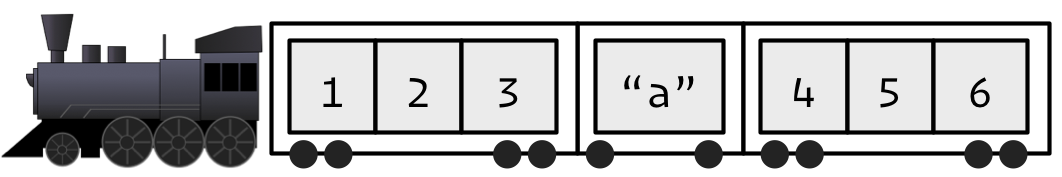
\includegraphics[width=3.54in]{images/subsetting/train} \end{center}

When extracting a single element, you have two options: you can create a
smaller train, or you can extract the contents of a carriage. This is
the difference between \texttt{{[}} and \texttt{{[}{[}}:

\begin{center}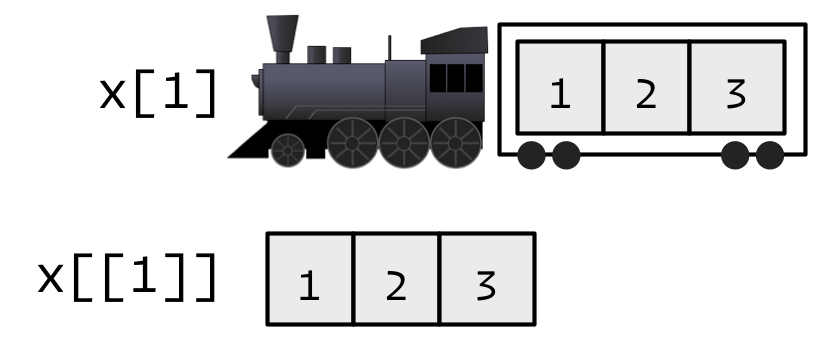
\includegraphics[width=2.75in]{images/subsetting/train-single} \end{center}

When extracting multiple elements (or zero!), you have to make a smaller
train:

\begin{center}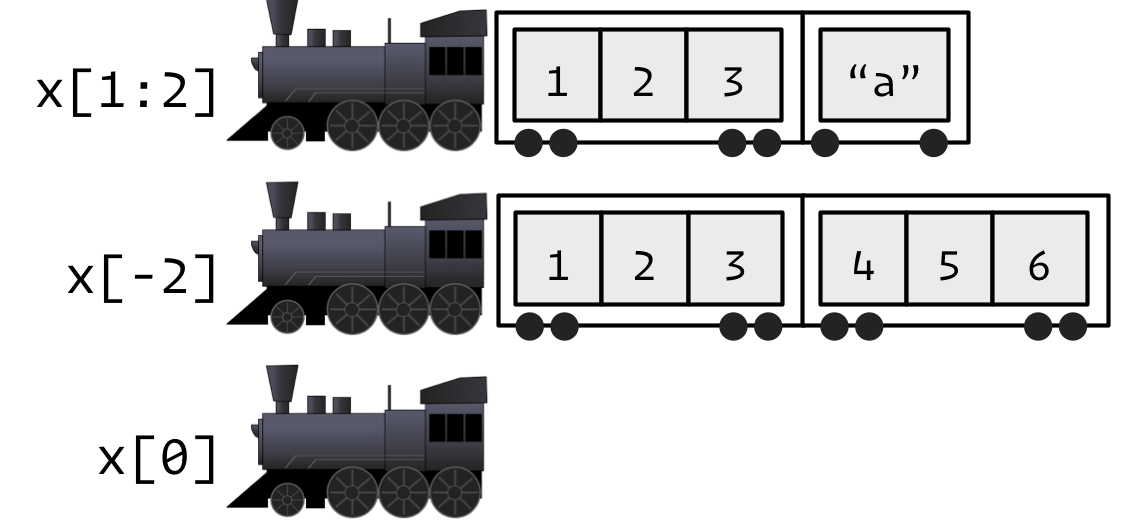
\includegraphics[width=3.74in]{images/subsetting/train-multiple} \end{center}

Because it can return only a single value, you must use \texttt{{[}{[}}
with either a single positive integer or a string. Because data frames
are lists of columns, you can use \texttt{{[}{[}} to extract a column
from data frames: \texttt{mtcars{[}{[}1{]}{]}},
\texttt{mtcars{[}{[}"cyl"{]}{]}}.

If you use a vector with \texttt{{[}{[}}, it will subset recursively:

\begin{Shaded}
\begin{Highlighting}[]
\NormalTok{(b <-}\StringTok{ }\KeywordTok{list}\NormalTok{(}\DataTypeTok{a =} \KeywordTok{list}\NormalTok{(}\DataTypeTok{b =} \KeywordTok{list}\NormalTok{(}\DataTypeTok{c =} \KeywordTok{list}\NormalTok{(}\DataTypeTok{d =} \DecValTok{1}\NormalTok{)))))}
\CommentTok{#> $a}
\CommentTok{#> $a$b}
\CommentTok{#> $a$b$c}
\CommentTok{#> $a$b$c$d}
\CommentTok{#> [1] 1}
\NormalTok{b[[}\KeywordTok{c}\NormalTok{(}\StringTok{"a"}\NormalTok{, }\StringTok{"b"}\NormalTok{, }\StringTok{"c"}\NormalTok{, }\StringTok{"d"}\NormalTok{)]]}
\CommentTok{#> [1] 1}

\CommentTok{# Equivalent to}
\NormalTok{b[[}\StringTok{"a"}\NormalTok{]][[}\StringTok{"b"}\NormalTok{]][[}\StringTok{"c"}\NormalTok{]][[}\StringTok{"d"}\NormalTok{]]}
\CommentTok{#> [1] 1}
\end{Highlighting}
\end{Shaded}

\texttt{{[}{[}} is crucial for working with lists, but I recommend using
it whenever you want your code to clearly express that it's working with
a single value. That frequently arises in for loops, i.e.~instead of
writing:

\begin{Shaded}
\begin{Highlighting}[]
\ControlFlowTok{for}\NormalTok{ (i }\ControlFlowTok{in} \DecValTok{2}\OperatorTok{:}\KeywordTok{length}\NormalTok{(x)) \{}
\NormalTok{  out[i] <-}\StringTok{ }\KeywordTok{fun}\NormalTok{(x[i], out[i }\OperatorTok{-}\StringTok{ }\DecValTok{1}\NormalTok{])}
\NormalTok{\}}
\end{Highlighting}
\end{Shaded}

It's better to write:

\begin{Shaded}
\begin{Highlighting}[]
\ControlFlowTok{for}\NormalTok{ (i }\ControlFlowTok{in} \DecValTok{2}\OperatorTok{:}\KeywordTok{length}\NormalTok{(x)) \{}
\NormalTok{  out[[i]] <-}\StringTok{ }\KeywordTok{fun}\NormalTok{(x[[i]], out[[i }\OperatorTok{-}\StringTok{ }\DecValTok{1}\NormalTok{]])}
\NormalTok{\}}
\end{Highlighting}
\end{Shaded}

\subsection{\texorpdfstring{\texttt{\$}}{\$}}\label{section}

\texttt{\$} is a shorthand operator: \texttt{x\$y} is roughly equivalent
to \texttt{x{[}{[}"y"{]}{]}}. It's often used to access variables in a
data frame, as in \texttt{mtcars\$cyl} or \texttt{diamonds\$carat}. One
common mistake with \texttt{\$} is to try and use it when you have the
name of a column stored in a variable:

\begin{Shaded}
\begin{Highlighting}[]
\NormalTok{var <-}\StringTok{ "cyl"}
\CommentTok{# Doesn't work - mtcars$var translated to mtcars[["var"]]}
\NormalTok{mtcars}\OperatorTok{$}\NormalTok{var}
\CommentTok{#> NULL}

\CommentTok{# Instead use [[}
\NormalTok{mtcars[[var]]}
\CommentTok{#>  [1] 6 6 4 6 8 6 8 4 4 6 6 8 8 8 8 8 8 4 4 4 4 8 8 8 8 4 4 4 8 6 8 4}
\end{Highlighting}
\end{Shaded}

There's one important difference between \texttt{\$} and
\texttt{{[}{[}}. \texttt{\$} does partial matching:

\begin{Shaded}
\begin{Highlighting}[]
\NormalTok{x <-}\StringTok{ }\KeywordTok{list}\NormalTok{(}\DataTypeTok{abc =} \DecValTok{1}\NormalTok{)}
\NormalTok{x}\OperatorTok{$}\NormalTok{a}
\CommentTok{#> [1] 1}
\NormalTok{x[[}\StringTok{"a"}\NormalTok{]]}
\CommentTok{#> NULL}
\end{Highlighting}
\end{Shaded}

It is usually a good idea to \textbf{NOT} use partial matching. It tends
to to lead to hard to track down bugs and makes your code much less
readable. With auto complete in RStudio it tends not to save any time or
keystrokes.

\subsection{Missing/out of bounds
indices}\label{missingout-of-bounds-indices}

TL;DR version use \texttt{purrr::pluck()}, which we will get to in
\emph{R for Data Science}

It's useful to understand what happens with \texttt{{[}} and
\texttt{{[}{[}} when you use an ``invalid'' index. The following tables
summarize what happen when you subset a logical vector, list, and
\texttt{NULL} with an out-of-bounds value (OOB), a missing value (i.e
\texttt{NA\_integer\_}), and a zero-length object (like \texttt{NULL} or
\texttt{logical()}) with \texttt{{[}} and \texttt{{[}{[}}. Each cell
shows the result of subsetting the data structure named in the row by
the type of index described in the column. I've only shown the results
for logical vectors, but other atomic vectors behave similarly,
returning elements of the same type.

\begin{longtable}[]{@{}llll@{}}
\toprule
\texttt{row{[}col{]}} & Zero-length & OOB & Missing\tabularnewline
\midrule
\endhead
\texttt{NULL} & \texttt{NULL} & \texttt{NULL} &
\texttt{NULL}\tabularnewline
Logical & \texttt{logical(0)} & \texttt{NA} & \texttt{NA}\tabularnewline
List & \texttt{list()} & \texttt{list(NULL)} &
\texttt{list(NULL)}\tabularnewline
\bottomrule
\end{longtable}

With \texttt{{[}}, it doesn't matter whether the OOB index is a position
or a name, but it does for \texttt{{[}{[}}:

\begin{longtable}[]{@{}lllll@{}}
\toprule
\texttt{row{[}{[}col{]}{]}} & Zero-length & OOB (int) & OOB (chr) &
Missing\tabularnewline
\midrule
\endhead
\texttt{NULL} & \texttt{NULL} & \texttt{NULL} & \texttt{NULL} &
\texttt{NULL}\tabularnewline
Atomic & Error & Error & Error & Error\tabularnewline
List & Error & Error & \texttt{NULL} & \texttt{NULL}\tabularnewline
\bottomrule
\end{longtable}

If the input vector is named, then the names of OOB, missing, or
\texttt{NULL} components will be \texttt{"\textless{}NA\textgreater{}"}.

\section{Subsetting and assignment}\label{subassignment}

All subsetting operators can be combined with assignment to modify
selected values of the input vector.

\begin{Shaded}
\begin{Highlighting}[]
\NormalTok{x <-}\StringTok{ }\DecValTok{1}\OperatorTok{:}\DecValTok{5}
\NormalTok{x[}\KeywordTok{c}\NormalTok{(}\DecValTok{1}\NormalTok{, }\DecValTok{2}\NormalTok{)] <-}\StringTok{ }\DecValTok{2}\OperatorTok{:}\DecValTok{3}
\NormalTok{x}
\CommentTok{#> [1] 2 3 3 4 5}

\CommentTok{# The length of the LHS needs to match the RHS}
\NormalTok{x[}\OperatorTok{-}\DecValTok{1}\NormalTok{] <-}\StringTok{ }\DecValTok{4}\OperatorTok{:}\DecValTok{1}
\NormalTok{x}
\CommentTok{#> [1] 2 4 3 2 1}

\CommentTok{# Duplicated indices go unchecked and may be problematic}
\NormalTok{x[}\KeywordTok{c}\NormalTok{(}\DecValTok{1}\NormalTok{, }\DecValTok{1}\NormalTok{)] <-}\StringTok{ }\DecValTok{2}\OperatorTok{:}\DecValTok{3}
\NormalTok{x}
\CommentTok{#> [1] 3 4 3 2 1}

\CommentTok{# You can't combine integer indices with NA}
\NormalTok{x[}\KeywordTok{c}\NormalTok{(}\DecValTok{1}\NormalTok{, }\OtherTok{NA}\NormalTok{)] <-}\StringTok{ }\KeywordTok{c}\NormalTok{(}\DecValTok{1}\NormalTok{, }\DecValTok{2}\NormalTok{)}
\CommentTok{#> Error in x[c(1, NA)] <- c(1, 2): NAs are not allowed in subscripted assignments}
\CommentTok{# But you can combine logical indices with NA}
\CommentTok{# (where they're treated as false).}
\NormalTok{x[}\KeywordTok{c}\NormalTok{(T, F, }\OtherTok{NA}\NormalTok{)] <-}\StringTok{ }\DecValTok{1}
\NormalTok{x}
\CommentTok{#> [1] 1 4 3 1 1}

\CommentTok{# This is mostly useful when conditionally modifying vectors}
\NormalTok{df <-}\StringTok{ }\KeywordTok{data.frame}\NormalTok{(}\DataTypeTok{a =} \KeywordTok{c}\NormalTok{(}\DecValTok{1}\NormalTok{, }\DecValTok{10}\NormalTok{, }\OtherTok{NA}\NormalTok{))}
\NormalTok{df}\OperatorTok{$}\NormalTok{a[df}\OperatorTok{$}\NormalTok{a }\OperatorTok{<}\StringTok{ }\DecValTok{5}\NormalTok{] <-}\StringTok{ }\DecValTok{0}
\NormalTok{df}\OperatorTok{$}\NormalTok{a}
\CommentTok{#> [1]  0 10 NA}
\end{Highlighting}
\end{Shaded}

Subsetting with nothing can be useful in conjunction with assignment
because it will preserve the original object class and structure.
Compare the following two expressions. In the first, \texttt{mtcars}
will remain as a data frame. In the second, \texttt{mtcars} will become
a list.

\begin{Shaded}
\begin{Highlighting}[]
\NormalTok{(mtcars[] <-}\StringTok{ }\KeywordTok{lapply}\NormalTok{(mtcars, as.integer))}
\NormalTok{(mtcars <-}\StringTok{ }\KeywordTok{lapply}\NormalTok{(mtcars, as.integer))}
\end{Highlighting}
\end{Shaded}

With lists, you can use \texttt{{[}{[}} + assignment + \texttt{NULL} to
remove components from a list. To add a literal \texttt{NULL} to a list,
use \texttt{{[}} and \texttt{list(NULL)}:

\begin{Shaded}
\begin{Highlighting}[]
\NormalTok{x <-}\StringTok{ }\KeywordTok{list}\NormalTok{(}\DataTypeTok{a =} \DecValTok{1}\NormalTok{, }\DataTypeTok{b =} \DecValTok{2}\NormalTok{)}
\NormalTok{x[[}\StringTok{"b"}\NormalTok{]] <-}\StringTok{ }\OtherTok{NULL}
\KeywordTok{str}\NormalTok{(x)}
\CommentTok{#> List of 1}
\CommentTok{#>  $ a: num 1}

\NormalTok{y <-}\StringTok{ }\KeywordTok{list}\NormalTok{(}\DataTypeTok{a =} \DecValTok{1}\NormalTok{)}
\NormalTok{y[}\StringTok{"b"}\NormalTok{] <-}\StringTok{ }\KeywordTok{list}\NormalTok{(}\OtherTok{NULL}\NormalTok{)}
\KeywordTok{str}\NormalTok{(y)}
\CommentTok{#> List of 2}
\CommentTok{#>  $ a: num 1}
\CommentTok{#>  $ b: NULL}
\end{Highlighting}
\end{Shaded}

\section{Applications}\label{applications}

The basic principles described above give rise to a wide variety of
useful applications. Some of the most important are described below.
Many of these basic techniques are wrapped up into more concise
functions (e.g., \texttt{subset()}, \texttt{merge()},
\texttt{dplyr::arrange()}), but it is useful to understand how they are
implemented with basic subsetting. This will allow you to adapt to new
situations that are not dealt with by existing functions.

\subsection{Lookup tables (character
subsetting)}\label{lookup-tables-character-subsetting}

Character matching provides a powerful way to make look-up tables. Say
you want to convert abbreviations:

\begin{Shaded}
\begin{Highlighting}[]
\NormalTok{x <-}\StringTok{ }\KeywordTok{c}\NormalTok{(}\StringTok{"m"}\NormalTok{, }\StringTok{"f"}\NormalTok{, }\StringTok{"u"}\NormalTok{, }\StringTok{"f"}\NormalTok{, }\StringTok{"f"}\NormalTok{, }\StringTok{"m"}\NormalTok{, }\StringTok{"m"}\NormalTok{)}
\NormalTok{lookup <-}\StringTok{ }\KeywordTok{c}\NormalTok{(}\DataTypeTok{m =} \StringTok{"Male"}\NormalTok{, }\DataTypeTok{f =} \StringTok{"Female"}\NormalTok{, }\DataTypeTok{u =} \OtherTok{NA}\NormalTok{)}
\NormalTok{lookup[x]}
\CommentTok{#>        m        f        u        f        f        m        m }
\CommentTok{#>   "Male" "Female"       NA "Female" "Female"   "Male"   "Male"}

\KeywordTok{unname}\NormalTok{(lookup[x])}
\CommentTok{#> [1] "Male"   "Female" NA       "Female" "Female" "Male"   "Male"}
\end{Highlighting}
\end{Shaded}

If you don't want names in the result, use \texttt{unname()} to remove
them.

\subsection{Ordering (integer
subsetting)}\label{ordering-integer-subsetting}

\texttt{order()} takes a vector as input and returns an integer vector
describing how the subsetted vector should be ordered:

\begin{Shaded}
\begin{Highlighting}[]
\NormalTok{x <-}\StringTok{ }\KeywordTok{c}\NormalTok{(}\StringTok{"b"}\NormalTok{, }\StringTok{"c"}\NormalTok{, }\StringTok{"a"}\NormalTok{)}
\KeywordTok{order}\NormalTok{(x)}
\CommentTok{#> [1] 3 1 2}
\NormalTok{x[}\KeywordTok{order}\NormalTok{(x)]}
\CommentTok{#> [1] "a" "b" "c"}
\end{Highlighting}
\end{Shaded}

To break ties, you can supply additional variables to \texttt{order()},
and you can change from ascending to descending order using
\texttt{decreasing\ =\ TRUE}. By default, any missing values will be put
at the end of the vector; however, you can remove them with
\texttt{na.last\ =\ NA} or put at the front with
\texttt{na.last\ =\ FALSE}.

For two or more dimensions, \texttt{order()} and integer subsetting
makes it easy to order either the rows or columns of an object:

\begin{Shaded}
\begin{Highlighting}[]
\NormalTok{(df <-}\StringTok{ }\KeywordTok{data.frame}\NormalTok{(}\DataTypeTok{x =} \KeywordTok{rep}\NormalTok{(}\DecValTok{1}\OperatorTok{:}\DecValTok{3}\NormalTok{, }\DataTypeTok{each =} \DecValTok{2}\NormalTok{), }\DataTypeTok{y =} \DecValTok{6}\OperatorTok{:}\DecValTok{1}\NormalTok{, }\DataTypeTok{z =}\NormalTok{ letters[}\DecValTok{1}\OperatorTok{:}\DecValTok{6}\NormalTok{]))}
\CommentTok{#>   x y z}
\CommentTok{#> 1 1 6 a}
\CommentTok{#> 2 1 5 b}
\CommentTok{#> 3 2 4 c}
\CommentTok{#> 4 2 3 d}
\CommentTok{#> 5 3 2 e}
\CommentTok{#> 6 3 1 f}
\CommentTok{# Randomly reorder df}
\NormalTok{df2 <-}\StringTok{ }\NormalTok{df[}\KeywordTok{sample}\NormalTok{(}\KeywordTok{nrow}\NormalTok{(df)), }\DecValTok{3}\OperatorTok{:}\DecValTok{1}\NormalTok{]}
\NormalTok{df2}
\CommentTok{#>   z y x}
\CommentTok{#> 3 c 4 2}
\CommentTok{#> 2 b 5 1}
\CommentTok{#> 5 e 2 3}
\CommentTok{#> 6 f 1 3}
\CommentTok{#> 4 d 3 2}
\CommentTok{#> 1 a 6 1}

\NormalTok{df2[}\KeywordTok{order}\NormalTok{(df2}\OperatorTok{$}\NormalTok{x), ]}
\CommentTok{#>   z y x}
\CommentTok{#> 2 b 5 1}
\CommentTok{#> 1 a 6 1}
\CommentTok{#> 3 c 4 2}
\CommentTok{#> 4 d 3 2}
\CommentTok{#> 5 e 2 3}
\CommentTok{#> 6 f 1 3}
\NormalTok{df2[, }\KeywordTok{order}\NormalTok{(}\KeywordTok{names}\NormalTok{(df2))]}
\CommentTok{#>   x y z}
\CommentTok{#> 3 2 4 c}
\CommentTok{#> 2 1 5 b}
\CommentTok{#> 5 3 2 e}
\CommentTok{#> 6 3 1 f}
\CommentTok{#> 4 2 3 d}
\CommentTok{#> 1 1 6 a}
\end{Highlighting}
\end{Shaded}

You can sort vectors directly with \texttt{sort()}, or use
\texttt{dplyr::arrange()} or similar to sort a data frame.

\subsection{Selecting rows based on a condition (logical
subsetting)}\label{selecting-rows-based-on-a-condition-logical-subsetting}

Because it allows you to easily combine conditions from multiple
columns, logical subsetting is probably the most commonly used technique
for extracting rows out of a data frame.

\begin{Shaded}
\begin{Highlighting}[]
\NormalTok{mtcars[mtcars}\OperatorTok{$}\NormalTok{gear }\OperatorTok{==}\StringTok{ }\DecValTok{5}\NormalTok{, ]}
\CommentTok{#>                 mpg cyl  disp  hp drat   wt qsec vs am gear carb}
\CommentTok{#> Porsche 914-2  26.0   4 120.3  91 4.43 2.14 16.7  0  1    5    2}
\CommentTok{#> Lotus Europa   30.4   4  95.1 113 3.77 1.51 16.9  1  1    5    2}
\CommentTok{#> Ford Pantera L 15.8   8 351.0 264 4.22 3.17 14.5  0  1    5    4}
\CommentTok{#> Ferrari Dino   19.7   6 145.0 175 3.62 2.77 15.5  0  1    5    6}
\CommentTok{#> Maserati Bora  15.0   8 301.0 335 3.54 3.57 14.6  0  1    5    8}

\NormalTok{mtcars[mtcars}\OperatorTok{$}\NormalTok{gear }\OperatorTok{==}\StringTok{ }\DecValTok{5} \OperatorTok{&}\StringTok{ }\NormalTok{mtcars}\OperatorTok{$}\NormalTok{cyl }\OperatorTok{==}\StringTok{ }\DecValTok{4}\NormalTok{, ]}
\CommentTok{#>                mpg cyl  disp  hp drat   wt qsec vs am gear carb}
\CommentTok{#> Porsche 914-2 26.0   4 120.3  91 4.43 2.14 16.7  0  1    5    2}
\CommentTok{#> Lotus Europa  30.4   4  95.1 113 3.77 1.51 16.9  1  1    5    2}
\end{Highlighting}
\end{Shaded}

Remember to use the vector boolean operators \texttt{\&} and
\texttt{\textbar{}}, not the short-circuiting scalar operators
\texttt{\&\&} and \texttt{\textbar{}\textbar{}} which are more useful
inside if statements. Don't forget
\href{https://en.wikipedia.org/wiki/De_Morgan\%27s_laws}{De Morgan's
laws}, which can be useful to simplify negations:

\begin{itemize}
\tightlist
\item
  \texttt{!(X\ \&\ Y)} is the same as \texttt{!X\ \textbar{}\ !Y}
\item
  \texttt{!(X\ \textbar{}\ Y)} is the same as \texttt{!X\ \&\ !Y}
\end{itemize}

For example, \texttt{!(X\ \&\ !(Y\ \textbar{}\ Z))} simplifies to
\texttt{!X\ \textbar{}\ !!(Y\textbar{}Z)}, and then to
\texttt{!X\ \textbar{}\ Y\ \textbar{}\ Z}.

\texttt{subset()} is a specialized shorthand function for subsetting
data frames, and saves some typing because you don't need to repeat the
name of the data frame..

\begin{Shaded}
\begin{Highlighting}[]
\KeywordTok{subset}\NormalTok{(mtcars, gear }\OperatorTok{==}\StringTok{ }\DecValTok{5}\NormalTok{)}
\CommentTok{#>                 mpg cyl  disp  hp drat   wt qsec vs am gear carb}
\CommentTok{#> Porsche 914-2  26.0   4 120.3  91 4.43 2.14 16.7  0  1    5    2}
\CommentTok{#> Lotus Europa   30.4   4  95.1 113 3.77 1.51 16.9  1  1    5    2}
\CommentTok{#> Ford Pantera L 15.8   8 351.0 264 4.22 3.17 14.5  0  1    5    4}
\CommentTok{#> Ferrari Dino   19.7   6 145.0 175 3.62 2.77 15.5  0  1    5    6}
\CommentTok{#> Maserati Bora  15.0   8 301.0 335 3.54 3.57 14.6  0  1    5    8}

\KeywordTok{subset}\NormalTok{(mtcars, gear }\OperatorTok{==}\StringTok{ }\DecValTok{5} \OperatorTok{&}\StringTok{ }\NormalTok{cyl }\OperatorTok{==}\StringTok{ }\DecValTok{4}\NormalTok{)}
\CommentTok{#>                mpg cyl  disp  hp drat   wt qsec vs am gear carb}
\CommentTok{#> Porsche 914-2 26.0   4 120.3  91 4.43 2.14 16.7  0  1    5    2}
\CommentTok{#> Lotus Europa  30.4   4  95.1 113 3.77 1.51 16.9  1  1    5    2}
\end{Highlighting}
\end{Shaded}

\subsection{Boolean algebra vs.~sets (logical \& integer
subsetting)}\label{boolean-algebra-vs.sets-logical-integer-subsetting}

It's useful to be aware of the natural equivalence between set
operations (integer subsetting) and boolean algebra (logical
subsetting). Using set operations is more effective when:

\begin{itemize}
\item
  You want to find the first (or last) \texttt{TRUE}.
\item
  You have very few \texttt{TRUE}s and very many \texttt{FALSE}s; a set
  representation may be faster and require less storage.
\end{itemize}

\texttt{which()} allows you to convert a boolean representation to an
integer representation.

Let's create two logical vectors and their integer equivalents and then
explore the relationship between boolean and set operations.

\begin{Shaded}
\begin{Highlighting}[]
\NormalTok{(x1 <-}\StringTok{ }\DecValTok{1}\OperatorTok{:}\DecValTok{10} \OperatorTok\StringTok{ }\DecValTok{2} \OperatorTok{==}\StringTok{ }\DecValTok{0}\NormalTok{)}
\CommentTok{#>  [1] FALSE  TRUE FALSE  TRUE FALSE  TRUE FALSE  TRUE FALSE  TRUE}
\NormalTok{(x2 <-}\StringTok{ }\KeywordTok{which}\NormalTok{(x1))}
\CommentTok{#> [1]  2  4  6  8 10}
\NormalTok{(y1 <-}\StringTok{ }\DecValTok{1}\OperatorTok{:}\DecValTok{10} \OperatorTok\StringTok{ }\DecValTok{5} \OperatorTok{==}\StringTok{ }\DecValTok{0}\NormalTok{)}
\CommentTok{#>  [1] FALSE FALSE FALSE FALSE  TRUE FALSE FALSE FALSE FALSE  TRUE}
\NormalTok{(y2 <-}\StringTok{ }\KeywordTok{which}\NormalTok{(y1))}
\CommentTok{#> [1]  5 10}

\CommentTok{# X & Y <-> intersect(x, y)}
\NormalTok{x1 }\OperatorTok{&}\StringTok{ }\NormalTok{y1}
\CommentTok{#>  [1] FALSE FALSE FALSE FALSE FALSE FALSE FALSE FALSE FALSE  TRUE}
\KeywordTok{intersect}\NormalTok{(x2, y2)}
\CommentTok{#> [1] 10}

\CommentTok{# X | Y <-> union(x, y)}
\NormalTok{x1 }\OperatorTok{|}\StringTok{ }\NormalTok{y1}
\CommentTok{#>  [1] FALSE  TRUE FALSE  TRUE  TRUE  TRUE FALSE  TRUE FALSE  TRUE}
\KeywordTok{union}\NormalTok{(x2, y2)}
\CommentTok{#> [1]  2  4  6  8 10  5}

\CommentTok{# X & !Y <-> setdiff(x, y)}
\NormalTok{x1 }\OperatorTok{&}\StringTok{ }\OperatorTok{!}\NormalTok{y1}
\CommentTok{#>  [1] FALSE  TRUE FALSE  TRUE FALSE  TRUE FALSE  TRUE FALSE FALSE}
\KeywordTok{setdiff}\NormalTok{(x2, y2)}
\CommentTok{#> [1] 2 4 6 8}

\CommentTok{# xor(X, Y) <-> setdiff(union(x, y), intersect(x, y))}
\KeywordTok{xor}\NormalTok{(x1, y1)}
\CommentTok{#>  [1] FALSE  TRUE FALSE  TRUE  TRUE  TRUE FALSE  TRUE FALSE FALSE}
\KeywordTok{setdiff}\NormalTok{(}\KeywordTok{union}\NormalTok{(x2, y2), }\KeywordTok{intersect}\NormalTok{(x2, y2))}
\CommentTok{#> [1] 2 4 6 8 5}
\end{Highlighting}
\end{Shaded}

When first learning subsetting, a common mistake is to use
\texttt{x{[}which(y){]}} instead of \texttt{x{[}y{]}}. Here the
\texttt{which()} achieves nothing: it switches from logical to integer
subsetting but the result will be exactly the same. In more general
cases, there are two important differences. First, when the logical
vector contains NA, logical subsetting replaces these values by NA while
\texttt{which()} drops these values. Second, \texttt{x{[}-which(y){]}}
is \textbf{not} equivalent to \texttt{x{[}!y{]}}: if \texttt{y} is all
FALSE, \texttt{which(y)} will be \texttt{integer(0)} and
\texttt{-integer(0)} is still \texttt{integer(0)}, so you'll get no
values, instead of all values. In general, avoid switching from logical
to integer subsetting unless you want, for example, the first or last
\texttt{TRUE} value.

\subsection{Removing columns from data frames (character
subsetting)}\label{removing-columns-from-data-frames-character-subsetting}

There are two ways to remove columns from a data frame. You can set
individual columns to \texttt{NULL}:

\begin{Shaded}
\begin{Highlighting}[]
\NormalTok{df <-}\StringTok{ }\KeywordTok{data.frame}\NormalTok{(}\DataTypeTok{x =} \DecValTok{1}\OperatorTok{:}\DecValTok{3}\NormalTok{, }\DataTypeTok{y =} \DecValTok{3}\OperatorTok{:}\DecValTok{1}\NormalTok{, }\DataTypeTok{z =}\NormalTok{ letters[}\DecValTok{1}\OperatorTok{:}\DecValTok{3}\NormalTok{])}
\NormalTok{df}\OperatorTok{$}\NormalTok{z <-}\StringTok{ }\OtherTok{NULL}
\end{Highlighting}
\end{Shaded}

Or you can subset to return only the columns you want:

\begin{Shaded}
\begin{Highlighting}[]
\NormalTok{df <-}\StringTok{ }\KeywordTok{data.frame}\NormalTok{(}\DataTypeTok{x =} \DecValTok{1}\OperatorTok{:}\DecValTok{3}\NormalTok{, }\DataTypeTok{y =} \DecValTok{3}\OperatorTok{:}\DecValTok{1}\NormalTok{, }\DataTypeTok{z =}\NormalTok{ letters[}\DecValTok{1}\OperatorTok{:}\DecValTok{3}\NormalTok{])}
\NormalTok{df[}\KeywordTok{c}\NormalTok{(}\StringTok{"x"}\NormalTok{, }\StringTok{"y"}\NormalTok{)]}
\CommentTok{#>   x y}
\CommentTok{#> 1 1 3}
\CommentTok{#> 2 2 2}
\CommentTok{#> 3 3 1}
\end{Highlighting}
\end{Shaded}

If you know the columns you don't want, use set operations to work out
which columns to keep:

\begin{Shaded}
\begin{Highlighting}[]
\NormalTok{df[}\KeywordTok{setdiff}\NormalTok{(}\KeywordTok{names}\NormalTok{(df), }\StringTok{"z"}\NormalTok{)]}
\CommentTok{#>   x y}
\CommentTok{#> 1 1 3}
\CommentTok{#> 2 2 2}
\CommentTok{#> 3 3 1}
\end{Highlighting}
\end{Shaded}

\subsection{Matching and merging by hand (integer
subsetting)}\label{matching-and-merging-by-hand-integer-subsetting}

You may have a more complicated look-up table which has multiple columns
of information. Suppose we have a vector of integer grades, and a table
that describes their properties:

\begin{Shaded}
\begin{Highlighting}[]
\NormalTok{grades <-}\StringTok{ }\KeywordTok{c}\NormalTok{(}\DecValTok{1}\NormalTok{, }\DecValTok{2}\NormalTok{, }\DecValTok{2}\NormalTok{, }\DecValTok{3}\NormalTok{, }\DecValTok{1}\NormalTok{)}

\NormalTok{info <-}\StringTok{ }\KeywordTok{data.frame}\NormalTok{(}
  \DataTypeTok{grade =} \DecValTok{3}\OperatorTok{:}\DecValTok{1}\NormalTok{,}
  \DataTypeTok{desc =} \KeywordTok{c}\NormalTok{(}\StringTok{"Excellent"}\NormalTok{, }\StringTok{"Good"}\NormalTok{, }\StringTok{"Poor"}\NormalTok{),}
  \DataTypeTok{fail =} \KeywordTok{c}\NormalTok{(F, F, T)}
\NormalTok{)}
\end{Highlighting}
\end{Shaded}

We want to duplicate the info table so that we have a row for each value
in \texttt{grades}. An elegant way to do this is by combining
\texttt{match()} and integer subsetting:

\begin{Shaded}
\begin{Highlighting}[]
\NormalTok{id <-}\StringTok{ }\KeywordTok{match}\NormalTok{(grades, info}\OperatorTok{$}\NormalTok{grade)}
\NormalTok{info[id, ]}
\CommentTok{#>     grade      desc  fail}
\CommentTok{#> 3       1      Poor  TRUE}
\CommentTok{#> 2       2      Good FALSE}
\CommentTok{#> 2.1     2      Good FALSE}
\CommentTok{#> 1       3 Excellent FALSE}
\CommentTok{#> 3.1     1      Poor  TRUE}
\end{Highlighting}
\end{Shaded}

If you have multiple columns to match on, you'll need to first collapse
them to a single column (with e.g. \texttt{interaction()}), but
typically you are better off switching to a function design specifically
for joining multiple tables like \texttt{merge()}, or
\texttt{dplyr::left\_join()}.

\subsection{Random samples/bootstrap (integer
subsetting)}\label{random-samplesbootstrap-integer-subsetting}

You can use integer indices to perform random sampling or bootstrapping
of a vector or data frame. \texttt{sample()} generates a vector of
indices, then subsetting accesses the values:

\begin{Shaded}
\begin{Highlighting}[]
\NormalTok{(df <-}\StringTok{ }\KeywordTok{data.frame}\NormalTok{(}\DataTypeTok{x =} \KeywordTok{rep}\NormalTok{(}\DecValTok{1}\OperatorTok{:}\DecValTok{3}\NormalTok{, }\DataTypeTok{each =} \DecValTok{2}\NormalTok{), }\DataTypeTok{y =} \DecValTok{6}\OperatorTok{:}\DecValTok{1}\NormalTok{, }\DataTypeTok{z =}\NormalTok{ letters[}\DecValTok{1}\OperatorTok{:}\DecValTok{6}\NormalTok{]))}
\CommentTok{#>   x y z}
\CommentTok{#> 1 1 6 a}
\CommentTok{#> 2 1 5 b}
\CommentTok{#> 3 2 4 c}
\CommentTok{#> 4 2 3 d}
\CommentTok{#> 5 3 2 e}
\CommentTok{#> 6 3 1 f}

\CommentTok{# Randomly reorder}
\NormalTok{df[}\KeywordTok{sample}\NormalTok{(}\KeywordTok{nrow}\NormalTok{(df)), ]}
\CommentTok{#>   x y z}
\CommentTok{#> 5 3 2 e}
\CommentTok{#> 4 2 3 d}
\CommentTok{#> 1 1 6 a}
\CommentTok{#> 3 2 4 c}
\CommentTok{#> 6 3 1 f}
\CommentTok{#> 2 1 5 b}

\CommentTok{# Select 3 random rows}
\NormalTok{df[}\KeywordTok{sample}\NormalTok{(}\KeywordTok{nrow}\NormalTok{(df), }\DecValTok{3}\NormalTok{), ]}
\CommentTok{#>   x y z}
\CommentTok{#> 6 3 1 f}
\CommentTok{#> 5 3 2 e}
\CommentTok{#> 3 2 4 c}

\CommentTok{# Select 6 bootstrap replicates}
\NormalTok{df[}\KeywordTok{sample}\NormalTok{(}\KeywordTok{nrow}\NormalTok{(df), }\DecValTok{6}\NormalTok{, }\DataTypeTok{rep =} \OtherTok{TRUE}\NormalTok{), ]}
\CommentTok{#>     x y z}
\CommentTok{#> 2   1 5 b}
\CommentTok{#> 6   3 1 f}
\CommentTok{#> 3   2 4 c}
\CommentTok{#> 3.1 2 4 c}
\CommentTok{#> 6.1 3 1 f}
\CommentTok{#> 1   1 6 a}
\end{Highlighting}
\end{Shaded}

The arguments of \texttt{sample()} control the number of samples to
extract, and whether sampling is performed with or without replacement.

\subsection{Expanding aggregated counts (integer
subsetting)}\label{expanding-aggregated-counts-integer-subsetting}

Sometimes you get a data frame where identical rows have been collapsed
into one and a count column has been added. \texttt{rep()} and integer
subsetting make it easy to uncollapse the data by subsetting with a
repeated row index:

\begin{Shaded}
\begin{Highlighting}[]
\NormalTok{df <-}\StringTok{ }\KeywordTok{data.frame}\NormalTok{(}\DataTypeTok{x =} \KeywordTok{c}\NormalTok{(}\DecValTok{2}\NormalTok{, }\DecValTok{4}\NormalTok{, }\DecValTok{1}\NormalTok{), }\DataTypeTok{y =} \KeywordTok{c}\NormalTok{(}\DecValTok{9}\NormalTok{, }\DecValTok{11}\NormalTok{, }\DecValTok{6}\NormalTok{), }\DataTypeTok{n =} \KeywordTok{c}\NormalTok{(}\DecValTok{3}\NormalTok{, }\DecValTok{5}\NormalTok{, }\DecValTok{1}\NormalTok{))}
\NormalTok{df}
\CommentTok{#>   x  y n}
\CommentTok{#> 1 2  9 3}
\CommentTok{#> 2 4 11 5}
\CommentTok{#> 3 1  6 1}
\KeywordTok{rep}\NormalTok{(}\DecValTok{1}\OperatorTok{:}\KeywordTok{nrow}\NormalTok{(df), df}\OperatorTok{$}\NormalTok{n)}
\CommentTok{#> [1] 1 1 1 2 2 2 2 2 3}

\NormalTok{df[}\KeywordTok{rep}\NormalTok{(}\DecValTok{1}\OperatorTok{:}\KeywordTok{nrow}\NormalTok{(df), df}\OperatorTok{$}\NormalTok{n), ]}
\CommentTok{#>     x  y n}
\CommentTok{#> 1   2  9 3}
\CommentTok{#> 1.1 2  9 3}
\CommentTok{#> 1.2 2  9 3}
\CommentTok{#> 2   4 11 5}
\CommentTok{#> 2.1 4 11 5}
\CommentTok{#> 2.2 4 11 5}
\CommentTok{#> 2.3 4 11 5}
\CommentTok{#> 2.4 4 11 5}
\CommentTok{#> 3   1  6 1}
\end{Highlighting}
\end{Shaded}

\section{Exercises}\label{exercises-2}

\begin{enumerate}
\def\labelenumi{\arabic{enumi}.}
\tightlist
\item
  \texttt{which()} allows you to convert a boolean representation to an
  integer representation. There's no reverse operation in base R. Create
  an \texttt{unwhich} function. \texttt{unwhich(which(x),\ length(x))}
  should return your original vector.
\end{enumerate}

\begin{Shaded}
\begin{Highlighting}[]
\NormalTok{x <-}\StringTok{ }\KeywordTok{sample}\NormalTok{(}\DecValTok{10}\NormalTok{) }\OperatorTok{<}\StringTok{ }\DecValTok{4}
\KeywordTok{which}\NormalTok{(x)}

\NormalTok{unwhich <-}\StringTok{ }\ControlFlowTok{function}\NormalTok{(x, n) \{}
  \CommentTok{# your code here}
\NormalTok{\}}
\KeywordTok{unwhich}\NormalTok{(}\KeywordTok{which}\NormalTok{(x), }\DecValTok{10}\NormalTok{)}
\end{Highlighting}
\end{Shaded}

\bibliography{book.bib,packages.bib}


\end{document}
